% ============================================================================
%  SETU: Multilingual Preference Distillation for Offline Indian Language
%        SLM Translators
%  Project Phase-II Report
%  Dept. of Artificial Intelligence & Machine Learning
%  Bangalore Institute of Technology, Bengaluru - 560004
%
%  Build:  tectonic -X compile main.tex      (or:  xelatex main.tex  x3 )
% ============================================================================
\documentclass[12pt, a4paper, oneside]{report}

% ============================================================================
%  SETU -- Project Phase-II Report : preamble
%  Formatting follows R.1.Guidelines.docx:
%    A4, 1.5 spacing, Times New Roman
%    Margins  : Left 1.25in, Right 1in, Top/Bottom 0.75in
%    Chapter  : number left justified 16pt ; title CAPS centered 18pt bold
%    Section  : 16pt bold, left justified ; Subsection : 14pt bold, left
%    Body     : 12pt
%    Header   : project title (right), suppressed on chapter-opening pages
%    Footer   : Department (left) | 2025-2026 (centre) | page no. (right)
% ============================================================================

% ---------- page geometry --------------------------------------------------
\usepackage[a4paper,
            left=1.25in, right=1.0in, top=0.75in, bottom=0.75in,
            includehead, includefoot, headsep=10pt, footskip=22pt]{geometry}

% ---------- fonts ----------------------------------------------------------
\usepackage{fontspec}

% Times New Roman clone shipped with TeX (metrically compatible).
\setmainfont{texgyretermes}[
  Extension      = .otf,
  UprightFont    = *-regular,
  BoldFont       = *-bold,
  ItalicFont     = *-italic,
  BoldItalicFont = *-bolditalic]
\setsansfont{texgyreheros}[
  Extension      = .otf,
  UprightFont    = *-regular,
  BoldFont       = *-bold,
  ItalicFont     = *-italic,
  BoldItalicFont = *-bolditalic]
\setmonofont{texgyrecursor}[
  Extension      = .otf,
  UprightFont    = *-regular,
  BoldFont       = *-bold,
  ItalicFont     = *-italic,
  BoldItalicFont = *-bolditalic,
  Scale          = 0.88]

% ---------- Indic script fonts (for the qualitative translation samples) ----
% Serif variants: they match the Times-like body text, and unlike the Sans
% Gujarati/Bengali faces they carry the ASCII punctuation the samples contain.
\newfontfamily\devafont{Noto Serif Devanagari}[Script=Devanagari, Scale=0.96]
\newfontfamily\bengfont{Noto Serif Bengali}[Script=Bengali, Scale=0.96]
\newfontfamily\gujrfont{Noto Serif Gujarati}[Script=Gujarati, Scale=0.96]
\newfontfamily\guruonfont{Noto Serif Gurmukhi}[Script=Gurmukhi, Scale=0.96]
\newfontfamily\oryafont{Noto Serif Oriya}[Script=Oriya, Scale=0.96]
\newfontfamily\tamlfont{Noto Serif Tamil}[Script=Tamil, Scale=0.96]
\newfontfamily\telufont{Noto Serif Telugu}[Script=Telugu, Scale=0.96]
\newfontfamily\kndafont{Noto Serif Kannada}[Script=Kannada, Scale=0.96]
\newfontfamily\mlymfont{Noto Serif Malayalam}[Script=Malayalam, Scale=0.96]

\newcommand{\dev}[1]{{\devafont #1}}      % Hindi, Marathi
\newcommand{\ben}[1]{{\bengfont #1}}      % Bengali, Assamese
\newcommand{\guj}[1]{{\gujrfont #1}}
\newcommand{\gur}[1]{{\guruonfont #1}}    % Punjabi
\newcommand{\ory}[1]{{\oryafont #1}}
\newcommand{\tam}[1]{{\tamlfont #1}}
\newcommand{\tel}[1]{{\telufont #1}}
\newcommand{\kan}[1]{{\kndafont #1}}
\newcommand{\mal}[1]{{\mlymfont #1}}

% ---------- spacing --------------------------------------------------------
\usepackage{setspace}
\onehalfspacing
\setlength{\parindent}{0.5in}          % "1 tab space at the beginning of each para"
\setlength{\parskip}{0.35em}
\usepackage{microtype}
% Allow hyphenation inside \texttt{...}: long identifiers, paths and flags would
% otherwise run into the margin.
\usepackage[htt]{hyphenat}
\setlength{\emergencystretch}{3em}

% ---------- tables, figures, graphics --------------------------------------
\usepackage{graphicx}
\usepackage{booktabs}
\usepackage{longtable}
\usepackage{tabularx}
\usepackage{array}
\usepackage{multirow}
\usepackage{makecell}
\usepackage{colortbl}
\usepackage[table,dvipsnames]{xcolor}
\usepackage{float}
\usepackage[font=normalsize,labelfont=bf,skip=6pt]{caption}
\captionsetup[table]{position=top}
\captionsetup[figure]{position=bottom}
\renewcommand{\arraystretch}{1.25}
% ragged2e gives \justifying, which justifies a p-column the way body text is
% justified (with hyphenation) rather than the ragged-right \raggedright.
\usepackage{ragged2e}

% Paragraph column types:
%   J{w}  justified   -- prose cells wide enough to justify cleanly (>= 4 cm)
%   L{w}  ragged right-- narrow prose cells, where justifying opens ugly gaps
%   C{w}  centred     -- short labels
%   R{w}  flush right -- numeric
\newcolumntype{J}[1]{>{\justifying\arraybackslash}p{#1}}
\newcolumntype{L}[1]{>{\raggedright\arraybackslash}p{#1}}
\newcolumntype{C}[1]{>{\centering\arraybackslash}p{#1}}
\newcolumntype{R}[1]{>{\raggedleft\arraybackslash}p{#1}}
\newcolumntype{Y}{>{\raggedright\arraybackslash}X}

\definecolor{headblue}{HTML}{DCE6F1}
\definecolor{rowgrey}{HTML}{F4F4F4}
\definecolor{inkgrey}{HTML}{555555}
\definecolor{passgreen}{HTML}{1B7A3D}
\definecolor{warnamber}{HTML}{A9600A}
\newcommand{\pass}{\textcolor{passgreen}{\textbf{Pass}}}
\newcommand{\near}{\textcolor{warnamber}{\textbf{Near}}}
\newcommand{\yes}{\textcolor{passgreen}{\textbf{Yes}}}

% ---------- lists ----------------------------------------------------------
\usepackage{enumitem}
\setlist[itemize]{leftmargin=0.55in, topsep=3pt, itemsep=2pt, parsep=0pt}
\setlist[enumerate]{leftmargin=0.55in, topsep=3pt, itemsep=2pt, parsep=0pt}
\setlist[description]{leftmargin=0.55in, topsep=3pt, itemsep=2pt}

% ---------- headings -------------------------------------------------------
\usepackage{titlesec}

\titleformat{\chapter}[display]
  {\normalfont\bfseries}
  {\fontsize{16}{20}\selectfont\raggedright CHAPTER \thechapter}
  {6pt}
  {\fontsize{18}{24}\selectfont\centering\MakeUppercase}
\titlespacing*{\chapter}{0pt}{0pt}{22pt}

\titleformat{\section}
  {\normalfont\fontsize{16}{19}\selectfont\bfseries\raggedright}{\thesection}{0.6em}{}
\titlespacing*{\section}{0pt}{16pt}{8pt}

\titleformat{\subsection}
  {\normalfont\fontsize{14}{17}\selectfont\bfseries\raggedright}{\thesubsection}{0.6em}{}
\titlespacing*{\subsection}{0pt}{12pt}{6pt}

\titleformat{\subsubsection}
  {\normalfont\fontsize{12}{15}\selectfont\bfseries\raggedright}{\thesubsubsection}{0.6em}{}
\titlespacing*{\subsubsection}{0pt}{10pt}{4pt}

\setcounter{secnumdepth}{3}
% Table of contents stops at section level (1.1, 1.2, 1.3). Subsections such as
% 1.3.1 stay numbered and visible in the chapter text but are kept out of the
% TOC to keep it short; secnumdepth above is deliberately left at 3.
\setcounter{tocdepth}{1}

% ---------- header / footer ------------------------------------------------
\usepackage{fancyhdr}
\usepackage{lastpage}

\newcommand{\projecttitle}{SETU: Multilingual Preference Distillation for Offline Indian Language SLM Translators}
\newcommand{\shorttitle}{SETU: Offline Indian Language SLM Translators}
\newcommand{\deptname}{Dept. of AI \& ML, BIT}
\newcommand{\acadyear}{2025-2026}

\fancypagestyle{setumain}{%
  \fancyhf{}
  \renewcommand{\headrulewidth}{0.4pt}
  \renewcommand{\footrulewidth}{0.4pt}
  \fancyhead[R]{\footnotesize\itshape\shorttitle}
  \fancyfoot[L]{\footnotesize\deptname}
  \fancyfoot[C]{\footnotesize\acadyear}
  \fancyfoot[R]{\footnotesize\thepage}
}
% Chapter-opening pages: footer only, no header (per the template note).
\fancypagestyle{plain}{%
  \fancyhf{}
  \renewcommand{\headrulewidth}{0pt}
  \renewcommand{\footrulewidth}{0.4pt}
  \fancyfoot[L]{\footnotesize\deptname}
  \fancyfoot[C]{\footnotesize\acadyear}
  \fancyfoot[R]{\footnotesize\thepage}
}
% Front matter (certificate .. list of figures): no header, no footer text and
% no rules -- only the Roman page number, centred at the foot of the page.
\fancypagestyle{frontmatter}{%
  \fancyhf{}
  \renewcommand{\headrulewidth}{0pt}
  \renewcommand{\footrulewidth}{0pt}
  \fancyfoot[C]{\footnotesize\thepage}
}
% Pages before the abstract: no header, no footer, no number at all.
\fancypagestyle{frontblank}{%
  \fancyhf{}
  \renewcommand{\headrulewidth}{0pt}
  \renewcommand{\footrulewidth}{0pt}
}

% \tableofcontents, \listoftables and \listoffigures each start with \chapter*,
% which forces \thispagestyle{plain} on their opening page. So switching the
% front matter over means redefining `plain` for its duration and restoring the
% chapter-opening version before the numbered chapters begin.
% Title page .. acknowledgement: nothing at all in the head or foot, and no
% page number, since Roman numbering only starts at the abstract.
\newcommand{\usefrontblankstyle}{%
  \fancypagestyle{plain}{%
    \fancyhf{}%
    \renewcommand{\headrulewidth}{0pt}%
    \renewcommand{\footrulewidth}{0pt}}%
  \pagestyle{frontblank}}

\newcommand{\usefrontmatterstyle}{%
  \fancypagestyle{plain}{%
    \fancyhf{}%
    \renewcommand{\headrulewidth}{0pt}%
    \renewcommand{\footrulewidth}{0pt}%
    \fancyfoot[C]{\footnotesize\thepage}}%
  \pagestyle{frontmatter}}

\newcommand{\usemainmatterstyle}{%
  \fancypagestyle{plain}{%
    \fancyhf{}%
    \renewcommand{\headrulewidth}{0pt}%
    \renewcommand{\footrulewidth}{0.4pt}%
    \fancyfoot[L]{\footnotesize\deptname}%
    \fancyfoot[C]{\footnotesize\acadyear}%
    \fancyfoot[R]{\footnotesize\thepage}}%
  \pagestyle{setumain}}

\pagestyle{setumain}

% ---------- code listings --------------------------------------------------
\usepackage{listings}
\definecolor{lstbg}{HTML}{F7F7F4}
\definecolor{lstkw}{HTML}{8A3B2E}
\definecolor{lstcm}{HTML}{6B7280}
\definecolor{lstst}{HTML}{1F6F43}
\lstdefinestyle{setucode}{
  basicstyle      = \ttfamily\footnotesize,
  keywordstyle    = \color{lstkw}\bfseries,
  commentstyle    = \color{lstcm}\itshape,
  stringstyle     = \color{lstst},
  numbers         = left,
  numberstyle     = \ttfamily\scriptsize\color{inkgrey},
  numbersep       = 8pt,
  backgroundcolor = \color{lstbg},
  frame           = single,
  rulecolor       = \color{inkgrey},
  breaklines      = true,
  breakatwhitespace = true,
  showstringspaces  = false,
  tabsize         = 4,
  captionpos      = b,
  xleftmargin     = 20pt,
  framexleftmargin= 18pt,
  aboveskip       = 10pt,
  belowskip       = 10pt,
  upquote         = true,
  literate        = {-}{{-}}1 {>}{{>}}1 {<}{{<}}1,
}
\lstset{style=setucode}
\renewcommand{\lstlistingname}{Listing}

% ---------- diagrams -------------------------------------------------------
\usepackage{tikz}
\usetikzlibrary{shapes.geometric, shapes.misc, arrows.meta, positioning,
                calc, fit, backgrounds, chains, decorations.pathreplacing}

\tikzset{
  proc/.style   = {rectangle, rounded corners=2pt, draw=black!70, fill=blue!5,
                   minimum width=30mm, minimum height=9mm, align=center,
                   font=\footnotesize, inner sep=3pt},
  store/.style  = {cylinder, shape border rotate=90, aspect=0.16, draw=black!70,
                   fill=orange!8, minimum width=24mm, minimum height=11mm,
                   align=center, font=\footnotesize, inner sep=2pt},
  term/.style   = {rectangle, rounded corners=7pt, draw=black!70, fill=black!5,
                   minimum width=26mm, minimum height=8mm, align=center,
                   font=\footnotesize},
  dec/.style    = {diamond, aspect=2.1, draw=black!70, fill=green!6,
                   align=center, font=\scriptsize, inner sep=1pt},
  st/.style     = {rectangle, rounded corners=5pt, draw=black!70, fill=violet!6,
                   minimum width=32mm, minimum height=9mm, align=center,
                   font=\footnotesize},
  ent/.style    = {rectangle, draw=black!70, fill=yellow!8, minimum width=26mm,
                   minimum height=8mm, align=center, font=\footnotesize},
  cls/.style    = {rectangle, draw=black!70, fill=cyan!5, align=left,
                   text width=38mm, inner sep=4pt, font=\scriptsize,
                   execute at begin node={\hyphenpenalty=10000\exhyphenpenalty=10000\relax}},
  bar/.style    = {rectangle, draw=black!60, minimum height=4.6mm, inner sep=0pt},
  fl/.style     = {-{Stealth[length=2.2mm]}, draw=black!75, font=\scriptsize},
  lbl/.style    = {font=\scriptsize, inner sep=1.5pt, fill=white},
}

% ---------- misc -----------------------------------------------------------
\usepackage{amsmath}
\usepackage{amssymb}
\usepackage{textcomp}
\usepackage{lipsum}
\usepackage[hidelinks, bookmarksnumbered]{hyperref}
\hypersetup{
  pdftitle   = {SETU: Multilingual Preference Distillation for Offline Indian Language SLM Translators},
  pdfauthor  = {Jannat Zafrin, Prabhav Sharma, Rishabh Sharma, Sindhuja Tiwari},
  pdfsubject = {Project Phase-II Report, Dept. of AI and ML, Bangalore Institute of Technology},
}

% Wide (landscape) diagrams. Three of the exported diagrams have aspect ratios
% between 4.9 and 9.7; scaled into the 15.3 cm text width they collapse to a
% 1.5-3 cm strip and their labels become illegible. Turning the page sideways
% lets them use the full 22 cm text height instead, so they render roughly 50 %
% larger and print readably. pdflscape also rotates the page in the PDF viewer.
\usepackage{pdflscape}

% A wide figure on its own sideways page: fills the rotated text block, keeps
% the aspect ratio, and keeps the caption and label with the figure.
% #1 = graphics options, #2 = file, #3 = caption, #4 = label
\newcommand{\widefigure}[4]{%
  \begin{landscape}
    \vspace*{\fill}
    \begin{figure}[H]
      \centering
      \includegraphics[#1]{#2}
      \caption{#3}\label{#4}
    \end{figure}
    \vspace*{\fill}
  \end{landscape}}

% Class-box separator usable inside a TikZ node (\hrule is illegal there)
\newcommand{\clsrule}{\\[1pt]\rule{\linewidth}{0.3pt}\\[1pt]}

% Frequently used shorthands
\newcommand{\setu}{\textsc{Setu}}
\newcommand{\seqkd}{SeqKD}
\newcommand{\arrowto}{\discretionary{}{}{}$\rightarrow$\discretionary{}{}{}}
\newcommand{\vs}{\textit{vs.}}
\newcommand{\tick}{\checkmark}

% A centred, unnumbered heading used in the front matter
\newcommand{\frontheading}[1]{%
  \begin{center}\fontsize{18}{22}\selectfont\bfseries\MakeUppercase{#1}\end{center}
  \vspace{6pt}}


\begin{document}

% ------------------------------- FRONT MATTER -------------------------------
% Title page .. acknowledgement carry no page number at all. Roman numbering
% starts at the abstract, which resets the counter itself (front/abstract.tex).
% These four pages use \pagenumbering{Roman} purely so hyperref gives them their
% own anchor namespace (@page.I ...); nothing is printed, and without it their
% anchors would collide with the Arabic chapter pages once the counter resets.
\pagenumbering{Roman}
\usefrontblankstyle
% ------------------------------ Inner title page ----------------------------
\thispagestyle{frontblank}
\begin{center}
\setstretch{1.0}

{\fontsize{14}{17}\selectfont\bfseries Visvesvaraya Technological University}\\[2pt]
{\fontsize{12}{15}\selectfont Jnana Sangama, Belagavi -- 590018, Karnataka}\\[8pt]

% Bangalore Institute of Technology crest, taken from the department's own
% R.1.Guidelines.docx. figures/bit_logo_colour.jpg holds the green version used
% on the SETU deck's title slide if that one is preferred. To add a separate VTU
% emblem alongside it, drop the file into figures/ and uncomment the second box.
\begin{minipage}{\textwidth}\centering
  %\includegraphics[height=30mm, keepaspectratio]{figures/vtu_logo.png}\hspace{18mm}%
  
\includegraphics[height=30mm, keepaspectratio]{figures/bit_logo.jpg}
\end{minipage}\\[8pt]

{\fontsize{16}{20}\selectfont\bfseries BANGALORE INSTITUTE OF TECHNOLOGY}\\[3pt]
{\fontsize{12}{15}\selectfont K.\,R. Road, V.\,V. Pura, Bengaluru -- 560004}\\[3pt]
{\fontsize{13}{16}\selectfont\bfseries DEPARTMENT OF ARTIFICIAL INTELLIGENCE \& MACHINE LEARNING}\\[12pt]

{\fontsize{13}{16}\selectfont\bfseries PROJECT PHASE-II REPORT}\\[4pt]
{\fontsize{12}{15}\selectfont on}\\[8pt]

\rule{0.86\textwidth}{0.8pt}\\[8pt]
{\fontsize{16}{21}\selectfont\bfseries
``SETU: Multilingual Preference Distillation for\\[3pt]
Offline Indian Language SLM Translators''}\\[8pt]
\rule{0.86\textwidth}{0.8pt}\\[10pt]

{\fontsize{12}{15}\selectfont
Submitted in partial fulfilment of the requirements for the award of the degree of}\\[5pt]
{\fontsize{13}{16}\selectfont\bfseries BACHELOR OF ENGINEERING}\\[3pt]
{\fontsize{12}{15}\selectfont in}\\[3pt]
{\fontsize{13}{16}\selectfont\bfseries ARTIFICIAL INTELLIGENCE AND MACHINE LEARNING}\\[12pt]

{\fontsize{12}{15}\selectfont\bfseries Submitted by}\\[7pt]

{\fontsize{12}{16}\selectfont
\renewcommand{\arraystretch}{1.15}\begin{tabular}{@{}l@{\hspace{16mm}}l@{}}
\textbf{JANNAT ZAFRIN}    & \textbf{1BI23AI017} \\
\textbf{PRABHAV SHARMA}   & \textbf{1BI23AI040} \\
\textbf{RISHABH SHARMA}   & \textbf{1BI23AI047} \\
\textbf{SINDHUJA TIWARI}  & \textbf{1BI23AI054} \\
\end{tabular}}\\[13pt]

{\fontsize{12}{15}\selectfont\bfseries Under the Guidance of}\\[5pt]
{\fontsize{13}{16}\selectfont\bfseries Prof. Shobha Y.}\\[2pt]
{\fontsize{12}{15}\selectfont Associate Professor}\\[2pt]
{\fontsize{12}{15}\selectfont Dept. of AI \& ML, BIT, Bengaluru}\\[12pt]

{\fontsize{12}{15}\selectfont\bfseries Academic Year 2025--2026}

\end{center}
\clearpage

% -------------------------------- Certificate -------------------------------
\thispagestyle{frontblank}
\begingroup
\setstretch{1.0}
\begin{center}

{\fontsize{16}{20}\selectfont\bfseries BANGALORE INSTITUTE OF TECHNOLOGY}\\[3pt]
{\fontsize{12}{15}\selectfont K.\,R. Road, V.\,V. Pura, Bengaluru -- 560004}\\[6pt]
{\fontsize{13}{16}\selectfont\bfseries DEPARTMENT OF ARTIFICIAL INTELLIGENCE \& MACHINE LEARNING}\\[4pt]


\includegraphics[height=26mm, keepaspectratio]{figures/bit_logo.jpg}\\[8pt]

\rule{0.5\textwidth}{1pt}\\[5pt]
{\fontsize{20}{24}\selectfont\bfseries CERTIFICATE}\\[5pt]
\rule{0.5\textwidth}{1pt}\\[12pt]
\end{center}

{\fontsize{12}{19}\selectfont
\setlength{\parindent}{0.5in}

This is to certify that the Project Phase-II work entitled
\textbf{``SETU: Multilingual Preference Distillation for Offline Indian Language
SLM Translators''} is a bonafide work carried out by
\textbf{Jannat Zafrin (1BI23AI017)}, \textbf{Prabhav Sharma (1BI23AI040)},
\textbf{Rishabh Sharma (1BI23AI047)} and \textbf{Sindhuja Tiwari (1BI23AI054)},
bonafide students of Bangalore Institute of Technology, in partial fulfilment
for the award of the degree of \textbf{Bachelor of Engineering in Artificial
Intelligence and Machine Learning} of \textbf{Visvesvaraya Technological
University, Belagavi}, during the academic year \textbf{2025--2026}.

It is certified that all corrections and suggestions indicated during the
internal assessment have been incorporated in the report. The project report
has been approved as it satisfies the academic requirements in respect of the
Project Phase-II work prescribed for the said degree.

}

\vspace{14pt}

\noindent
\begin{minipage}[t]{0.33\textwidth}\centering
\rule{0.86\textwidth}{0.5pt}\\[3pt]
{\fontsize{12}{15}\selectfont\bfseries Prof. Shobha Y.}\\
{\fontsize{11}{14}\selectfont Associate Professor}\\
{\fontsize{11}{14}\selectfont Guide}\\
{\fontsize{11}{14}\selectfont Dept. of AI \& ML, BIT}
\end{minipage}
\hfill
\begin{minipage}[t]{0.32\textwidth}\centering
\rule{0.86\textwidth}{0.5pt}\\[3pt]
{\fontsize{12}{15}\selectfont\bfseries Dr. Kempanna M.}\\
{\fontsize{11}{14}\selectfont Professor \& Head}\\
{\fontsize{11}{14}\selectfont Dept. of AI \& ML, BIT}
\end{minipage}
\hfill
\begin{minipage}[t]{0.31\textwidth}\centering
\rule{0.86\textwidth}{0.5pt}\\[3pt]
{\fontsize{12}{15}\selectfont\bfseries Dr. Vijaya Prakash A M}\\
{\fontsize{11}{14}\selectfont Principal}\\
{\fontsize{11}{14}\selectfont BIT, Bengaluru}
\end{minipage}

\vspace{12pt}

\noindent
{\fontsize{12}{15}\selectfont\bfseries Project Coordinators:}\ \
{\fontsize{12}{15}\selectfont Dr. Jyothi D. G.\quad\textbar\quad Dr. Shruthiba A.}

\vspace{10pt}

\noindent
{\fontsize{12}{15}\selectfont\bfseries External Viva}

\vspace{4pt}

\noindent
{\setstretch{1.0}\begin{tabular}{@{}p{0.46\textwidth}p{0.46\textwidth}@{}}
\textbf{Name of the Examiners} & \textbf{Signature with Date} \\[13pt]
1.\ \rule{0.36\textwidth}{0.4pt} & \rule{0.42\textwidth}{0.4pt} \\[13pt]
2.\ \rule{0.36\textwidth}{0.4pt} & \rule{0.42\textwidth}{0.4pt} \\
\end{tabular}}
\endgroup
\clearpage

% -------------------------------- Declaration -------------------------------
\thispagestyle{frontmatter}
\frontheading{Declaration}
\addcontentsline{toc}{chapter}{Declaration}

{\fontsize{12}{20}\selectfont
\setlength{\parindent}{0.5in}

We, the undersigned students of the Department of Artificial Intelligence and
Machine Learning, Bangalore Institute of Technology, Bengaluru, hereby declare
that the Project Phase-II work entitled \textbf{``SETU:
Multilingual Preference Distillation for Offline Indian Language SLM
Translators''} has been carried out by us under the guidance of
\textbf{Prof. Shobha Y.}, Associate Professor, Department of Artificial
Intelligence and Machine Learning, Bangalore Institute of Technology, Bengaluru,
and submitted in partial fulfilment of the requirements for the award of the
degree of Bachelor of Engineering in Artificial Intelligence and Machine
Learning of Visvesvaraya Technological University, Belagavi, during the academic
year 2025--2026.

We further declare that the work reported in this report is original, has been
carried out by us, and that the results embodied in this report have not been
submitted to any other university or institute for the award of any other degree
or diploma. Every external source of information, software, dataset or
pre-trained model used in this work has been duly acknowledged in the text, in
the references and in the acknowledgements.

}

\vspace{40pt}

\noindent
\begin{tabular}{@{}p{0.5\textwidth}p{0.42\textwidth}@{}}
\textbf{Name} & \textbf{USN \& Signature} \\[16pt]
JANNAT ZAFRIN    & 1BI23AI017 \hspace{6mm}\rule{0.38\textwidth}{0.4pt} \\[18pt]
PRABHAV SHARMA   & 1BI23AI040 \hspace{6mm}\rule{0.38\textwidth}{0.4pt} \\[18pt]
RISHABH SHARMA   & 1BI23AI047 \hspace{6mm}\rule{0.38\textwidth}{0.4pt} \\[18pt]
SINDHUJA TIWARI  & 1BI23AI054 \hspace{6mm}\rule{0.38\textwidth}{0.4pt} \\
\end{tabular}

\vspace{30pt}

\noindent
{\fontsize{12}{15}\selectfont \textbf{Place:} Bengaluru \hfill \textbf{Date:} \rule{1.6in}{0.4pt}}

\clearpage

% ----------------------------- Acknowledgement -------------------------------
\thispagestyle{frontmatter}
\frontheading{Acknowledgement}
\addcontentsline{toc}{chapter}{Acknowledgement}

{\fontsize{12}{19}\selectfont
\setstretch{1.0}
\setlength{\parindent}{0.5in}

The knowledge and satisfaction that accompany the successful completion of any
task would be incomplete without acknowledging the people who made it possible.
Their guidance and encouragement have crowned our efforts with success.

We would like to profoundly thank the Management of \textbf{Rajya Vokkaligara
Sangha} and \textbf{Bangalore Institute of Technology} for providing such a
healthy environment for the successful completion of our project work.

We would like to express our sincere thanks to the Principal,
\textbf{Dr. Vijaya Prakash A M}, for his encouragement and support that
motivated us toward the successful completion of this project.

We express our sincere gratitude to \textbf{Dr. Kempanna M.}, Professor and Head,
Department of Artificial Intelligence and Machine Learning, Bangalore Institute
of Technology, for providing the infrastructure, the departmental support and
the freedom to pursue an ambitious systems project.

We owe our deepest thanks to our guide, \textbf{Prof. Shobha Y.}, Associate
Professor, Department of Artificial Intelligence and Machine Learning, for her
patient supervision throughout this work. Her insistence that we report what we
measured rather than what we hoped for is the reason this report contains a
refuted hypothesis, two documented training collapses and an honest count of
directions that fall short of target, alongside the results that succeeded.

We thank our Project Coordinators, \textbf{Dr. Jyothi D. G.} and
\textbf{Dr. Shruthiba A.}, for the review milestones that kept the project on
schedule and for their constructive criticism at every evaluation.

We are grateful to the entire teaching and non-teaching staff of the Department
of Artificial Intelligence and Machine Learning for their cooperation and
assistance.

This project stands on freely published research artifacts, and we acknowledge
them explicitly. We thank \textbf{AI4Bharat} for the IndicTrans2 model family and
the Samanantar parallel corpus, and \textbf{Dr. Raj Dabre} for releasing the
ungated rotary IndicTrans2 distilled checkpoints that served as our teacher when
the original checkpoints proved inaccessible. We thank the maintainers of
PyTorch, Hugging Face Transformers, ONNX Runtime, Optimum, SentencePiece and
sacreBLEU, without which a project of this scope could not have been completed
within an academic year.

Finally, we thank our families and our classmates for their patience during the
long training runs, the failed experiments and the debugging sessions that this
report compresses into a few pages.

}

\vspace{18pt}

\noindent
{\fontsize{12}{16}\selectfont\setstretch{1.0}
\hfill\begin{minipage}{0.45\textwidth}\raggedright
\textbf{Jannat Zafrin} \hfill 1BI23AI017\\
\textbf{Prabhav Sharma} \hfill 1BI23AI040\\
\textbf{Rishabh Sharma} \hfill 1BI23AI047\\
\textbf{Sindhuja Tiwari} \hfill 1BI23AI054
\end{minipage}}

\clearpage

% --------------------------------- Abstract ---------------------------------
% Roman numbering starts here: the abstract is page i. Everything before it
% (title page, certificate, declaration, acknowledgement) is unnumbered, so the
% counter is genuinely reset rather than merely hidden.
\pagenumbering{roman}
\setcounter{page}{1}
\usefrontmatterstyle
\thispagestyle{frontmatter}
\frontheading{Abstract}
\addcontentsline{toc}{chapter}{Abstract}

{\fontsize{12}{20}\selectfont
\setlength{\parindent}{0.5in}

India recognises twenty-two scheduled languages, yet nearly every machine
translation service that serves them well is a cloud service. That design
excludes precisely the users who need translation most: a health worker in a
village with no signal, a soldier on a border patrol, a citizen at a gram
panchayat counter. Cloud translation also means every sentence a user types
leaves their device. The obvious alternative, running a large translation model
locally, fails on arithmetic: state-of-the-art Indic systems such as IndicTrans2
need GPU-class memory and hold billions of parameters, which no commodity phone
or ARM board can host.

\setu{} (Sanskrit \dev{सेतु}, ``bridge'') closes that gap by distilling a strong
teacher into compact students that run entirely on the device. The project began
from the hypothesis that \emph{preference distillation}, ranking teacher
hypotheses by chrF and training the student with Direct Preference Optimization
(DPO), would beat standard sequence-level knowledge distillation for tiny
translation models. A controlled head-to-head at matched student size refuted
that hypothesis and produced the project's central empirical finding: at 100{,}000
training sentences, sequence-level knowledge distillation (\seqkd{}) on the
teacher's own one-best output reached \textbf{17.09 BLEU} against
\textbf{11.10 BLEU} for reference-trained DPO, an improvement of 6.0 BLEU
(roughly 54\,\%). The bottleneck was never the optimisation objective; it was
noise in the mined human references. That result redirected the entire system
towards \seqkd{}, and the DPO machinery was retained as a measured, reported
negative result rather than quietly discarded.

The delivered system trains one 52.6-million-parameter Marian student per
translation direction on approximately 497{,}000 teacher-distilled sentence
pairs, then quantises it to INT4 ONNX at \textbf{103.9\,MB}, a fourfold
compression from 411\,MB FP32. Forty-four directions covering all twenty-two
scheduled languages in both directions were trained on an NVIDIA A40 vGPU. Measured
against the teacher on a held-out Samanantar development slice,
\textbf{14 of 22 directions meet the $\geq 0.80$ student/teacher BLEU ratio
target}, with a mean ratio of \textbf{0.838} and a median of \textbf{0.855};
the strongest direction, Marathi\arrowto{}English, reaches \textbf{0.955}. All
three non-quality targets pass without exception: every artifact is 103.9\,MB
(target $\leq 200$\,MB), mean latency is 105--202\,ms per sentence on commodity
CPU (target $<500$\,ms), and inference completes with all network sockets
disabled. Because no Indic-to-Indic student exists, an English-pivot router
chains two students, so all 22 languages translate in every direction:
44 direct models serve 506 usable directions. Two training collapses
(Telugu\arrowto{}English and Malayalam\arrowto{}English, both degenerating to a
fixed output string) were diagnosed as learning-rate instability at
$5\times10^{-4}$ and fully recovered at $3\times10^{-4}$, lifting ratios from
0.036 to 0.817 and from 0.013 to 0.898 respectively. The system ships as a
FastAPI service, an offline progressive web application, a Next.js web client
and a command-line tool, all sharing a single inference engine, and is validated
by an automated suite of 85 tests.

\vspace{10pt}

\noindent\textbf{Keywords:} Neural Machine Translation; Sequence-Level Knowledge
Distillation; Direct Preference Optimization; Small Language Models; Indic
Languages; On-Device Inference; Model Quantisation; ONNX; English Pivot.

}
\clearpage

% ------------------- Table of Contents / Tables / Figures --------------------
\cleardoublepage

\renewcommand{\contentsname}{\normalfont\fontsize{18}{22}\selectfont\bfseries\hfill TABLE OF CONTENTS\hfill}
\renewcommand{\listtablename}{\normalfont\fontsize{18}{22}\selectfont\bfseries\hfill LIST OF TABLES\hfill}
\renewcommand{\listfigurename}{\normalfont\fontsize{18}{22}\selectfont\bfseries\hfill LIST OF FIGURES\hfill}

{\setstretch{1.15}
\tableofcontents
\clearpage

\addcontentsline{toc}{chapter}{List of Tables}
\listoftables
\clearpage

\addcontentsline{toc}{chapter}{List of Figures}
\listoffigures
\clearpage
}


% ------------------------------- CHAPTERS -----------------------------------
% Back to the report's normal running head and footer, Arabic from page 1.
\clearpage
\usemainmatterstyle
\pagenumbering{arabic}
\setcounter{page}{1}

% ============================== CHAPTER 1 ===================================
\chapter{Introduction}
\label{ch:introduction}

This chapter establishes the setting in which \setu{} was built. It describes the
linguistic and infrastructural problem that motivates an offline Indic
translator, summarises the state of the art the project builds upon, states the
objectives that the system was measured against, and closes with a guide to the
remaining chapters of this report.

\section{Overview}
\label{sec:overview}

The Eighth Schedule of the Constitution of India recognises twenty-two
languages. Together with several hundred dialects, these languages define the
everyday linguistic reality of more than a billion people. Digital services,
however, remain overwhelmingly English-first. The gap between the language a
citizen speaks and the language a service responds in is not a matter of
convenience; it decides whether a person can read a government form, understand
a prescription, or follow an advisory during a disaster.

Machine translation (MT) is the standard technical answer to that gap, and for
Indian languages the answer has become a very good one. IndicTrans2
\cite{ref:indictrans2} covers all twenty-two scheduled languages at a quality
that was unthinkable five years ago, trained on the Bharat Parallel Corpus
Collection (BPCC) and evaluated on the IN22 and FLORES-200 benchmarks. Earlier
multilingual efforts (mT5-based Indic systems \cite{ref:mt5indic}, Indic-to-Indic
pivoting systems \cite{ref:indic2indic}, and one-to-many low-resource systems for
Assamese and Bengali \cite{ref:assamese}) established that shared multilingual
representations transfer usefully across related Indian languages.

Every one of those systems, however, shares an architectural assumption that
this project rejects: that the model runs in a data centre and the user's text
travels to it. Two consequences follow. The first is availability. A cloud
translator is useless exactly where translation matters most: the rural
primary health centre with intermittent connectivity, the border post beyond
cellular coverage, the relief camp after a cyclone has taken the towers down.
The second is privacy. A cloud translator sees every sentence a user submits.
For a citizen dictating a medical complaint or a legal grievance, that is a
meaningful disclosure, and it is a disclosure with no technical necessity.

The natural alternative is to run the model on the device. Here the arithmetic
is unforgiving. The flagship IndicTrans2 checkpoints hold roughly a billion
parameters and occupy several gigabytes in 32-bit floating point; even the
distilled 200-million-parameter variants need close to a gigabyte of resident
memory. A mid-range Android handset or an ARM Cortex-A55 single-board computer
cannot host either. Closing the gap therefore requires a model one order of
magnitude smaller that nevertheless retains most of the teacher's translation
quality.

Model compression research offers several routes to such a model.
Knowledge distillation trains a compact student to imitate a larger teacher;
DistilBERT \cite{ref:distilbert} demonstrated the approach for encoders, and for
translation specifically, sequence-level knowledge distillation replaces human
reference targets with the teacher's own decoded output. SMaLL-100
\cite{ref:small100} showed that a deliberately shallow multilingual translator can
remain competitive for low-resource languages. Work on neural translation for
mobile devices \cite{ref:mobilenmt} and on shallow-to-deep training
\cite{ref:shallow2deep} addressed the latency and stability problems that arise
when translation models are shrunk. In parallel, Direct Preference Optimization
(DPO) \cite{ref:dpo} made preference-based training practical without a reward
model or reinforcement learning, and subsequent work applied it to neural
machine translation with minimum Bayes risk decoding \cite{ref:dpomt}.

\setu{} (from the Sanskrit \dev{सेतु}, meaning \emph{bridge}) sits at the
intersection of these lines of work. It takes IndicTrans2 as a teacher and
distils it into compact students of 52.6 million parameters, one per translation
direction, quantised to INT4 ONNX and executed by ONNX Runtime with a local
SentencePiece tokenizer. Nothing leaves the device at inference time.

The project's original thesis was that preference distillation would be the
mechanism: generate several teacher hypotheses per source sentence, rank them by
chrF, pair the best against the rest, and train the student with DPO. That
thesis was tested directly against the standard sequence-level knowledge
distillation baseline at matched student size, and it lost decisively:
17.09 BLEU for sequence-level distillation against 11.10 BLEU for the
preference-trained student. The diagnosis, developed in
Chapter~\ref{ch:results}, is that the limiting factor for a compact Indic
translator is not the training objective but the noise in web-mined human
references. Training on the teacher's clean one-best output removes that noise,
and the student improves accordingly. This report presents that refutation as a
result in its own right, because a negative result obtained under controlled
conditions is more useful to the field than an unexamined assumption.

The delivered system trains each direction on approximately 497{,}000
teacher-distilled sentence pairs, quantises the result to 103.9\,MB, and serves
it through a REST API, an offline progressive web application, a browser client
and a command-line tool. All twenty-two scheduled languages are covered in both
directions. Because no ungated Indic-to-Indic teacher was available, pairs such
as Hindi--Bengali are served by chaining two students through English, which
turns 44 trained models into 506 usable translation directions.

\section{Objectives}
\label{sec:objectives}

The project set out to design and deliver a multilingual distillation pipeline
that converts a large Indic translation teacher into compact, quantised students
capable of fully offline inference on edge hardware; to determine empirically
whether preference-based distillation or sequence-level knowledge distillation
produces the better compact student at matched size; to cover a substantial
subset of the twenty-two scheduled languages in both directions and extend
coverage to every Indic-to-Indic pair without training a quadratic number of
models; and to expose the resulting engine through interfaces that a
non-specialist can actually use.

Stated as measurable targets, the objectives are:

\begin{enumerate}[label=\textbf{O\arabic*.}, leftmargin=0.75in]
  \item \textbf{Quality.} Each student shall achieve a BLEU score at least
        80\,\% of its teacher's BLEU on the same held-out evaluation set, i.e.\
        $\text{BLEU}_{\text{student}} / \text{BLEU}_{\text{teacher}} \geq 0.80$.
  \item \textbf{Latency.} Translation of a single sentence shall complete in
        under 500\,ms on ARM-class CPU hardware, with no GPU and no accelerator.
  \item \textbf{Size.} The deployable quantised artifact for one direction shall
        not exceed 200\,MB.
  \item \textbf{Offline operation.} Inference shall succeed with all network
        sockets disabled; no user text shall leave the device.
  \item \textbf{Empirical finding.} The preference-distillation hypothesis shall
        be tested against a sequence-level knowledge distillation baseline at
        matched student size, on identical data, with evaluation on real human
        references, and the outcome reported whichever way it falls.
  \item \textbf{Coverage and extensibility.} A substantial subset of the
        scheduled languages shall be supported bidirectionally, all
        Indic-to-Indic pairs shall be reachable, and adding a new language shall
        be a configuration and data change rather than a code change.
\end{enumerate}

Objectives O2, O3 and O4 are met by every trained direction without exception.
Objective O1 is met by 14 of 22 directions; the remaining eight fall between
0.755 and 0.787, and Chapter~\ref{ch:results} analyses why. Objective O5
produced a refutation of the project's own founding hypothesis. Objective O6 is
met in full: all twenty-two scheduled languages are supported bidirectionally.

\section{Purpose, Scope and Applicability}
\label{sec:psa}

\subsection{Purpose}
\label{subsec:purpose}

The purpose of \setu{} is to make high-quality Indic machine translation
available where the network is not, and to do so without requiring the user to
disclose what they are translating.

Three concerns motivate the work. The first is \emph{access}. Connectivity in
India is neither uniform nor reliable, and the populations least well served by
it overlap heavily with the populations least well served in English. A
translator that requires bandwidth systematically fails the users with the
greatest need for it. The second is \emph{privacy}. Translation input is
frequently sensitive: symptoms, grievances, legal matters, personal
correspondence. On-device inference makes the privacy guarantee structural
rather than contractual: there is no server to trust because there is no server.
The third is \emph{sovereignty of infrastructure}. A public institution that
depends on a commercial translation API is exposed to pricing changes, API
deprecations and terms-of-service revisions. A 104\,MB artifact that runs on the
institution's own hardware is not.

Theoretically, the project addresses a question that the compact-model
literature has not settled for translation: when a student is an order of
magnitude smaller than its teacher and the available parallel data is mined
rather than curated, which training signal should the student be given? The
literature offers reference targets, teacher one-best targets and
preference-ranked teacher hypotheses. \setu{} evaluates all three under matched
conditions and reports the outcome.

\subsection{Scope}
\label{subsec:scope}

\textbf{Methodology.} The system distils the ungated rotary IndicTrans2
distilled-200M checkpoints into 52.6-million-parameter Marian sequence-to-sequence
students, one per direction, using sequence-level knowledge distillation on
teacher one-best output. Students are quantised post-training to INT8 and INT4
ONNX and executed by ONNX Runtime. Evaluation uses sacreBLEU (BLEU and chrF)
against real human references held out from the training corpus, with the
student/teacher BLEU ratio as the headline metric.

\textbf{Languages delivered.} All twenty-two scheduled languages (Assamese,
Bengali, Bodo, Dogri, Gujarati, Hindi, Kannada, Kashmiri, Konkani, Maithili,
Malayalam, Manipuri, Marathi, Nepali, Odia, Punjabi, Sanskrit, Santali, Sindhi,
Tamil, Telugu and Urdu), each paired bidirectionally with English, giving 44
trained directions. Every Indic-to-Indic pair among them is served by chaining
two students through English.

\textbf{Assumptions.} The work assumes that the ungated distilled-200M teacher is
an acceptable quality ceiling; that Samanantar, though web-mined and noisy, is
representative enough for distillation; that the student architecture and its
16{,}000-token vocabulary are sized correctly for the data volume available; and
that x86 CPU latency measurements are a reasonable proxy for ARM behaviour.
Each assumption is examined in Chapter~\ref{ch:results}.

\textbf{Limitations, stated up front.} The project is text-to-text only; speech
input and output are out of scope. The quality ratio is bounded by the ungated 200M teacher, which is itself weaker than
the gated one-billion-parameter flagship. Reported ratios are computed on an
internal Samanantar development slice rather than on FLORES-200, so they are
comparable within this report but not directly comparable to published
IndicTrans2 numbers. ARM latency is projected from x86 measurement rather than
measured on ARM silicon. Finally, INT4 quantisation yields the same on-disk size
as INT8 in ONNX Runtime's CPU execution provider, which lacks a true 4-bit
kernel.

\subsection{Applicability}
\label{subsec:applicability}

\textbf{Direct applications.} In rural healthcare, a doctor or ASHA worker can
converse with a patient across a language boundary on a handset with no
connectivity. In defence and border operations, patrol units operating beyond
cellular coverage can translate without transmitting anything. In education,
multilingual tutoring tools can serve students in their own language without a
per-query cloud cost. In government service delivery, forms, notices and
entitlement documents can be translated at a gram panchayat counter. In disaster
relief, field workers can communicate with affected communities during the exact
window in which the network is down.

\textbf{Indirect contributions.} The distillation pipeline is not
Indic-specific; the same configuration-driven process applies to any
language family with a strong teacher and a weak-reference parallel corpus. The
controlled comparison between preference distillation and sequence-level
distillation contributes a data point to the compact-NMT literature that
practitioners can act on. The English-pivot router demonstrates that $n$
languages can be served in $n^2$ directions with $2n$ models, a result of
practical importance when each additional model costs 104\,MB of device storage.
And the engineering record in this report (particularly the two training
collapses and their diagnosis) documents failure modes that are rarely
published but routinely encountered.

\section{Organisation of the Report}
\label{sec:organisation}

\textbf{Chapter~\ref{ch:literature}, Literature Survey}, reviews twenty papers
published from 2019 onward across mobile and compact NMT, knowledge
distillation, preference optimisation and multilingual Indic translation,
compares the available technologies, and derives the drawbacks of existing
systems, the problem statement and the proposed solution.

\textbf{Chapter~\ref{ch:requirements}, Requirement Engineering}, specifies the
hardware and software used for training and deployment, presents the conceptual
models (use case, sequence, activity, state chart, data flow, entity
relationship and class diagrams) and states the user, system, functional,
non-functional and domain requirements.

\textbf{Chapter~\ref{ch:planning}, Project Planning}, gives the work breakdown
structure, the Gantt schedule across both project phases, a PERT network with
the critical path, the risk register and the division of responsibility within
the team.

\textbf{Chapter~\ref{ch:design}, System Design}, presents the high-level
architecture, decomposes the system into eight modules, specifies the external
interfaces and the core data structures, and gives the algorithms for
distillation, training, quantisation and pivot routing.

\textbf{Chapter~\ref{ch:implementation}, Implementation}, describes the
implementation approach and coding standards, presents the significant code with
commentary, and discusses the optimisations that made training feasible on the
available hardware.

\textbf{Chapter~\ref{ch:testing}, Testing}, sets out the testing strategy and
reports the unit, integration and system test cases with their data and
outcomes.

\textbf{Chapter~\ref{ch:results}, Results, Discussion and Performance
Analysis}, reports the full 22-direction scorecard, the preference-versus-%
sequence-distillation head-to-head, the data-scaling curve, the collapse and
recovery analysis, qualitative translation samples and the user documentation.

\textbf{Chapter~\ref{ch:conclusion}, Conclusion, Applications and Future Work},
summarises the outcome against each objective, lists applications and
limitations, and defines the work that follows.

The report closes with \textbf{References}, an \textbf{Appendix} covering the
publication plan and reproduction instructions, and a \textbf{Glossary}.

% ============================== CHAPTER 2 ===================================
\chapter{Literature Survey}
\label{ch:literature}

This chapter surveys the research that \setu{} builds on and reacts against.
The survey has three purposes. First, it establishes what is technically
available for compressing a translation model to edge size, for training a
compact student from a strong teacher, and for covering many Indian languages at
once. Second, it compares those available technologies so that the choices made
in Chapter~\ref{ch:design} can be justified rather than asserted. Third, it
isolates the specific capability that none of the surveyed systems provides:
offline, on-device, multi-directional Indic translation within 200\,MB, which
becomes the problem statement of this project.

Twenty papers published from 2019 onward are reviewed, ordered by year of
publication. They fall into five groups: compact and mobile neural machine
translation, knowledge distillation, preference optimisation and alignment,
multilingual and Indic-specific translation, and offline or edge deployment.

\section{Introduction to the Survey}
\label{sec:litintro}

Neural machine translation converged on the Transformer architecture, and with
it on a scaling regime in which quality is bought with parameters and data.
That regime produced IndicTrans2, which translates all twenty-two scheduled
Indian languages at high quality but requires GPU-class hardware. The research
directions that matter for this project are the ones that ask what can be
recovered after the parameters are taken away again.

Three lines of work answer that question. Compression research (pruning,
quantisation, shallow architectures) reduces a trained model to a size a
device can hold. Distillation research transfers behaviour from a large teacher
to a small student, either by matching output distributions or by training the
student on the teacher's decoded output. Alignment research, developed for large
language models, replaces a single reference target with a preference signal
over several candidate outputs. The central question that this project settles
empirically is which of the latter two gives a very small translation student
the better training signal when the available parallel data is web-mined and
noisy.

A fourth line, multilingual translation, matters for coverage. Shared
multilingual models exploit transfer between related languages, which is
valuable for the Indian language family, but they also introduce interference
between directions and pivoting error when no direct model exists.

\section{Summary of Papers Surveyed}
\label{sec:papers}

\begin{longtable}{@{}L{0.4cm} L{3.2cm} L{2.0cm} L{1.5cm} J{6.3cm}@{}}
\caption{Summary of the literature surveyed (2019--2025), in ascending order of year}
\label{tab:litsurvey}\\
\toprule
\rowcolor{headblue}
\textbf{\#} & \textbf{Title} & \textbf{Authors} & \textbf{Venue \& Year} & \textbf{Contributions and drawbacks} \\
\midrule
\endfirsthead
\multicolumn{5}{c}{\textit{Table \thetable{} (continued)}}\\
\toprule
\rowcolor{headblue}
\textbf{\#} & \textbf{Title} & \textbf{Authors} & \textbf{Venue \& Year} & \textbf{Contributions and drawbacks} \\
\midrule
\endhead
\midrule
\multicolumn{5}{r}{\textit{continued on next page}}\\
\endfoot
\bottomrule
\endlastfoot

1 & DistilBERT, a distilled version of BERT: smaller, faster, cheaper and lighter
  & V. Sanh \textit{et al.}
  & arXiv, 2019
  & Halves the layer count of BERT via distillation while retaining about 97\,\% of
    language-understanding performance, and establishes triple-loss distillation
    as a practical recipe. \textbf{Drawback:} demonstrated for encoders on
    classification, not for autoregressive sequence generation, and a measurable
    accuracy loss remains on complex tasks. \\

2 & Neural Machine Translation on Mobile Devices
  & B. Li \textit{et al.}
  & IEEE, 2020
  & Compresses NMT models for mobile and edge deployment, cutting memory
    footprint and inference latency to make real-time on-device translation
    feasible. \textbf{Drawback:} the reduction techniques degrade translation
    quality, and the degradation is most visible on long and syntactically
    complex sentences. \\

3 & SMaLL-100: Introducing Shallow Multilingual Machine Translation for
    Low-Resource Languages
  & A. Mohammadshahi \textit{et al.}
  & Springer, 2020
  & A compact multilingual translator covering many low-resource directions with
    substantially lower memory use and faster inference than M2M-100.
    \textbf{Drawback:} quality still trails the large model it compresses,
    particularly on high-resource pairs where capacity matters. \\

4 & The Tatoeba Translation Challenge -- Realistic Data Sets for Low Resource
    and Multilingual MT
  & J. Tiedemann
  & WMT, 2021
  & Releases a benchmark spanning 555 languages, enabling systematic evaluation
    of low-resource, zero-shot and few-shot translation on realistic data.
    \textbf{Drawback:} the data is noisy and inconsistent across languages, and
    exploiting it fully still requires large-capacity models. \\

5 & Shallow-to-Deep Training for Neural Machine Translation
  & B. Li \textit{et al.}
  & ACL, 2021
  & Introduces incremental shallow-to-deep training, stacking Transformer layers
    progressively to improve convergence speed and training stability at depth.
    \textbf{Drawback:} the final models remain computationally heavy and the
    staged schedule adds engineering complexity. \\

6 & Nearest Neighbor Knowledge Distillation for Neural Machine Translation
  & Z. Yang, R. Sun, X. Wan
  & IEEE, 2022
  & Uses $k$-nearest-neighbour retrieval over the training set to supply
    additional supervision, improving quality in low-resource conditions.
    \textbf{Drawback:} the datastore is memory-intensive and retrieval slows both
    training and inference, which is disqualifying for edge deployment. \\

7 & Speech-to-Speech Translation Improvements with Self-Supervised Learning
  & C. Xu \textit{et al.}
  & IEEE, 2022
  & Combines self-supervised pre-training, multitask learning and synthetic data
    to obtain large BLEU gains in speech-to-speech translation, especially for
    low-resource pairs. \textbf{Drawback:} depends on large-scale pre-training and
    a multi-stage pipeline that is impractical to deploy on a device. \\

8 & Direct Speech Translation
  & Y. Jia \textit{et al.}
  & Springer, 2023
  & Surveys end-to-end speech translation and characterises its principal
    obstacles: data scarcity, latency and bias. \textbf{Drawback:} a survey rather
    than a system; no concrete model or experimental validation is offered. \\

9 & Direct Preference Optimization: Your Language Model is Secretly a Reward Model
  & R. Rafailov \textit{et al.}
  & NeurIPS, 2023
  & Reformulates preference alignment as a simple classification loss over
    preferred and dispreferred responses, removing the separate reward model and
    the reinforcement-learning loop of RLHF, with better stability and lower
    cost. \textbf{Drawback:} effectiveness depends heavily on the quality and
    diversity of the preference data; the paper studies alignment of large
    language models, not distillation into small ones. \\

10 & All-in-One Knowledge Distillation Framework for Neural Machine Translation
  & Z. Miao \textit{et al.}
  & EMNLP, 2023
  & Distils into several student models simultaneously within one framework,
    improving training efficiency and enabling scalable multilingual
    distillation. \textbf{Drawback:} joint optimisation across students creates
    gradient conflicts, and low-resource directions are the ones that lose. \\

11 & Continual Knowledge Distillation for Neural Machine Translation
  & Y. Zhang, P. Li, M. Sun, Y. Liu
  & ACL, 2023
  & Adds new languages to an existing multilingual model incrementally without
    forgetting previously learned ones, supporting long-lived multilingual
    deployments. \textbf{Drawback:} training complexity grows with the number of
    tasks and the stability-plasticity balance requires careful tuning. \\

12 & IndicTrans2: Towards High-Quality and Accessible Machine Translation Models
     for All 22 Scheduled Indian Languages
  & J. Gala \textit{et al.}
  & TMLR, 2023
  & Delivers open translation models covering all twenty-two scheduled Indian
    languages, together with the BPCC corpus and the IN22 benchmark; the current
    reference point for Indic MT. \textbf{Drawback:} the flagship models need
    GPU-class compute and multiple gigabytes of memory, which rules out offline
    edge deployment. \\

13 & Multilingual Indian Language Neural Machine Translation System Using mT5
     Transformer
  & A. Jha \textit{et al.}
  & IEEE, 2023
  & Fine-tunes mT5 for Indian-language translation and reports strong BLEU on the
    directions covered, confirming that large pre-trained multilingual encoders
    transfer to Indic data. \textbf{Drawback:} evaluated on only a few languages
    and built on a large pre-trained backbone, so it scales neither to all 22
    languages nor to on-device inference. \\

14 & IWSLT 2024 Low-Resource Speech Translation Submissions
  & M. Zafar \textit{et al.}
  & IWSLT, 2024
  & Shows that cascaded ASR-then-MT pipelines still outperform end-to-end speech
    translation in genuinely low-resource settings, and reports competitive BLEU.
    \textbf{Drawback:} cascading compounds recognition errors into translation
    errors; end-to-end alternatives remain data-starved. \\

15 & Direct Preference Optimization for Neural Machine Translation with Minimum
     Bayes Risk Decoding
  & G. Yang, J. Chen, W. Lin, B. Byrne
  & NAACL, 2024
  & Applies DPO to NMT using MBR decoding to construct preference pairs, showing
    that preference learning can improve translation quality with relatively
    little data. \textbf{Drawback:} evaluation does not extend to extremely
    low-resource languages, and the models studied are far larger than an
    edge-deployable student. \\

16 & Multilingual NMT System for English to Low-Resource Indic Languages
     (Assamese and Bengali)
  & K. Kashyap, S. K. Sarma
  & IEEE, 2024
  & A one-to-many multilingual system that improves low-resource quality through
    shared representations and back-translated synthetic data.
    \textbf{Drawback:} synthetic data introduces its own noise, and coverage is
    limited to two languages in one direction. \\

17 & Multilingual Neural Machine Translation System for Indic-to-Indic Languages
  & S. B. Das \textit{et al.}
  & Science\-Direct, 2024
  & Translates directly among several Indic languages using shared models and
    pivoting, addressing a direction pair largely ignored by English-centric
    systems. \textbf{Drawback:} error propagates through the pivot language and
    accuracy degrades relative to direct models. \\

18 & SURYA-TAC: LLM-Based Offline Portable Speech-to-Speech Translation System
  & P. S. Bohra, K. Berwal
  & IEEE, 2024
  & Proposes an offline, edge-deployed tactical translation system for use in
    harsh environments without connectivity, the closest published motivation
    to this project. \textbf{Drawback:} largely conceptual, without real-world
    validation, and constrained by data scarcity for the target languages. \\

19 & Latency-Aware Simultaneous Machine Translation Using Large Language Models
  & B. Fu \textit{et al.}
  & Springer, 2024
  & Introduces latency-aware token generation so that large language models can
    perform simultaneous translation while maintaining accuracy.
    \textbf{Drawback:} computationally expensive and premised on models far too
    large for a handset. \\

20 & Offline English-to-Hindi Statistical Machine Translation System
  & S. Gangwar, I. Naim
  & Science\-Direct, 2024
  & Implements genuinely offline English-to-Hindi translation using the Moses SMT
    toolkit, demonstrating that offline operation is achievable at low cost.
    \textbf{Drawback:} statistical MT is substantially weaker than neural
    approaches, and the system covers a single direction of a single language
    pair. \\

\end{longtable}

\subsection{Discussion of Key Papers}
\label{subsec:keypapers}

Four of the surveyed papers determined the shape of this project and merit
closer discussion.

\textbf{IndicTrans2} \cite{ref:indictrans2} is the teacher. Its contribution is
not only the models but the surrounding artifacts: the BPCC corpus and the IN22
benchmark, which together made Indic MT reproducible. \setu{} adopts its
script-qualified FLORES language codes (\texttt{hin\_Deva}, \texttt{eng\_Latn})
as internal identifiers so that student tokenizer tags remain stable as
languages are added. The project's quality target (80\,\% of teacher BLEU) is
defined relative to this system. A practical constraint arose here: the official
\texttt{ai4bharat} checkpoints and the BPCC dataset are access-gated on Hugging
Face, returning HTTP 401 without an authenticated account that has accepted the
terms. The project therefore uses the ungated rotary distilled-200M checkpoints
released by IndicTrans2 co-author Raj Dabre, and the ungated Samanantar corpus.
This lowers the achievable ceiling, and Chapter~\ref{ch:results} quantifies by
how much.

\textbf{Direct Preference Optimization} \cite{ref:dpo} supplied the project's
original hypothesis. Its key insight (that the optimal policy under a
Bradley-Terry preference model has a closed form, so preference learning reduces
to a classification loss on preferred and dispreferred pairs) makes preference
training cheap enough to attempt on a student model. \setu{} implements DPO with
a frozen supervised-fine-tuning reference model, chrF-ranked teacher hypotheses
as preferred candidates, and $k$-nearest-neighbour retrieved translations as
additional negatives. The implementation works as specified: the margin accuracy
reaches 1.0, meaning the trained policy ranks every preferred candidate above
its dispreferred counterpart. It nonetheless fails to improve translation
quality over sequence-level distillation, for reasons developed in
Section~\ref{sec:proposedsolution} and Chapter~\ref{ch:results}.

\textbf{Sequence-level knowledge distillation}, introduced by Kim and Rush
\cite{ref:seqkd} and instantiated in this project's baseline, replaces the human
reference target with the teacher's own one-best decoded output. It is the
approach that won. The mechanism is best understood as denoising: the teacher's
output is internally consistent and drawn from a single distribution, whereas
web-mined references are inconsistent in register, alignment quality and
fidelity. A 52-million-parameter student has no spare capacity to average over
that inconsistency.

\textbf{DistilBERT} \cite{ref:distilbert} and \textbf{SMaLL-100}
\cite{ref:small100} between them establish the size-quality frontier that this
project operates on. DistilBERT shows that roughly 97\,\% of a large model's
performance survives halving its depth; SMaLL-100 shows the same for
multilingual translation specifically. Both suggest that a compact student can
retain most of a teacher's ability, which is what the 0.80 ratio target
formalises.

\section{Comparative Study of Available Technologies}
\label{sec:comparative}

Table~\ref{tab:techcompare} compares the candidate technologies for each design
decision the project faced, and records the choice made together with its
justification.

\begin{longtable}{@{}L{2.5cm} L{3.8cm} L{3.85cm} L{3.8cm}@{}}
\caption{Comparative study of available technologies and the choices made}
\label{tab:techcompare}\\
\toprule
\rowcolor{headblue}
\textbf{Decision} & \textbf{Alternatives considered} & \textbf{Trade-off} & \textbf{Choice and justification} \\
\midrule
\endfirsthead
\multicolumn{4}{c}{\textit{Table \thetable{} (continued)}}\\
\toprule
\rowcolor{headblue}
\textbf{Decision} & \textbf{Alternatives considered} & \textbf{Trade-off} & \textbf{Choice and justification} \\
\midrule
\endhead
\midrule
\multicolumn{4}{r}{\textit{continued on next page}}\\
\endfoot
\bottomrule
\endlastfoot

Teacher model
& IndicTrans2 1B; IndicTrans2 distilled-200M; mT5-based Indic NMT; NLLB-200
& The 1B flagship gives the highest ceiling but is gated and needs roughly 5\,GB
  for weights alone; mT5 covers fewer Indic languages
& \textbf{Ungated rotary IndicTrans2 distilled-200M.} Accessible without an
  authenticated account, fits available memory, and covers all 22 scheduled
  languages. The lower ceiling is reported rather than hidden \\

Training signal for the student
& Human references (plain SFT); teacher one-best (\seqkd{}); chrF-ranked
  preference pairs with DPO; \seqkd{} followed by DPO
& References are abundant but noisy; teacher output is clean but caps the
  student at teacher quality; preference pairs add ranking information but need
  a reliable ranker
& \textbf{\seqkd{} on teacher one-best}, selected by the controlled experiment in
  Section~\ref{sec:proposedsolution}: 17.09 BLEU against 11.10 for
  reference-trained DPO at matched size \\

Student architecture
& Marian encoder--decoder; distilled Transformer; shallow multilingual
  (SMaLL-100 style); decoder-only LM
& Encoder--decoder remains the strongest inductive bias for translation;
  decoder-only needs far more parameters for equivalent quality
& \textbf{Marian-style Transformer, 6 encoder and 6 decoder layers, $d=512$,
  52.6\,M parameters.} Quantises to 103.9\,MB, comfortably inside the 200\,MB
  budget \\

Vocabulary
& Shared 32{,}000-token SentencePiece; 16{,}000-token SentencePiece; byte-level BPE
& A larger vocabulary shortens sequences but leaves rare tokens undertrained on
  a corpus of this size
& \textbf{16{,}000-token SentencePiece.} A 32{,}000-token vocabulary was measured to
  produce degenerate decoding on this data volume (Section~\ref{sec:runlog}) \\

Multilingual strategy
& One model per direction; one shared multilingual model; shared model with
  All-in-One KD
& Per-direction models avoid interference and permit independent quality gates;
  a shared model saves storage but suffers low-resource interference
  \cite{ref:aiokd}
& \textbf{One student per direction}, with the All-in-One KD mechanism
  implemented and tested for future consolidation \\

Indic-to-Indic coverage
& Train $n(n-1)$ direct models; pivot through English; use a gated
  Indic-to-Indic teacher
& Direct models scale quadratically at 104\,MB each; pivoting doubles latency
  and can compound errors; the Indic-to-Indic teacher is gated
& \textbf{English pivot.} $2n$ models serve $n^2$ directions; measured two-hop
  latency remains around 50--65\,ms \\

Language expansion
& Full retraining; All-in-One KD; Elastic Weight Consolidation
  \cite{ref:continualkd}
& Retraining is prohibitive; EWC protects old languages via a Fisher-weighted
  penalty
& \textbf{EWC implemented and validated} as the incremental path; per-direction
  training used for Phase~1 \\

Quantisation and runtime
& PyTorch on-device; TensorFlow Lite; ONNX Runtime with INT8/INT4; GGML
& ONNX Runtime has mature CPU kernels, a small footprint and wide platform
  support; its CPU provider lacks a true 4-bit kernel
& \textbf{ONNX Runtime with progressive INT8 then INT4 export via Optimum.}
  411\,MB FP32 compresses to 103.9\,MB \\

Evaluation metric
& BLEU; chrF/chrF++; COMET; human evaluation
& BLEU is standard but penalises agglutinative languages; COMET correlates
  better with human judgement but needs a neural model at evaluation time
& \textbf{BLEU and chrF via sacreBLEU}, reported as a student/teacher ratio;
  COMET implemented for future benchmarking \\

\end{longtable}

\subsection{Why These Technologies Were Selected}
\label{subsec:why}

The selection logic follows from the four objectives in
Section~\ref{sec:objectives} treated as hard constraints rather than
aspirations.

The 200\,MB size budget eliminates every alternative that keeps a teacher-sized
model on the device, and therefore mandates distillation into a student of
roughly 50 million parameters. That parameter budget in turn eliminates
retrieval-augmented approaches such as nearest-neighbour distillation
\cite{ref:knnkd}, whose datastore alone would exceed the budget.

The 500\,ms latency budget on CPU eliminates beam search at deployment (the
deployed engine decodes greedily, with beam search reserved for offline
evaluation) and eliminates any method requiring a retrieval lookup per token.

The offline requirement eliminates any runtime that fetches weights, tokenizer
artifacts or telemetry, which is why the tokenizer is a local SentencePiece
model rather than a Hugging Face identifier resolved at load time.

The quality target, finally, is what forced the empirical comparison. Both
sequence-level distillation and preference distillation were plausible routes to
80\,\% of teacher BLEU, and the literature did not settle the question for
students this small on data this noisy. The project therefore built both and
measured them.

\section{Drawbacks of the Existing System}
\label{sec:drawbacks}

The survey exposes five drawbacks that, taken together, leave the offline Indic
translation problem unsolved.

\textbf{Cloud dependency.} Almost every high-quality MT system in production
requires an active network connection. IndicTrans2 \cite{ref:indictrans2}, mT5
based systems \cite{ref:mt5indic} and LLM-based simultaneous translators
\cite{ref:latency} all assume server-side execution. In regions with intermittent
connectivity, which is where the language barrier is most acute, these
systems are unavailable exactly when needed. Cloud execution also means that
every translated sentence is transmitted to and processed by a third party.

\textbf{High compute requirements.} The models that achieve state-of-the-art
Indic quality hold hundreds of millions to billions of parameters and need
GPU-class memory. The IndicTrans2 flagship requires roughly 5\,GB for weights
alone. Mid-range handsets and ARM single-board computers cannot host them, and
the compression literature \cite{ref:mobilenmt, ref:small100} consistently reports
quality degradation as the price of shrinking them.

\textbf{Error propagation in cascaded pipelines.} Systems that chain automatic
speech recognition to translation \cite{ref:iwslt} compound recognition errors
into translation errors. The IWSLT 2024 results show cascades still outperforming
end-to-end models in low-resource settings, which means the compounding problem
is currently unavoidable in that design.

\textbf{Narrow language coverage.} Compact and specialised systems cover very few
languages. The mT5-based Indic system \cite{ref:mt5indic} evaluates on a handful;
the Assamese-Bengali system \cite{ref:assamese} covers two in one direction; the
offline SMT system \cite{ref:offlinesmt} covers a single direction of a single
pair. Systems with broad coverage are precisely the ones too large to deploy.

\textbf{Data scarcity for low-resource languages.} Languages such as Kashmiri,
Dogri, Konkani, Bodo and Santali lack parallel corpora at the scale neural
translation requires. Where corpora do exist they are frequently web-mined and
noisy, as the Tatoeba challenge \cite{ref:tatoeba} documents. This project
encountered the problem directly: only eleven of the twenty-two scheduled
languages had ungated data sufficient to train against.

\section{Problem Statement}
\label{sec:problem}

\begin{quote}
\itshape
There is a need for a lightweight, offline-capable multilingual translation
framework that delivers high-quality translation across the scheduled languages
of India on edge devices (retaining at least 80\,\% of a strong teacher's BLEU
within a 200\,MB artifact and under 500\,ms of CPU latency per sentence, with
zero network calls at inference) and that supports incremental addition of new
languages without catastrophic forgetting and without a quadratic growth in the
number of trained models.
\end{quote}

The overall problem decomposes into six sub-problems, each addressed by an
identifiable part of the system.

\textbf{P1: Corpus quality.} The available ungated parallel data (Samanantar)
is web-mined, and contains misaligned pairs, length-ratio anomalies,
wrong-script segments and duplicates. \emph{Sub-problem:} construct a cleaning
pipeline that yields a corpus a 52-million-parameter student can learn from.
Addressed by the Corpus Loader module (Section~\ref{subsec:mod1}).

\textbf{P2: Choice of training signal.} It is not established which signal
(human references, teacher one-best output, or preference-ranked teacher
hypotheses) best trains a student an order of magnitude smaller than its
teacher on noisy data. \emph{Sub-problem:} construct all three and compare them
under matched conditions. Addressed by the Teacher Distiller and Trainer modules
and reported in Section~\ref{sec:headtohead}.

\textbf{P3: Training stability.} A Transformer trained from scratch at this
scale is unstable: three distinct failure modes (empty output, unconditional
decoding, and mid-training collapse) were encountered. \emph{Sub-problem:}
identify and eliminate each. Addressed in Section~\ref{sec:runlog}.

\textbf{P4: Deployment footprint.} A 52.6-million-parameter FP32 model
occupies 411\,MB, over twice the size budget, and decodes too slowly in PyTorch
on CPU. \emph{Sub-problem:} compress and accelerate without materially losing
quality. Addressed by the Quantiser module (Section~\ref{subsec:mod4}).

\textbf{P5: Indic-to-Indic coverage.} No ungated Indic-to-Indic teacher exists,
and training direct models for every pair would require $n(n-1)$ models at
104\,MB each. \emph{Sub-problem:} serve every pair without quadratic growth.
Addressed by the English-pivot router (Section~\ref{subsec:mod5}).

\textbf{P6: Extensibility.} Adding a language must not require retraining
everything or degrade the languages already supported. \emph{Sub-problem:}
provide a mechanism for incremental expansion with measured retention. Addressed
by the All-in-One KD and Elastic Weight Consolidation implementations
(Section~\ref{subsec:mod8}).

\section{Proposed Solution}
\label{sec:proposedsolution}

\setu{} proposes a four-stage pipeline (distil, train, quantise, serve)
instantiated once per translation direction and bound together by a routing
layer that pivots through English.

\textbf{Stage 1: Teacher distillation.} The ungated IndicTrans2 distilled-200M
teacher decodes every source sentence in the cleaned corpus, and its one-best
output replaces the human reference as the training target. This is
sequence-level knowledge distillation in the sense of Kim and Rush
\cite{ref:seqkd}. Greedy decoding is used, which is four to five times faster than
beam search and produces targets of equivalent utility.

\textbf{Stage 2: Student training.} A 52.6-million-parameter Marian
encoder--decoder with a 16{,}000-token SentencePiece vocabulary is trained from
scratch on the distilled corpus with token-level cross-entropy, padding masked
out of the loss, linear learning-rate warmup and decay, label smoothing of 0.1,
dropout of 0.2 and gradient-norm clipping at 1.0. Every one of these components
was added in response to a measured failure, not adopted by default;
Section~\ref{sec:runlog} gives the history.

\textbf{Stage 3: Quantisation.} The trained student is exported to ONNX,
validated against ONNX Runtime, and quantised progressively to INT8 and then
INT4, with latency and size benchmarked at each stage. The result is a 103.9\,MB
artifact, a fourfold compression from 411\,MB.

\textbf{Stage 4: Offline serving.} An inference engine loads the quantised ONNX
model and a local SentencePiece tokenizer and decodes greedily. A router
resolves each request to a directly trained model where one exists, and
otherwise chains two students through English. One engine serves a REST API, a
command-line tool, an offline progressive web application and a browser client.

\subsection{The Deciding Experiment}
\label{subsec:deciding}

The project's founding hypothesis was H1: \emph{preference distillation produces
better compact students than sequence-level knowledge distillation}. It was
tested at matched student size, on identical data, with evaluation on real human
references held out from training, a design that is fair regardless of what
each system trained on. Table~\ref{tab:h1} gives the outcome.

\begin{table}[H]
\centering
\caption{Head-to-head at 100{,}000 training sentences, Hindi\arrowto{}English,
identical 52.6\,M student, evaluated on held-out human references}
\label{tab:h1}
\begin{tabular}{@{}L{3.6cm} L{4.6cm} r r L{3.0cm}@{}}
\toprule
\rowcolor{headblue}
\textbf{System} & \textbf{Training target} & \textbf{BLEU} & \textbf{Ratio} & \textbf{Verdict} \\
\midrule
S0: SFT on references & human references (Samanantar) & 10.95 & 0.389 & baseline \\
\rowcolor{rowgrey}
S1: \seqkd{}          & teacher one-best              & \textbf{17.09} & \textbf{0.607} & \textbf{best} \\
S2: DPO-distill       & references, then DPO          & 11.10 & 0.394 & no gain over S0 \\
\bottomrule
\end{tabular}
\end{table}

H1 is refuted. Sequence-level distillation beats preference distillation by
6.0 BLEU, an improvement of about 54\,\%, and DPO applied on top of a
reference-trained base adds 0.15 BLEU over that base, indistinguishable from
noise. The replacement hypothesis, H1$'$, is supported by every subsequent
result: \emph{reference noise, not the training objective, is what caps a
compact Indic student.} Teacher-distilled targets remove that noise, and the
student then continues to improve with data: the ratio rises from 0.607 at
100{,}000 sentences to 0.764 at 250{,}000 and 0.806 at 500{,}000, whereas
reference-trained students plateau near 0.66 regardless of data volume.

The DPO implementation is not defective, which is what makes the result
informative. Its margin accuracy reaches 1.0, meaning it ranks preferred above
dispreferred candidates perfectly; it consistently improves chrF by one to two
points while costing about one BLEU point. The preference signal is being
learned correctly; it simply is not the signal that a 52-million-parameter
student most needs when its reference targets are noisy. \setu{} therefore ships
\seqkd{}, and reports DPO as a controlled negative result.

% ============================== CHAPTER 3 ===================================
\chapter{Requirement Engineering}
\label{ch:requirements}

Requirement engineering for \setu{} is complicated by the fact that the system
has two distinct execution environments with almost nothing in common. Training
runs once per direction on a datacentre GPU with tens of gigabytes of memory and
unrestricted network access; inference runs repeatedly on a phone or an ARM
board with no network at all. A requirement that is trivial in one environment
may be impossible in the other. This chapter therefore specifies the two
environments separately, models the system conceptually through the standard
object-oriented and structured views, and states the requirements independently
of how they are satisfied.

\section{Software and Hardware Tools Used}
\label{sec:tools}

\subsection{Hardware Requirements}
\label{subsec:hw}

Table~\ref{tab:hwtrain} gives the training hardware. The primary training
platform was an NVIDIA A40-16Q (a 16\,GB vGPU slice of a 48\,GB A40, software
partitioned rather than MIG partitioned) on a Debian host. A local CPU-only
workstation was used for development, testing and the pipeline's smaller runs;
its constraints are listed because they shaped several design decisions that
survive into the final system.

\begin{table}[H]
\centering
\caption{Hardware used for training and development}
\label{tab:hwtrain}
\begin{tabular}{@{}L{3.1cm} L{5.2cm} L{5.6cm}@{}}
\toprule
\rowcolor{headblue}
\textbf{Component} & \textbf{Training platform (GPU VM)} & \textbf{Development platform (local)} \\
\midrule
Processor        & Host CPU, Debian & 8-core x86-64 \\
\rowcolor{rowgrey}
Accelerator      & NVIDIA A40-16Q, 16\,GB vGPU slice, Ampere cc 8.6, driver 535, CUDA 12.2 & None (CPU only) \\
System memory    & Sufficient to hold teacher and student concurrently & 7.4\,GB \\
\rowcolor{rowgrey}
Storage          & $\approx$640\,GB, 575\,GB free & Standard SSD \\
Purpose          & Teacher distillation, student training, quantisation, evaluation & Pipeline development, unit and integration testing, small-scale runs \\
\bottomrule
\end{tabular}
\end{table}

The 7.4\,GB ceiling on the development machine is worth recording, because it
produced a real design constraint rather than a mere inconvenience. A
52-million-parameter student with an AdamW optimiser state and batch-64
activations exceeded available memory, drove the machine into 5.6\,GB of swap
and slowed training to roughly four seconds per step. The response (a smaller
development student and a batch size of 16) is why the repository carries two
parallel configuration sets, \texttt{model.yaml}/\texttt{training.yaml} for CPU
development and \texttt{model.gpu.yaml}/\texttt{training.gpu.yaml} for GPU
training.

Table~\ref{tab:hwdeploy} gives the deployment target. The constraint that
matters is that inference must complete within 500\,ms on a CPU with no
accelerator, using an artifact no larger than 200\,MB.

\begin{table}[H]
\centering
\caption{Target deployment hardware}
\label{tab:hwdeploy}
\begin{tabular}{@{}L{3.6cm} J{10.3cm}@{}}
\toprule
\rowcolor{headblue}
\textbf{Requirement} & \textbf{Specification} \\
\midrule
Processor   & ARM Cortex-A55 class or better; commodity x86-64 CPU also supported \\
\rowcolor{rowgrey}
Accelerator & None. Inference uses the ONNX Runtime CPU execution provider exclusively \\
Memory      & Approximately 512\,MB of working memory per loaded direction \\
\rowcolor{rowgrey}
Storage     & 104\,MB per translation direction, plus roughly 2\,MB for the SentencePiece tokenizer \\
Network     & Required only for the initial one-time model download; not used thereafter \\
\bottomrule
\end{tabular}
\end{table}

\subsection{Software Tools Used}
\label{subsec:sw}

\begin{longtable}{@{}L{2.7cm} L{4.4cm} J{6.8cm}@{}}
\caption{Software stack, by pipeline stage}
\label{tab:swstack}\\
\toprule
\rowcolor{headblue}
\textbf{Stage} & \textbf{Tool / library} & \textbf{Role in the system} \\
\midrule
\endfirsthead
\multicolumn{3}{c}{\textit{Table \thetable{} (continued)}}\\
\toprule
\rowcolor{headblue}
\textbf{Stage} & \textbf{Tool / library} & \textbf{Role in the system} \\
\midrule
\endhead
\midrule
\multicolumn{3}{r}{\textit{continued on next page}}\\
\endfoot
\bottomrule
\endlastfoot

Language     & Python 3.11 / 3.12 & Implementation language for the entire pipeline. Python 3.14 was abandoned because the teacher's rotary remote modelling code requires \texttt{transformers} below 4.54 \\
\rowcolor{rowgrey}
Data         & Hugging Face \texttt{datasets} & Streaming ingestion of the Samanantar corpus \\
Teacher      & \texttt{transformers} ($\geq$4.42, $<$4.54), \texttt{IndicTransToolkit}, \texttt{einops}, \texttt{sentencepiece} & Loads and runs the IndicTrans2 distilled-200M teacher; \texttt{IndicProcessor} handles script normalisation and entity placeholders \\
\rowcolor{rowgrey}
Training     & PyTorch $\geq$2.6 (CUDA 12.4), \texttt{torchvision} 0.21 & Student training. Torch 2.6 is a hard floor: the CVE-2025-32434 guard in newer \texttt{transformers} refuses to \texttt{torch.load} the teacher's non-safetensors weights on older versions \\
Tokenizer    & SentencePiece & 16{,}000-token unigram vocabulary trained per direction, with 23 FLORES language tags reserved so token identifiers stay stable as languages are added \\
\rowcolor{rowgrey}
Quantisation & \texttt{optimum}, ONNX, ONNX Runtime & FP32 ONNX export, ORT validation, progressive INT8 and INT4 quantisation \\
Inference    & ONNX Runtime (CPU provider) & Executes the quantised student on device \\
\rowcolor{rowgrey}
Evaluation   & \texttt{sacrebleu}, COMET (optional) & BLEU and chrF with reproducible signatures; COMET for languages where n-gram overlap understates quality \\
API          & FastAPI, Uvicorn, Pydantic & REST service with typed request and response models \\
\rowcolor{rowgrey}
Frontend     & Next.js (App Router), TypeScript, React & Browser client and offline progressive web application \\
Testing      & \texttt{pytest} & 85 automated tests across all modules \\
\rowcolor{rowgrey}
Tooling      & Git, tmux, Conda/venv & Version control; tmux keeps multi-hour training alive across SSH disconnections \\
OS           & Debian (training), Ubuntu 22.04 LTS, Android 11+ (deployment) & \\
\end{longtable}

\subsubsection{Environment Constraints Discovered During Development}

Four environment problems were encountered in sequence on the training VM, each
diagnosed and then encoded into the runner script so that a clean run never
repeats them. They are recorded here because they are requirements in practice,
even though no specification predicted them.

\begin{enumerate}[leftmargin=0.75in]
  \item \textbf{Transformers versus Torch (CVE-2025-32434).} The VM shipped
        \texttt{transformers} 4.36; the installation floor raised it to 4.53,
        whose \texttt{torch.load} security guard refuses the teacher's
        non-safetensors \texttt{.bin} weights unless Torch is 2.6 or newer.
        Resolution: upgrade to Torch 2.6.0+cu124, which works on driver 535
        through CUDA minor-version compatibility.
  \item \textbf{Torchvision ABI mismatch.} After the Torch upgrade, loading the
        teacher failed with \texttt{operator torchvision::nms does not exist},
        because \texttt{torchvision} 0.20.1 was built against Torch 2.5.1.
        Resolution: \texttt{torchvision} 0.21.0 (cu124).
  \item \textbf{vGPU allocator crash.} Training died on its first CUDA
        allocation with \texttt{CUDA driver error: operation not supported}. The
        cause was \texttt{PYTORCH\_CUDA\_ALLOC\_CONF=expandable\_segments:True},
        whose CUDA virtual-memory APIs are unsupported on an A40-16Q vGPU slice.
        Resolution: the flag now defaults to \texttt{False}.
  \item \textbf{Resume re-clone bug.} The runner's clone check looked for
        \texttt{.git} inside the \texttt{SETU/} subdirectory, but Git places it
        at the clone root, so every resume attempted to re-clone over an existing
        tree that already held the expensive distilled corpus. Resolution: detect
        the repository by the root \texttt{.git} or \texttt{pyproject.toml}.
\end{enumerate}

\subsubsection{Dataset and Model Access Constraints}

The \texttt{ai4bharat/BPCC} dataset and all official \texttt{ai4bharat/%
indictrans2-*} checkpoints are access-gated on Hugging Face and return HTTP 401
without an authenticated account that has accepted the terms. The project
therefore uses the ungated \texttt{prajdabre/rotary-indictrans2-\{indic-en,%
en-indic\}-dist-200M} teachers and the ungated Samanantar corpus. No ungated
Indic-to-Indic teacher exists at all, which is the direct cause of the
English-pivot design in Section~\ref{subsec:mod5}.

\section{Conceptual / Analysis Modelling}
\label{sec:modelling}

This section models \setu{} from two complementary perspectives. The
object-oriented view (use case, sequence, activity, state chart and class
diagrams) describes actors, interactions and structure. The structured view
(data flow and entity-relationship diagrams) describes how data moves and
how it is related. Together they define what the system does before
Chapter~\ref{ch:design} decides how it does it.

A property visible in every model below is that \setu{} has two disjoint
lifecycles. The \emph{offline training lifecycle} is executed by an ML engineer,
once per direction, and consumes a GPU. The \emph{online inference lifecycle} is
executed by an end user, repeatedly, on a device. An end user never touches a
training component, and the training components are absent from the deployed
artifact entirely.

\subsection{Use Case Diagram}
\label{subsec:usecase}

Three actors interact with the system. The \textbf{End User} translates text.
The \textbf{ML Engineer} runs the training pipeline. The \textbf{Edge Device} is
a secondary actor that hosts the quantised model and executes inference.

\begin{figure}[H]
\centering
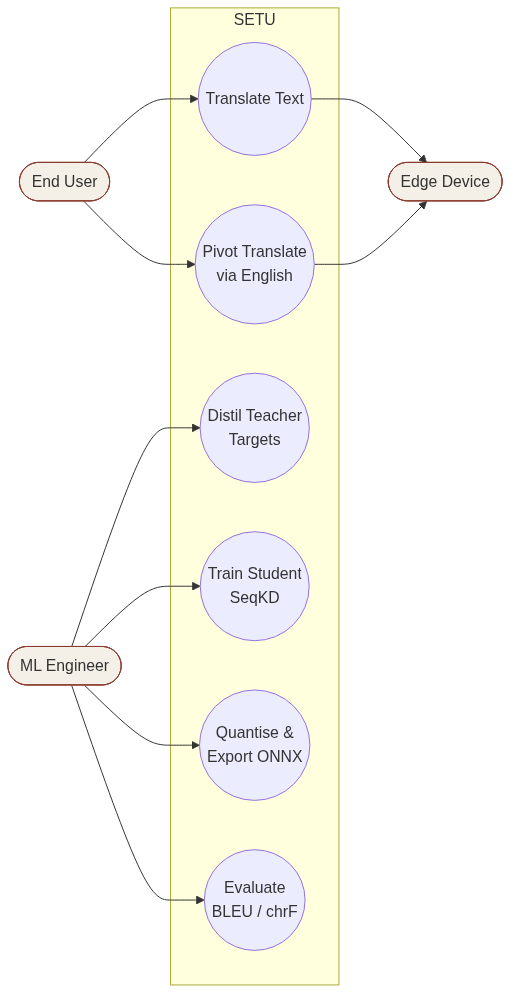
\includegraphics[width=\textwidth, height=0.88\textheight, keepaspectratio]{figures/use_case.png}
\caption{Use case diagram: End User, ML Engineer and Edge Device actors}
\label{fig:usecase}
\end{figure}

\begin{table}[H]
\centering
\caption{Use case specifications}
\label{tab:usecases}
\begin{tabular}{@{}L{2.7cm} L{1.9cm} L{4.3cm} L{4.6cm}@{}}
\toprule
\rowcolor{headblue}
\textbf{Use case} & \textbf{Actor} & \textbf{Precondition} & \textbf{Postcondition} \\
\midrule
Translate Text & End User & A trained model exists for the requested direction & Translated text returned with measured latency \\
\rowcolor{rowgrey}
Pivot Translate & End User & No direct model exists, but both source\arrowto{}English and English\arrowto{}target models exist & Translated text returned, flagged \texttt{pivot="en"} \\
List Languages & End User & Language registry loaded & 22 scheduled languages plus English returned, trained ones marked \\
\rowcolor{rowgrey}
Distil Teacher Targets & ML Engineer & Cleaned corpus available; teacher checkpoint reachable & Distilled corpus of teacher one-best targets written \\
Train Student & ML Engineer & Distilled corpus available; GPU available & Trained checkpoint plus a training report written \\
\rowcolor{rowgrey}
Quantise \& Export & ML Engineer & Trained checkpoint exists & INT8 and INT4 ONNX artifacts with a quantisation report \\
Evaluate & ML Engineer & Student and teacher both available & BLEU, chrF and student/teacher ratio recorded \\
\rowcolor{rowgrey}
Execute Inference & Edge Device & Quantised model and tokenizer present locally & Translation produced with zero network calls \\
\bottomrule
\end{tabular}
\end{table}

\subsection{Sequence Diagram}
\label{subsec:sequence}

Figure~\ref{fig:sequence} traces a single translation request. The significant
branch is the pivot: when a directly trained model exists the engine performs
one hop, and when it does not (every Indic-to-Indic pair) the engine
performs two, passing the intermediate English string from the first student to
the second. The response carries the summed latency of both hops and a
\texttt{pivot} field so that the caller can tell the two cases apart.

\begin{figure}[H]
\centering
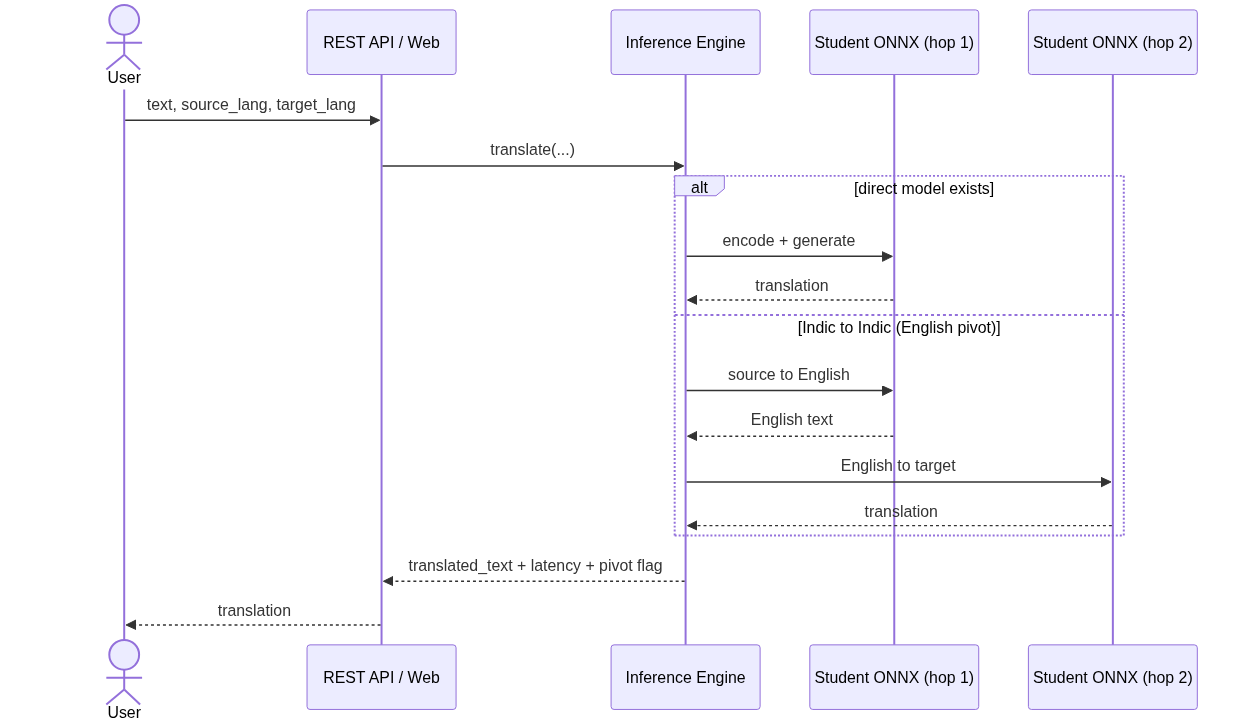
\includegraphics[width=\textwidth, height=0.80\textheight, keepaspectratio]{figures/sequence.png}
\caption{Sequence diagram: direct translation and the two-hop English pivot}
\label{fig:sequence}
\end{figure}

\subsection{Activity Diagram}
\label{subsec:activity}

Figure~\ref{fig:activity} shows the full training and deployment activity flow.
Everything above the dividing line executes once per direction on a GPU;
everything below executes on the user's device. The two decision points are the
quality gate (does the student reach 80\,\% of teacher BLEU) and the
routing decision at inference time.

\begin{figure}[H]
\centering
\scalebox{0.84}{%
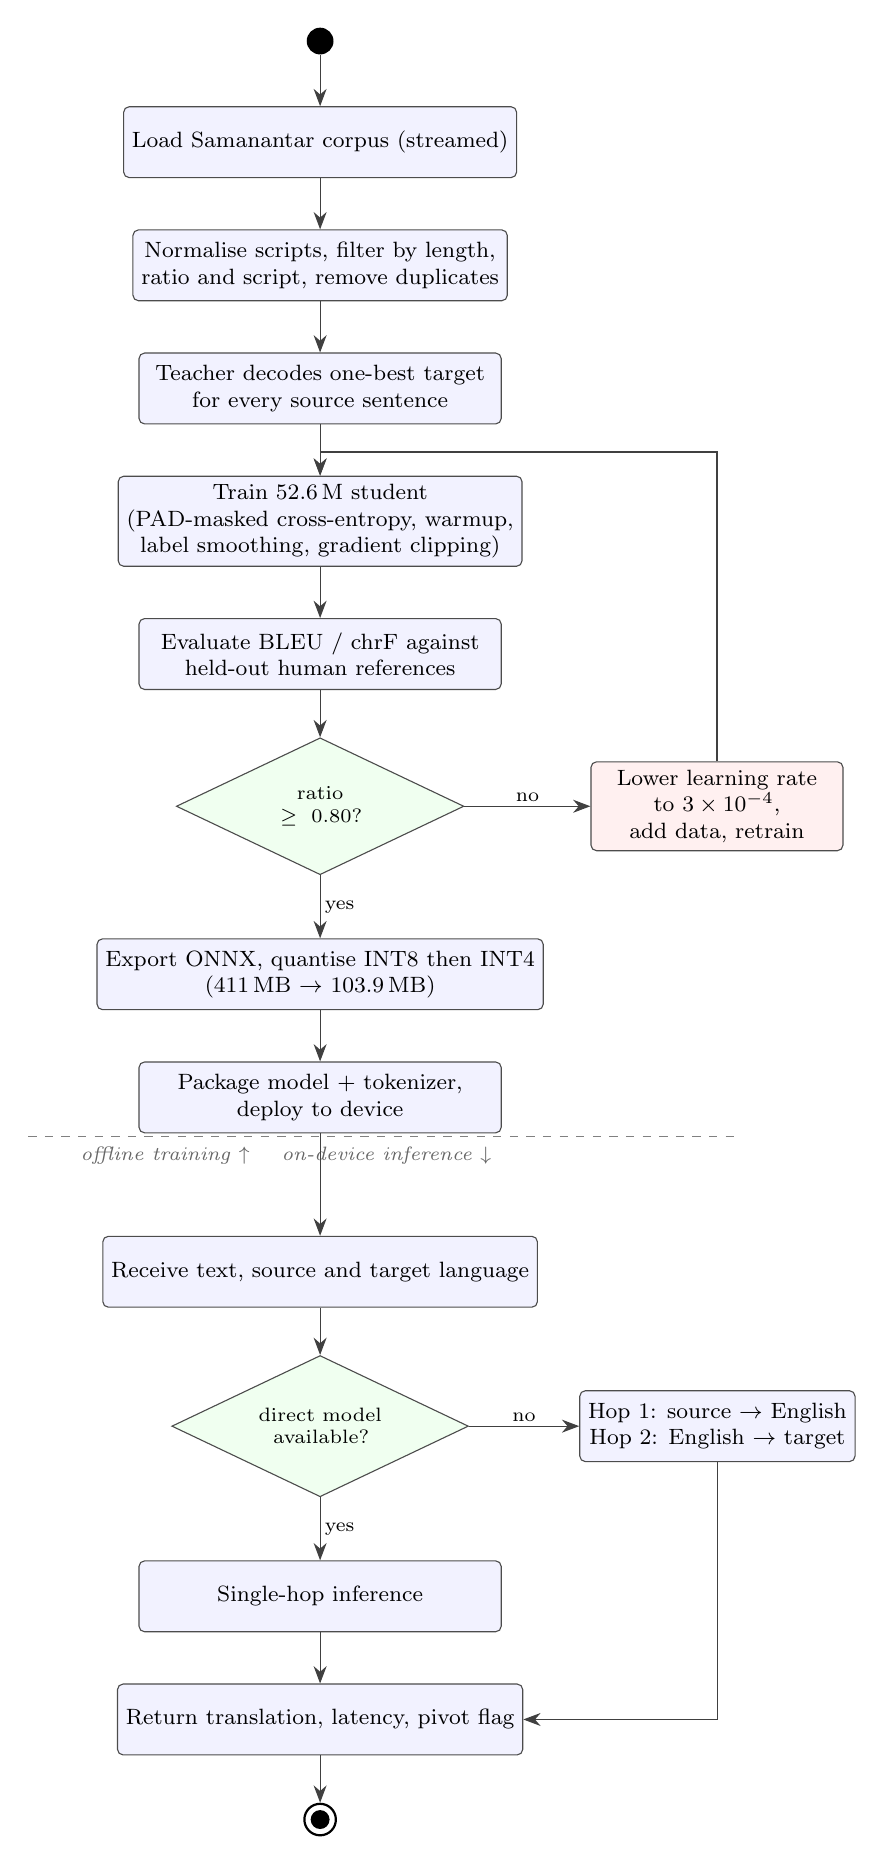
\begin{tikzpicture}[node distance=6.5mm and 9mm]
  \node[circle, fill=black, minimum size=3.4mm, inner sep=0] (start) {};
  \node[proc, below=of start, minimum width=46mm] (load)  {Load Samanantar corpus (streamed)};
  \node[proc, below=of load, minimum width=46mm]  (clean) {Normalise scripts, filter by length,\\ratio and script, remove duplicates};
  \node[proc, below=of clean, minimum width=46mm] (teach) {Teacher decodes one-best target\\for every source sentence};
  \node[proc, below=of teach, minimum width=46mm] (train) {Train 52.6\,M student\\(PAD-masked cross-entropy, warmup,\\label smoothing, gradient clipping)};
  \node[proc, below=of train, minimum width=46mm] (eval)  {Evaluate BLEU / chrF against\\held-out human references};
  \node[dec,  below=6mm of eval, text width=24mm] (gate)  {ratio\\$\geq 0.80$?};
  \node[proc, right=16mm of gate, minimum width=32mm, fill=red!6] (retune) {Lower learning rate\\to $3\times10^{-4}$,\\add data, retrain};
  \node[proc, below=8mm of gate, minimum width=46mm] (quant) {Export ONNX, quantise INT8 then INT4\\(411\,MB $\rightarrow$ 103.9\,MB)};
  \node[proc, below=of quant, minimum width=46mm] (ship)  {Package model + tokenizer,\\deploy to device};

  \draw[fl] (start) -- (load);
  \draw[fl] (load)  -- (clean);
  \draw[fl] (clean) -- (teach);
  \draw[fl] (teach) -- (train);
  \draw[fl] (train) -- (eval);
  \draw[fl] (eval)  -- (gate);
  \draw[fl] (gate)  -- node[lbl,above]{no} (retune);
  \draw[fl] (retune.north) |- ([yshift=3mm]train.north) -- (train.north);
  \draw[fl] (gate)  -- node[lbl,right]{yes} (quant);
  \draw[fl] (quant) -- (ship);

  \draw[dashed, black!50] ([xshift=-14mm,yshift=-5mm]ship.west) -- ([xshift=30mm,yshift=-5mm]ship.east)
        node[pos=0.06, below, font=\scriptsize\itshape, black!60, anchor=north west]
        {offline training $\uparrow$ \quad on-device inference $\downarrow$};

  \node[proc, below=13mm of ship, minimum width=46mm] (req)  {Receive text, source and target language};
  \node[dec,  below=6mm of req, text width=26mm] (direct) {direct model\\available?};
  \node[proc, right=14mm of direct, minimum width=32mm] (pivot) {Hop 1: source $\rightarrow$ English\\Hop 2: English $\rightarrow$ target};
  \node[proc, below=8mm of direct, minimum width=46mm] (single) {Single-hop inference};
  \node[proc, below=of single, minimum width=46mm] (out) {Return translation, latency, pivot flag};
  \node[circle, draw=black, thick, minimum size=4mm, inner sep=0, below=6mm of out] (endo) {};
  \node[circle, fill=black, minimum size=2.4mm, inner sep=0] at (endo) {};

  \draw[fl] (ship) -- (req);
  \draw[fl] (req)  -- (direct);
  \draw[fl] (direct) -- node[lbl,above]{no} (pivot);
  \draw[fl] (direct) -- node[lbl,right]{yes} (single);
  \draw[fl] (pivot.south) |- (out.east);
  \draw[fl] (single) -- (out);
  \draw[fl] (out) -- (endo);
\end{tikzpicture}}
\caption{Activity diagram: offline training pipeline (above) and on-device inference (below)}
\label{fig:activity}
\end{figure}

\subsection{State Chart Diagram}
\label{subsec:statechart}

A model in \setu{} passes through a well-defined sequence of states.
Figure~\ref{fig:statechart} records them, including the two transitions that
were exercised in practice: the collapse detected at evaluation and the recovery
achieved by retraining at a lower learning rate on the same distilled corpus.

\begin{figure}[H]
\centering
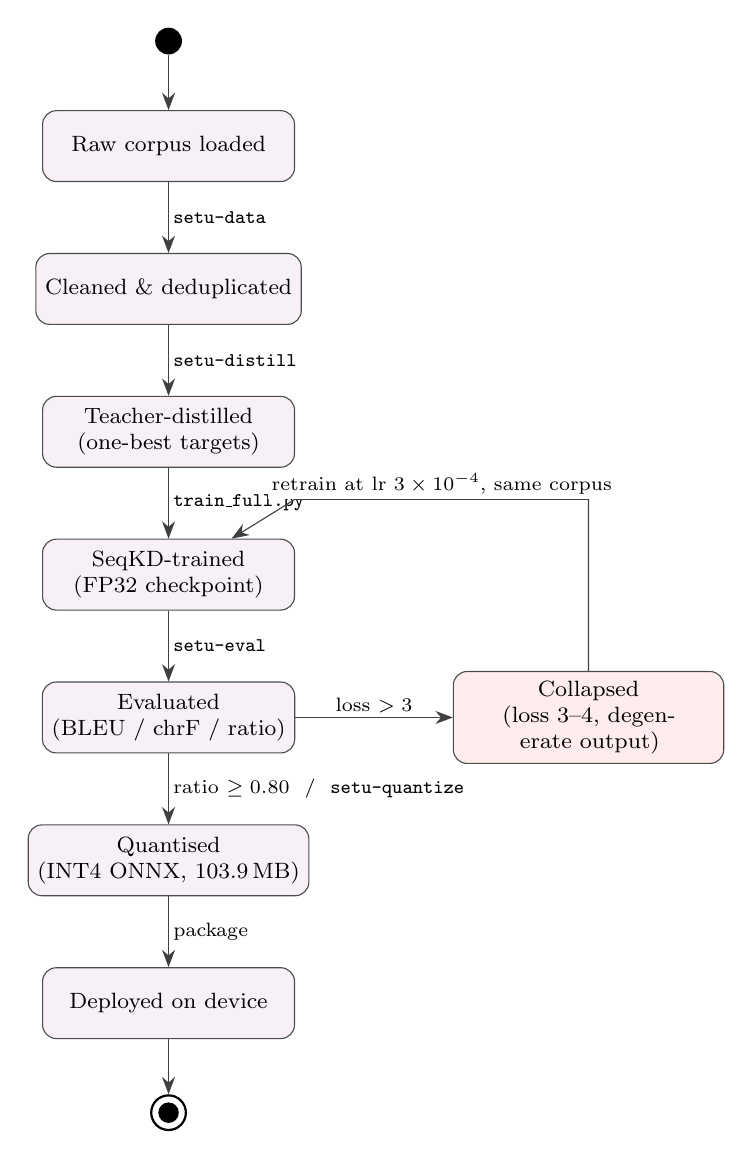
\begin{tikzpicture}[node distance=9mm and 20mm]
  \node[circle, fill=black, minimum size=3.4mm, inner sep=0] (i) {};
  \node[st, below=7mm of i]      (raw)   {Raw corpus loaded};
  \node[st, below=of raw]        (clean) {Cleaned \& deduplicated};
  \node[st, below=of clean]      (dist)  {Teacher-distilled\\(one-best targets)};
  \node[st, below=of dist]       (trn)   {\seqkd{}-trained\\(FP32 checkpoint)};
  \node[st, below=of trn]        (evl)   {Evaluated\\(BLEU / chrF / ratio)};
  \node[st, below=of evl]        (qnt)   {Quantised\\(INT4 ONNX, 103.9\,MB)};
  \node[st, below=of qnt]        (dep)   {Deployed on device};
  \node[circle, draw=black, thick, minimum size=4.4mm, inner sep=0, below=7mm of dep] (f) {};
  \node[circle, fill=black, minimum size=2.6mm, inner sep=0] at (f) {};

  \node[st, right=of evl, fill=red!7, text width=32mm] (col) {Collapsed\\(loss 3--4, degenerate output)};

  \draw[fl] (i)     -- (raw);
  \draw[fl] (raw)   -- node[lbl,right]{\texttt{setu-data}} (clean);
  \draw[fl] (clean) -- node[lbl,right]{\texttt{setu-distill}} (dist);
  \draw[fl] (dist)  -- node[lbl,right]{\texttt{train\_full.py}} (trn);
  \draw[fl] (trn)   -- node[lbl,right]{\texttt{setu-eval}} (evl);
  \draw[fl] (evl)   -- node[lbl,right]{ratio $\geq 0.80$ \ / \ \texttt{setu-quantize}} (qnt);
  \draw[fl] (qnt)   -- node[lbl,right]{package} (dep);
  \draw[fl] (dep)   -- (f);

  \draw[fl] (evl) -- node[lbl,above]{loss $>3$} (col);
  \draw[fl] (col.north) |- node[lbl,pos=0.75,above]{retrain at lr $3\times10^{-4}$, same corpus} ([yshift=5mm]trn.north east) -- ([xshift=8mm]trn.north);
\end{tikzpicture}
\caption{State chart diagram: model lifecycle from raw corpus to deployed artifact, including the observed collapse and recovery transitions}
\label{fig:statechart}
\end{figure}

\subsection{Data Flow Diagram}
\label{subsec:dfd}

% \begin{landscape} forces a page break, and the last line of this paragraph was
% spilling onto an otherwise blank page ahead of it. One extra line on the
% previous page keeps the paragraph whole.
\enlargethispage{\baselineskip}
Figure~\ref{fig:dfd} gives the level-1 data flow. The corpus is an external
data source; the teacher is a transformation that produces the distilled data
store; the trainer consumes that store and produces a student; the quantiser
converts the student into a deployable artifact; the inference engine consumes
the artifact and produces translations. The evaluator is a side branch that
consumes both student and teacher outputs to compute the ratio that gates
deployment.

% Aspect ratio 9.74, the widest diagram in the report: sideways page.
\widefigure{width=\linewidth, keepaspectratio}{figures/data_flow.png}%
  {Level-1 data flow diagram: corpus to deployed translation}{fig:dfd}

\subsection{Entity-Relationship Model}
\label{subsec:er}

\setu{} does not use a relational database (an offline edge deployment should
not require one), but its persistent artifacts have a clear relational
structure, recorded in Figure~\ref{fig:er}. Corpora are stored as JSONL,
reports as JSON, models as ONNX with an accompanying SentencePiece tokenizer,
and the language registry as YAML.

\begin{figure}[H]
\centering
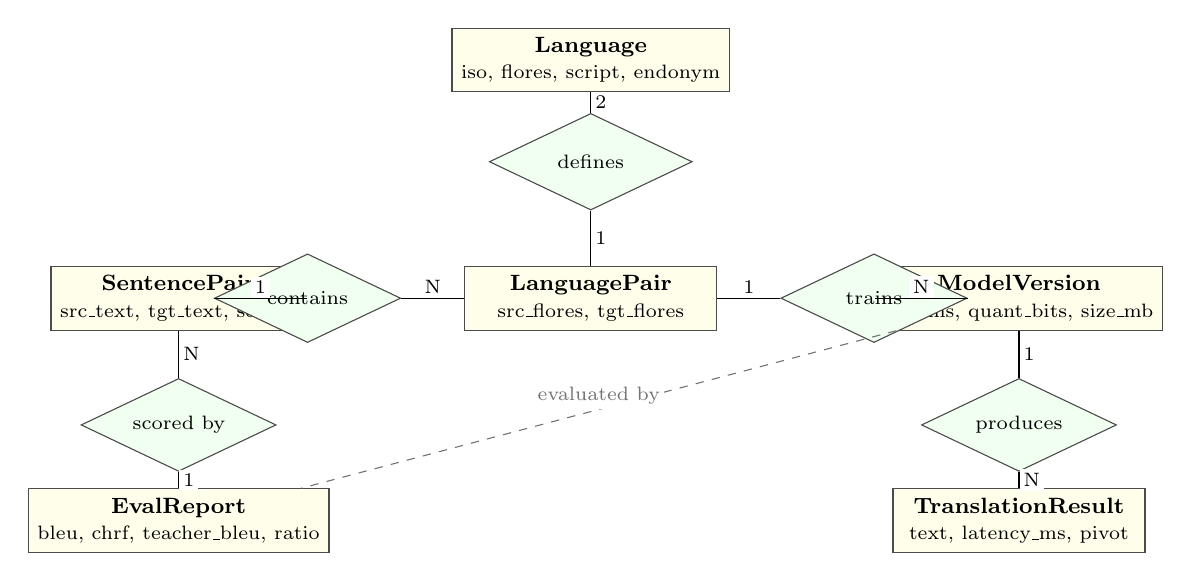
\begin{tikzpicture}[node distance=13mm and 20mm]
  \node[ent, minimum width=30mm] (lang) {\textbf{Language}\\\scriptsize iso, flores, script, endonym};
  \node[ent, below=22mm of lang, minimum width=32mm] (pair) {\textbf{LanguagePair}\\\scriptsize src\_flores, tgt\_flores};
  \node[ent, left=of pair, minimum width=30mm] (sent) {\textbf{SentencePair}\\\scriptsize src\_text, tgt\_text, source};
  \node[ent, right=of pair, minimum width=32mm] (mv) {\textbf{ModelVersion}\\\scriptsize params, quant\_bits, size\_mb};
  \node[ent, below=20mm of sent, minimum width=32mm] (ev) {\textbf{EvalReport}\\\scriptsize bleu, chrf, teacher\_bleu, ratio};
  \node[ent, below=20mm of mv, minimum width=32mm] (tr) {\textbf{TranslationResult}\\\scriptsize text, latency\_ms, pivot};

  \node[dec, above=7mm of pair, text width=20mm] (has) {defines};
  \node[dec, left=6mm of pair, text width=18mm, xshift=-2mm] (cont) {contains};
  \node[dec, right=6mm of pair, text width=18mm, xshift=2mm] (trained) {trains};
  \node[dec, below=6mm of sent, text width=18mm] (scored) {scored by};
  \node[dec, below=6mm of mv, text width=18mm] (prod) {produces};

  \draw[-] (lang) -- node[lbl,right]{2} (has);
  \draw[-] (has)  -- node[lbl,right]{1} (pair);
  \draw[-] (pair) -- node[lbl,above]{N} (cont);
  \draw[-] (cont) -- node[lbl,above]{1} (sent);
  \draw[-] (pair) -- node[lbl,above]{1} (trained);
  \draw[-] (trained) -- node[lbl,above]{N} (mv);
  \draw[-] (sent) -- node[lbl,right]{N} (scored);
  \draw[-] (scored) -- node[lbl,right]{1} (ev);
  \draw[-] (mv)   -- node[lbl,right]{1} (prod);
  \draw[-] (prod) -- node[lbl,right]{N} (tr);
  \draw[-, dashed, black!55] (mv) -- node[lbl,above,pos=0.5]{evaluated by} (ev);
\end{tikzpicture}
\caption{Entity-relationship model of \setu{}'s persistent artifacts}
\label{fig:er}
\end{figure}

\subsection{Class Diagram}
\label{subsec:class}

Figure~\ref{fig:class} gives the principal classes. The design deliberately
isolates every dependency on the teacher's implementation inside a single class,
\texttt{IndicTrans2Teacher}. A unit test scans the source tree and fails the
build if any other module imports \texttt{transformers}, \texttt{torch} or
\texttt{IndicTransToolkit}. This is what allows the deployed artifact to contain
no training dependencies at all.

\begin{figure}[H]
\centering
\scalebox{0.97}{%
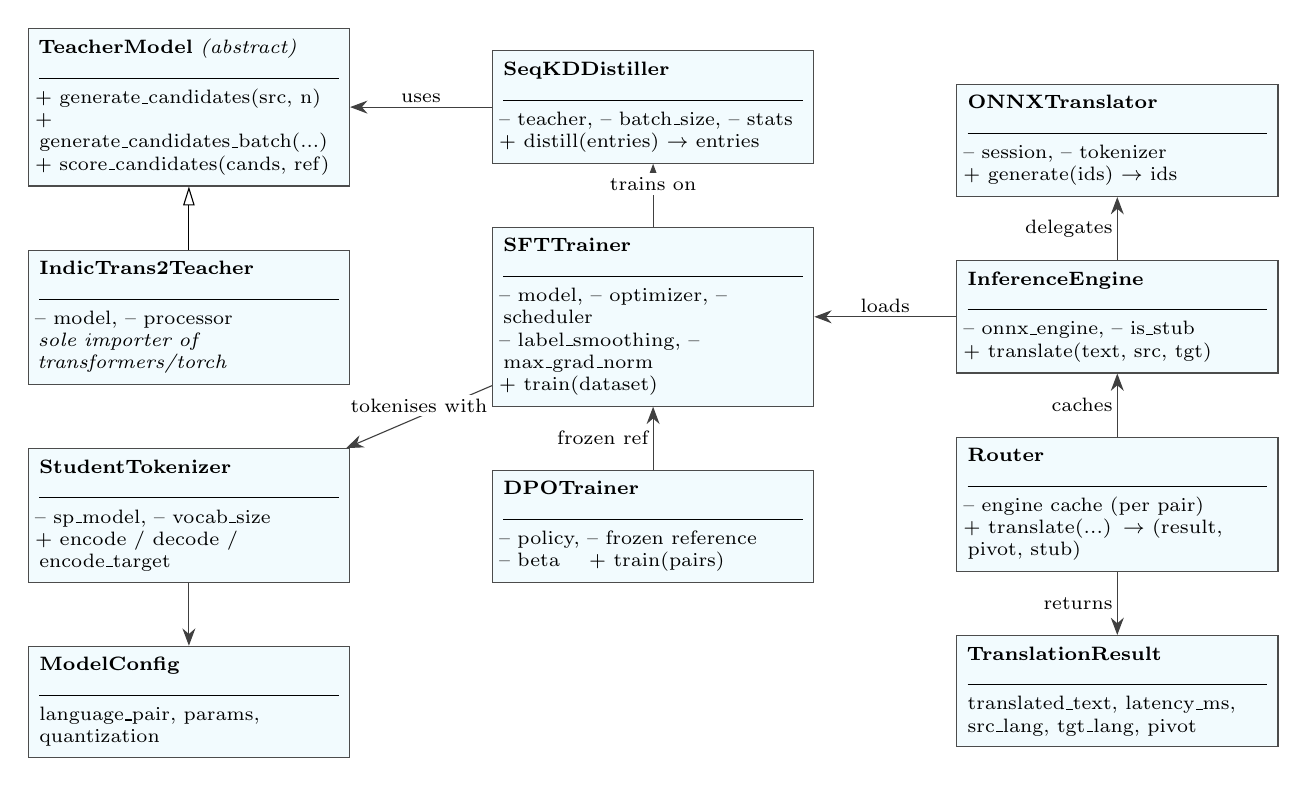
\begin{tikzpicture}[node distance=8mm and 10mm]
  \node[cls] (teacher) {%
    \textbf{TeacherModel} \textit{(abstract)}\clsrule + generate\_candidates(src, n)\\
    + generate\_candidates\_batch(...)\\
    + score\_candidates(cands, ref)};
  \node[cls, below=of teacher] (it2) {%
    \textbf{IndicTrans2Teacher}\clsrule -- model, -- processor\\
    \textit{sole importer of transformers/torch}};
  \node[cls, right=18mm of teacher] (dist) {%
    \textbf{SeqKDDistiller}\clsrule -- teacher, -- batch\_size, -- stats\\
    + distill(entries) $\rightarrow$ entries};
  \node[cls, below=of dist] (sft) {%
    \textbf{SFTTrainer}\clsrule -- model, -- optimizer, -- scheduler\\
    -- label\_smoothing, -- max\_grad\_norm\\
    + train(dataset)};
  \node[cls, below=of sft] (dpo) {%
    \textbf{DPOTrainer}\clsrule -- policy, -- frozen reference\\
    -- beta \quad + train(pairs)};
  \node[cls, below=of it2] (tok) {%
    \textbf{StudentTokenizer}\clsrule -- sp\_model, -- vocab\_size\\
    + encode / decode / encode\_target};
  \node[cls, below=of tok] (cfg) {%
    \textbf{ModelConfig}\clsrule language\_pair, params,\\quantization};
  \node[cls, right=18mm of sft] (eng) {%
    \textbf{InferenceEngine}\clsrule -- onnx\_engine, -- is\_stub\\
    + translate(text, src, tgt)};
  \node[cls, above=of eng] (onnx) {%
    \textbf{ONNXTranslator}\clsrule -- session, -- tokenizer\\
    + generate(ids) $\rightarrow$ ids};
  \node[cls, below=of eng] (router) {%
    \textbf{Router}\clsrule -- engine cache (per pair)\\
    + translate(...) $\rightarrow$ (result, pivot, stub)};
  \node[cls, below=of router] (res) {%
    \textbf{TranslationResult}\clsrule translated\_text, latency\_ms,\\src\_lang, tgt\_lang, pivot};

  \draw[-{Triangle[open, length=2.4mm]}] (it2) -- (teacher);
  \draw[fl] (dist) -- node[lbl,above]{uses} (teacher);
  \draw[fl] (sft)  -- node[lbl,above]{trains on} (dist);
  \draw[fl] (dpo)  -- node[lbl,left]{frozen ref} (sft);
  \draw[fl] (sft)  -- node[lbl,above]{tokenises with} (tok);
  \draw[fl] (tok)  -- (cfg);
  \draw[fl] (eng)  -- node[lbl,left]{delegates} (onnx);
  \draw[fl] (router) -- node[lbl,left]{caches} (eng);
  \draw[fl] (router) -- node[lbl,left]{returns} (res);
  \draw[fl] (eng)  -- node[lbl,above]{loads} (sft);
\end{tikzpicture}}
\caption{Class diagram: training classes (left) are used offline by the ML Engineer; inference classes (right) ship to the device}
\label{fig:class}
\end{figure}

\needspace{16\baselineskip}
\section{Software Requirements Specification}
\label{sec:srs}

This section states what the system must do, independently of how it does it.

\subsection{User Requirements}
\label{subsec:userreq}

\begin{table}[H]
\centering
\caption{User requirements}
\label{tab:userreq}
\begin{tabular}{@{}L{1.4cm} L{2.6cm} J{9.8cm}@{}}
\toprule
\rowcolor{headblue}
\textbf{ID} & \textbf{User} & \textbf{Requirement} \\
\midrule
UR-1 & End user & Translate text between any two supported languages without an internet connection \\
\rowcolor{rowgrey}
UR-2 & End user & See which languages are available and which are not yet trained, before attempting a translation \\
UR-3 & End user & Receive a translation quickly enough for conversational use \\
\rowcolor{rowgrey}
UR-4 & End user & Be assured that the text typed never leaves the device \\
UR-5 & End user & Use the system from a browser, a mobile application, a command line or a programmatic API, with identical behaviour \\
\rowcolor{rowgrey}
UR-6 & ML engineer & Train a model for any language pair by changing configuration, without modifying source code \\
UR-7 & ML engineer & Resume a multi-hour training run after a disconnection without repeating completed stages \\
\rowcolor{rowgrey}
UR-8 & ML engineer & Obtain an honest quality report, including failure, rather than an optimistic one \\
UR-9 & Deployer & Install models on a fresh machine and run the system without training anything \\
\bottomrule
\end{tabular}
\end{table}

\subsection{System Requirements}
\label{subsec:sysreq}

\begin{itemize}
  \item \textbf{SR-1.} Python 3.11 or 3.12; Python 3.14 is incompatible with the
        teacher's remote modelling code.
  \item \textbf{SR-2.} \texttt{transformers} at least 4.42 and below 4.54, since
        4.54 removed the legacy tuple \texttt{past\_key\_values} cache API that
        the rotary teacher relies on.
  \item \textbf{SR-3.} PyTorch 2.6 or newer for training, paired with a matching
        \texttt{torchvision} build.
  \item \textbf{SR-4.} ONNX Runtime with the CPU execution provider for
        inference; no GPU dependency in the deployed artifact.
  \item \textbf{SR-5.} A CUDA-capable GPU with at least 16\,GB of memory for
        training a direction.
  \item \textbf{SR-6.} At least 104\,MB of free storage per translation
        direction on the target device.
  \item \textbf{SR-7.} Node.js 18 or newer to build the browser client (build
        time only; the exported application is static).
\end{itemize}

\subsection{Functional Requirements}
\label{subsec:funcreq}

\begin{longtable}{@{}L{1.4cm} J{7.8cm} L{4.6cm}@{}}
\caption{Functional requirements}
\label{tab:funcreq}\\
\toprule
\rowcolor{headblue}
\textbf{ID} & \textbf{Requirement} & \textbf{Verified by} \\
\midrule
\endfirsthead
\multicolumn{3}{c}{\textit{Table \thetable{} (continued)}}\\
\toprule
\rowcolor{headblue}
\textbf{ID} & \textbf{Requirement} & \textbf{Verified by} \\
\midrule
\endhead
\midrule
\multicolumn{3}{r}{\textit{continued on next page}}\\
\endfoot
\bottomrule
\endlastfoot

FR-1 & Translate text between supported Indian languages and English in both directions, fully offline & \S\ref{subsec:unittest}, \S\ref{sec:testreports} \\
\rowcolor{rowgrey}
FR-2 & Accept plain-text input of up to 512 tokens per request & \S\ref{subsec:unittest} \\
FR-3 & Reject a request whose source and target language are identical & UT-2 \\
\rowcolor{rowgrey}
FR-4 & Reject a request containing an unknown language code & UT-3 \\
FR-5 & Route Indic-to-Indic pairs through English when no direct model exists, and report that it did so & IT-1 to IT-3 \\
\rowcolor{rowgrey}
FR-6 & Expose \texttt{POST /translate}, \texttt{GET /languages}, \texttt{GET /models} and \texttt{GET /health} & \S\ref{sec:interface}, IT-4 \\
FR-7 & Discover every model present on disk at start-up and report its variant and size & IT-4 \\
\rowcolor{rowgrey}
FR-8 & Generate teacher one-best targets for an arbitrary corpus slice & \S\ref{subsec:mod2} \\
FR-9 & Train a student on either distilled or reference targets, selectable at run time & \S\ref{subsec:mod3} \\
\rowcolor{rowgrey}
FR-10 & Quantise a trained student to INT8 and INT4 ONNX with a per-stage benchmark & \S\ref{subsec:mod4} \\
FR-11 & Report BLEU, chrF and the student/teacher ratio per direction & \S\ref{sec:testreports} \\
\rowcolor{rowgrey}
FR-12 & Support incremental addition of a language by configuration alone & \S\ref{subsec:mod8} \\
\end{longtable}

\subsection{Non-Functional Requirements}
\label{subsec:nonfuncreq}

\begin{table}[H]
\centering
\caption{Non-functional requirements and measured outcomes}
\label{tab:nonfuncreq}
\begin{tabular}{@{}L{1.3cm} L{3.0cm} L{4.4cm} L{5.0cm}@{}}
\toprule
\rowcolor{headblue}
\textbf{ID} & \textbf{Attribute} & \textbf{Requirement} & \textbf{Measured outcome} \\
\midrule
NFR-1 & Performance & Under 500\,ms per sentence on ARM-class CPU & Mean 105--202\,ms; p90 141--541\,ms (one outlier) \\
\rowcolor{rowgrey}
NFR-2 & Size & At most 200\,MB per direction after quantisation & 103.9\,MB for every direction \\
NFR-3 & Accuracy & At least 80\,\% of teacher BLEU & 14 of 22 directions; mean ratio 0.838 \\
\rowcolor{rowgrey}
NFR-4 & Availability & Fully functional offline after initial setup & Verified with all sockets disabled \\
NFR-5 & Privacy & No user text transmitted during inference & Verified by code audit and the offline test \\
\rowcolor{rowgrey}
NFR-6 & Portability & Runs on x86-64 and ARM, Linux and Android & ONNX Runtime CPU provider on both \\
NFR-7 & Maintainability & Single shared engine behind every interface & \texttt{setu.inference.router} \\
\rowcolor{rowgrey}
NFR-8 & Testability & Automated suite covering every module & 85 tests \\
NFR-9 & Reliability & Degrade explicitly, never silently & Stub engine reports \texttt{stub:true}; scorecard reports \textsc{unverified} without evidence \\
\bottomrule
\end{tabular}
\end{table}

\subsection{Domain Requirements}
\label{subsec:domainreq}

\begin{itemize}
  \item \textbf{DR-1.} Language identification must follow the script-qualified
        FLORES convention used by IndicTrans2 (\texttt{hin\_Deva},
        \texttt{eng\_Latn}), because several scheduled languages are written in
        more than one script. Kashmiri, Manipuri and Sindhi accordingly carry
        dual-script registry entries.
  \item \textbf{DR-2.} Script normalisation must preserve zero-width joiners and
        non-joiners, which are semantically significant in Indic scripts; naive
        control-character stripping corrupts valid text.
  \item \textbf{DR-3.} Corpus cleaning must enforce a minimum fraction of
        letters in the expected script, so that mined pairs with the wrong
        language on one side are removed.
  \item \textbf{DR-4.} Evaluation must always use real human references held out
        from training, never teacher output, regardless of what the student was
        trained on. This is what makes the comparison in
        Section~\ref{sec:headtohead} fair.
  \item \textbf{DR-5.} Tokenizer language tags must be reserved for all 22
        scheduled languages from the first training run, so that token
        identifiers remain stable when languages are added later and previously
        trained models need not be re-tokenised.
  \item \textbf{DR-6.} BLEU must not be compared across languages. Agglutinative
        languages such as Malayalam and Tamil score low in absolute BLEU for
        morphological reasons; only the student/teacher ratio is comparable
        across directions.
\end{itemize}

% ============================== CHAPTER 4 ===================================
\chapter{Project Planning}
\label{ch:planning}

Planning a machine learning systems project differs from planning conventional
software in one decisive respect: several tasks have durations that cannot be
known until they are attempted, and some have outcomes that determine which
tasks follow. Teacher distillation over half a million sentences takes as long
as it takes; a student either converges or collapses, and a collapse adds an
unplanned diagnostic and retraining cycle. The plan described here was therefore
built around milestones with explicit evidence requirements rather than around
fixed-duration activities, and it carried deliberate slack on the training
tasks.

This chapter presents the work breakdown structure, the schedule as a Gantt
chart across both project phases, a PERT analysis with the critical path, the
risk register with the mitigations actually applied, and the division of
responsibility within the team.

\section{Project Planning and Scheduling}
\label{sec:planning}

\subsection{Work Breakdown Structure}
\label{subsec:wbs}

The project decomposes into nine engineering milestones, M0 through M8, followed
by a hardening and delivery milestone. Each milestone is a single commit with a
defined completion criterion, so that progress is verifiable rather than
self-reported. Table~\ref{tab:wbs} gives the breakdown together with the
evidence required to close each item.

\begin{longtable}{@{}L{1.1cm} L{3.5cm} L{5.4cm} L{4.1cm}@{}}
\caption{Work breakdown structure with completion evidence}
\label{tab:wbs}\\
\toprule
\rowcolor{headblue}
\textbf{ID} & \textbf{Task} & \textbf{Description} & \textbf{Completion evidence} \\
\midrule
\endfirsthead
\multicolumn{4}{c}{\textit{Table \thetable{} (continued)}}\\
\toprule
\rowcolor{headblue}
\textbf{ID} & \textbf{Task} & \textbf{Description} & \textbf{Completion evidence} \\
\midrule
\endhead
\midrule
\multicolumn{4}{r}{\textit{continued on next page}}\\
\endfoot
\bottomrule
\endlastfoot

M0 & Scaffold & Package layout, four core data objects, YAML configuration with the 22-language registry, CLI, passthrough stub engine & 7 tests green; CLI runs end to end \\
\rowcolor{rowgrey}
M1 & Data pipeline & Corpus loading, script normalisation, length and script filtering, deduplication, JSONL output & 50{,}000 pairs in, 49{,}520 clean pairs out, with a filter breakdown report \\
M2 & Teacher integration & IndicTrans2 behind an abstract interface; a test forbids any other module importing the teacher's dependencies & Real smoke test producing fluent candidate translations \\
\rowcolor{rowgrey}
M3 & Preference generation & Teacher $n$-best candidates plus $k$-NN retrieved neighbours, chrF ranking, pair validation & 500 entries $\rightarrow$ 3{,}494 candidates $\rightarrow$ 2{,}074 validated pairs \\
M4 & SFT and DPO training & SentencePiece tokenizer, student model, supervised fine-tuning, DPO with a frozen reference, evaluation harness & DPO measurably outperforms SFT; test enforces the reference stays frozen \\
\rowcolor{rowgrey}
M5 & Quantisation and offline inference & ONNX export, progressive INT8 and INT4 quantisation, ONNX inference engine, socket-disabling offline assertion & Size, latency and offline targets all pass \\
M6 & Interfaces & FastAPI REST service, CLI, offline PWA, mobile SDK stubs, all sharing one engine & 15 interface tests green \\
\rowcolor{rowgrey}
M7 & All-in-One KD & Temperature-sampled cross-lingual balancing with a coverage report & Mechanism proven by test \\
M8 & Elastic Weight Consolidation & Diagonal-Fisher penalty, old-task snapshot, EWC training step & Measured retention of the old task above naive fine-tuning \\
\rowcolor{rowgrey}
M9 & Hardening and delivery & Scorecard generator, benchmarks, documentation, dead-code removal & Full suite green; scorecard reports \textsc{unverified} when evidence is absent \\
\midrule
P2-A & \seqkd{} baseline and head-to-head & Distiller CLI, \texttt{-{}-train-corpus} switch, S0/S1/S2/S3 comparison & Table~\ref{tab:h1} filled \\
\rowcolor{rowgrey}
P2-B & GPU campaign & Environment fixes, resumable runners, 22 directions trained bidirectionally & 22 per-direction reports \\
P2-C & Collapse diagnosis and recovery & Root-cause the two degenerate students and retrain & Both recovered to passing ratios \\
\rowcolor{rowgrey}
P2-D & English-pivot routing & Shared router used by REST and CLI alike & Verified on Hindi--Bengali, Tamil--Telugu, Assamese--Bengali \\
P2-E & Frontend and release & Next.js client, offline PWA, public model release, quick-start documentation & Live demo; models downloadable without login \\
\rowcolor{rowgrey}
P2-F & Report and paper & This report; paper plan with filled result tables & Submitted \\

\end{longtable}

\subsection{Gantt Chart}
\label{subsec:gantt}

Figure~\ref{fig:gantt} gives the schedule. Phase~1 ran from January to
mid-August 2026 and delivered the pipeline, the empirical finding and eleven
languages. Phase~2 runs from August to the end of October 2026 and covers the
remaining languages, benchmark rescoring, edge packaging and the final report.

% Redrawn in TikZ. The exported PNG was 2384x460 px, so even on a sideways page
% it rendered 4.6 cm tall with unreadable task labels. Drawn natively the task
% names sit at full size and the month axis is explicit.
\begin{landscape}
\vspace*{\fill}
\begin{figure}[H]
\centering
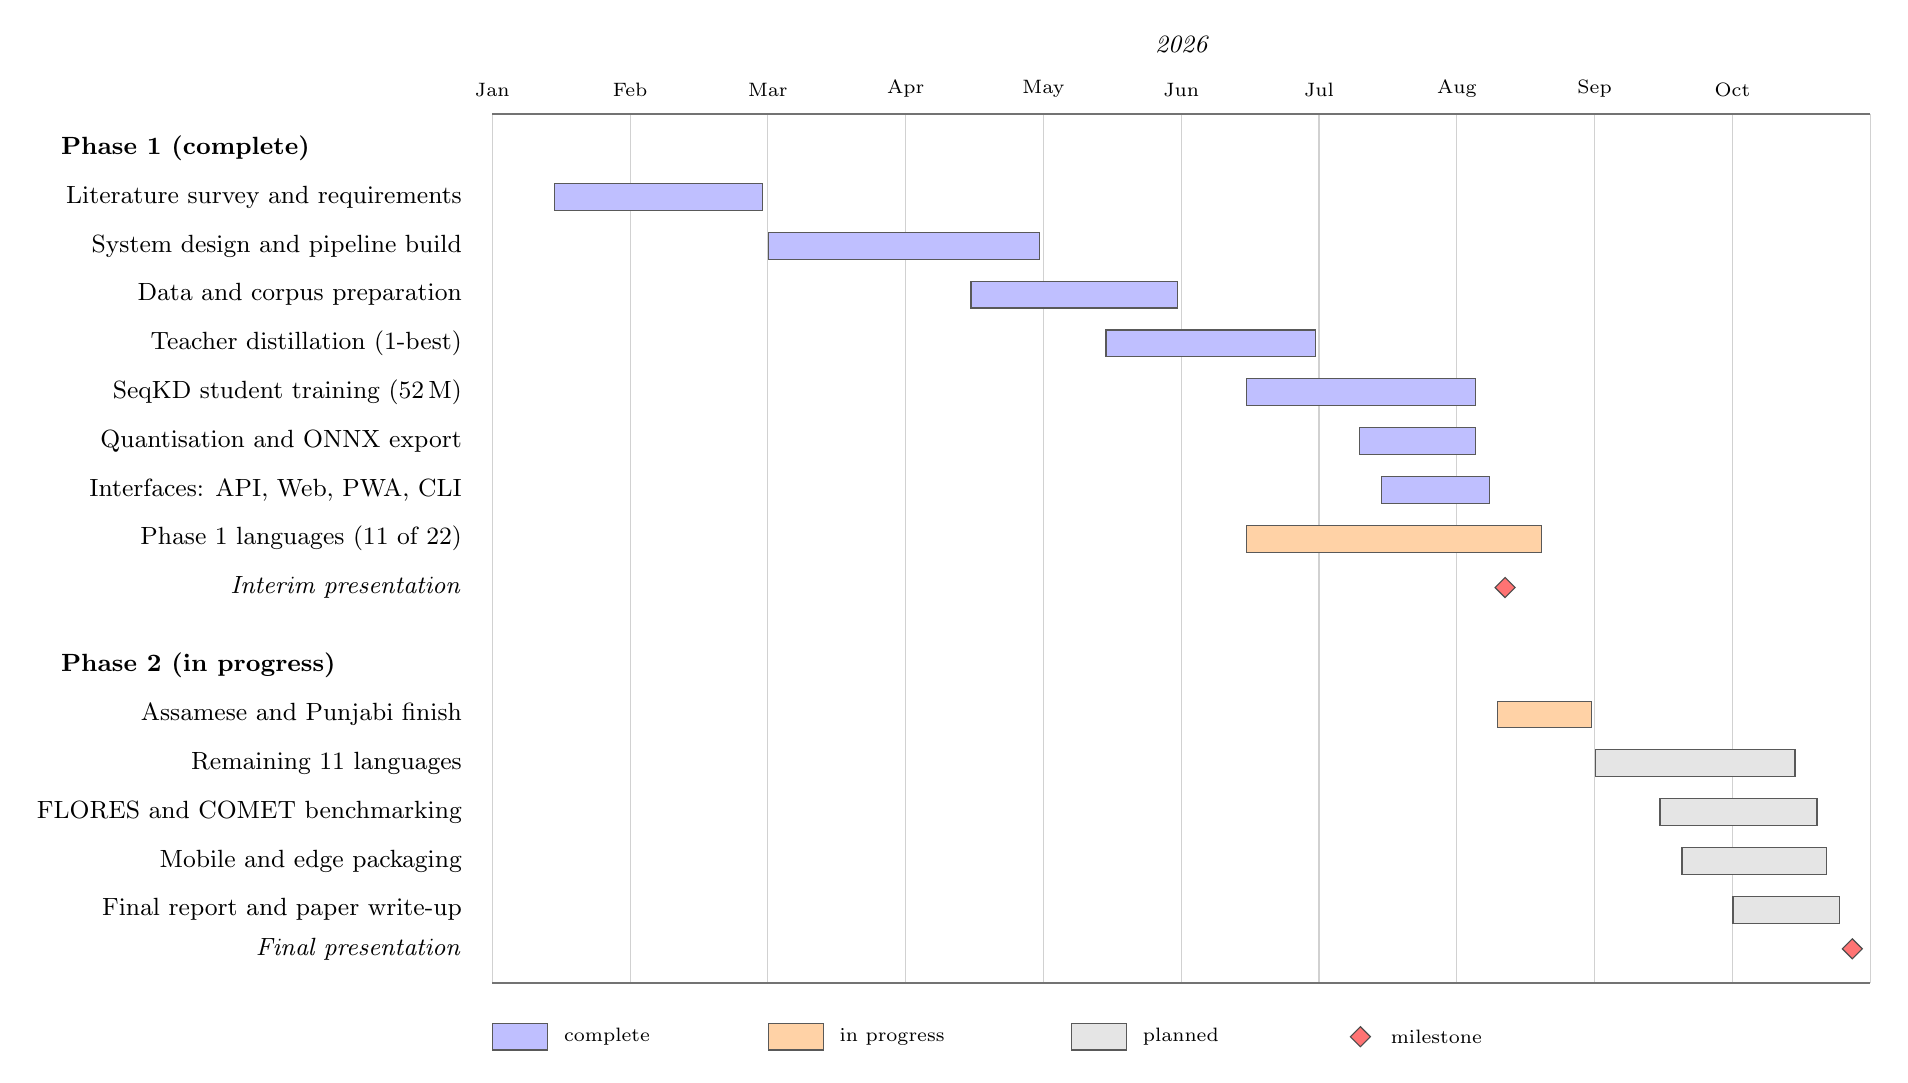
\begin{tikzpicture}[x=1.75cm, y=-0.62cm,
   bar/.style   = {draw=black!65, fill=blue!25, minimum height=3.4mm, inner sep=0pt},
   act/.style   = {draw=black!65, fill=orange!35, minimum height=3.4mm, inner sep=0pt},
   todo/.style  = {draw=black!65, fill=black!10, minimum height=3.4mm, inner sep=0pt},
   lab/.style   = {font=\small, anchor=east},
   sec/.style   = {font=\small\bfseries, anchor=west},
   ax/.style    = {font=\scriptsize, anchor=south}]

  \def\L{-0.15}                                  % right edge of the label column
  % month grid and axis
  \foreach \m/\n in {0/Jan,1/Feb,2/Mar,3/Apr,4/May,5/Jun,6/Jul,7/Aug,8/Sep,9/Oct,10/{}} {
     \draw[black!18] (\m,0.3) -- (\m,18.1);
     \node[ax] at (\m,0.15) {\n};
  }
  \draw[black!55] (0,0.3)  -- (10,0.3);
  \draw[black!55] (0,18.1) -- (10,18.1);
  \node[font=\small\itshape, anchor=south] at (5,-0.75) {2026};

  % ---- Phase 1 -------------------------------------------------------------
  \node[sec] at (\L-3.05,1) {Phase 1 (complete)};
  \foreach \r/\a/\b/\name in {%
      2/0.45/1.96/{Literature survey and requirements},
      3/2.00/3.97/{System design and pipeline build},
      4/3.47/4.97/{Data and corpus preparation},
      5/4.45/5.97/{Teacher distillation (1-best)},
      6/5.47/7.13/{SeqKD student training (52\,M)},
      7/6.29/7.13/{Quantisation and ONNX export},
      8/6.45/7.23/{Interfaces: API, Web, PWA, CLI}} {
     \node[lab] at (\L,\r) {\name};
     \node[bar, anchor=west, minimum width={(\b-\a)*1.75cm}] at (\a,\r) {};
  }
  \node[lab] at (\L,9) {Phase 1 languages (11 of 22)};
  \node[act, anchor=west, minimum width={(7.61-5.47)*1.75cm}] at (5.47,9) {};
  \node[lab] at (\L,10) {\textit{Interim presentation}};
  \node[diamond, draw=black!70, fill=red!55, minimum size=2.6mm, inner sep=0pt] at (7.35,10) {};

  % ---- Phase 2 -------------------------------------------------------------
  \node[sec] at (\L-3.05,11.6) {Phase 2 (in progress)};
  \node[lab] at (\L,12.6) {Assamese and Punjabi finish};
  \node[act, anchor=west, minimum width={(7.97-7.29)*1.75cm}] at (7.29,12.6) {};
  \foreach \r/\a/\b/\name in {%
      13.6/8.00/9.45/{Remaining 11 languages},
      14.6/8.47/9.61/{FLORES and COMET benchmarking},
      15.6/8.63/9.68/{Mobile and edge packaging},
      16.6/9.00/9.77/{Final report and paper write-up}} {
     \node[lab] at (\L,\r) {\name};
     \node[todo, anchor=west, minimum width={(\b-\a)*1.75cm}] at (\a,\r) {};
  }
  \node[lab] at (\L,17.4) {\textit{Final presentation}};
  \node[diamond, draw=black!70, fill=red!55, minimum size=2.6mm, inner sep=0pt] at (9.87,17.4) {};

  % ---- legend --------------------------------------------------------------
  \node[bar,  anchor=west, minimum width=7mm] at (0.0,19.2) {};
  \node[font=\scriptsize, anchor=west] at (0.45,19.2) {complete};
  \node[act,  anchor=west, minimum width=7mm] at (2.0,19.2) {};
  \node[font=\scriptsize, anchor=west] at (2.45,19.2) {in progress};
  \node[todo, anchor=west, minimum width=7mm] at (4.2,19.2) {};
  \node[font=\scriptsize, anchor=west] at (4.65,19.2) {planned};
  \node[diamond, draw=black!70, fill=red!55, minimum size=2.6mm, inner sep=0pt] at (6.3,19.2) {};
  \node[font=\scriptsize, anchor=west] at (6.45,19.2) {milestone};
\end{tikzpicture}
\caption{Gantt chart: Phase 1 complete, Phase 2 to the final presentation}
\label{fig:gantt}
\end{figure}
\vspace*{\fill}
\end{landscape}

\begin{longtable}{@{}L{5.4cm} L{2.4cm} L{2.4cm} C{1.3cm} L{2.0cm}@{}}
\caption{Schedule of activities with durations}
\label{tab:schedule}\\
\toprule
\rowcolor{headblue}
\textbf{Activity} & \textbf{Start} & \textbf{Finish} & \textbf{Weeks} & \textbf{Status} \\
\midrule
\endfirsthead
\toprule
\rowcolor{headblue}
\textbf{Activity} & \textbf{Start} & \textbf{Finish} & \textbf{Weeks} & \textbf{Status} \\
\midrule
\endhead
\bottomrule
\endlastfoot

\multicolumn{5}{@{}l}{\textbf{Phase 1}}\\
Literature survey and requirements     & 15 Jan 2026 & 28 Feb 2026 & 6.5 & Complete \\
\rowcolor{rowgrey}
System design and pipeline build       & 01 Mar 2026 & 30 Apr 2026 & 8.5 & Complete \\
Corpus preparation (Samanantar)        & 15 Apr 2026 & 31 May 2026 & 6.5 & Complete \\
\rowcolor{rowgrey}
Teacher distillation (one-best)        & 15 May 2026 & 30 Jun 2026 & 6.5 & Complete \\
\seqkd{} student training (52\,M)      & 15 Jun 2026 & 05 Aug 2026 & 7.0 & Complete \\
\rowcolor{rowgrey}
Quantisation and ONNX export           & 10 Jul 2026 & 05 Aug 2026 & 3.5 & Complete \\
Interfaces: API, web, PWA, CLI, pivot  & 15 Jul 2026 & 08 Aug 2026 & 3.5 & Complete \\
\rowcolor{rowgrey}
Phase 1 language coverage (11 of 22)   & 15 Jun 2026 & 20 Aug 2026 & 9.5 & Complete \\
\textit{Interim presentation}          & \multicolumn{2}{l}{\textit{12 Aug 2026}} & n/a & Milestone \\
\midrule
\multicolumn{5}{@{}l}{\textbf{Phase 2}}\\
\rowcolor{rowgrey}
Assamese and Punjabi completion        & 10 Aug 2026 & 31 Aug 2026 & 3.0 & Complete \\
Remaining 11 languages                 & 01 Sep 2026 & 15 Oct 2026 & 6.5 & In progress \\
\rowcolor{rowgrey}
FLORES-200 and COMET benchmarking      & 15 Sep 2026 & 20 Oct 2026 & 5.0 & In progress \\
Mobile and edge packaging              & 20 Sep 2026 & 22 Oct 2026 & 4.5 & Planned \\
\rowcolor{rowgrey}
Final report and paper write-up        & 01 Oct 2026 & 25 Oct 2026 & 3.5 & In progress \\
\textit{Final presentation}            & \multicolumn{2}{l}{\textit{28 Oct 2026}} & n/a & Milestone \\

\end{longtable}

\subsection{PERT Analysis}
\label{subsec:pert}

The Programme Evaluation and Review Technique was applied to the Phase~1
activities, whose durations were genuinely uncertain. For each activity an
optimistic ($a$), most likely ($m$) and pessimistic ($b$) duration in weeks was
estimated, and the expected duration computed as

\begin{equation}
t_e = \frac{a + 4m + b}{6}, \qquad
\sigma = \frac{b - a}{6}, \qquad
\sigma^2 = \left(\frac{b-a}{6}\right)^{\!2}.
\end{equation}

\begin{table}[H]
\centering
\caption{PERT duration estimates for Phase 1 activities (weeks)}
\label{tab:pert}
\begin{tabular}{@{}c L{4.6cm} c c c c c c@{}}
\toprule
\rowcolor{headblue}
\textbf{ID} & \textbf{Activity} & \textbf{Pred.} & \textbf{$a$} & \textbf{$m$} & \textbf{$b$} & \textbf{$t_e$} & \textbf{$\sigma^2$} \\
\midrule
A & Literature survey \& requirements & n/a    & 4 & 6  & 9  & 6.17  & 0.69 \\
\rowcolor{rowgrey}
B & System design                     & A      & 3 & 4  & 7  & 4.33  & 0.44 \\
C & Pipeline implementation (M0--M4)  & B      & 6 & 8  & 13 & 8.50  & 1.36 \\
\rowcolor{rowgrey}
D & Corpus preparation                & B      & 3 & 4  & 8  & 4.50  & 0.69 \\
E & Teacher distillation              & C, D   & 4 & 6  & 10 & 6.33  & 1.00 \\
\rowcolor{rowgrey}
F & Student training (\seqkd{})       & E      & 5 & 7  & 12 & 7.50  & 1.36 \\
G & Collapse diagnosis \& retraining  & F      & 0 & 2  & 5  & 2.17  & 0.69 \\
\rowcolor{rowgrey}
H & Quantisation \& ONNX export       & F      & 2 & 3  & 5  & 3.17  & 0.25 \\
I & Interfaces \& pivot routing       & H      & 2 & 3  & 6  & 3.33  & 0.44 \\
\rowcolor{rowgrey}
J & Evaluation \& scorecard           & G, H   & 1 & 2  & 4  & 2.17  & 0.25 \\
K & Documentation \& report           & I, J   & 2 & 3  & 5  & 3.17  & 0.25 \\
\bottomrule
\end{tabular}
\end{table}

Figure~\ref{fig:pert} shows the activity network. The critical path is
\textbf{A \arrowto{} B \arrowto{} C \arrowto{} E \arrowto{} F \arrowto{} G
\arrowto{} J \arrowto{} K}, with an expected duration of

\[
6.17 + 4.33 + 8.50 + 6.33 + 7.50 + 2.17 + 2.17 + 3.17 = \mathbf{40.34 \text{ weeks}},
\]

and a variance of $0.69+0.44+1.36+1.00+1.36+0.69+0.25+0.25 = 6.04$, giving a
standard deviation of $\sigma = 2.46$ weeks. Corpus preparation (D) and the
interface work (I) carry float and were not critical; the interface work was
deliberately scheduled in parallel with training so that a training delay would
not idle the team.

The analysis identifies student training (F) and the unplanned collapse
diagnosis (G) as the dominant risks, jointly contributing a third of the total
variance. This proved accurate: the two collapses described in
Section~\ref{sec:collapse} consumed almost exactly the two weeks that activity G
was allotted.

\begin{figure}[H]
\centering
\scalebox{0.92}{%
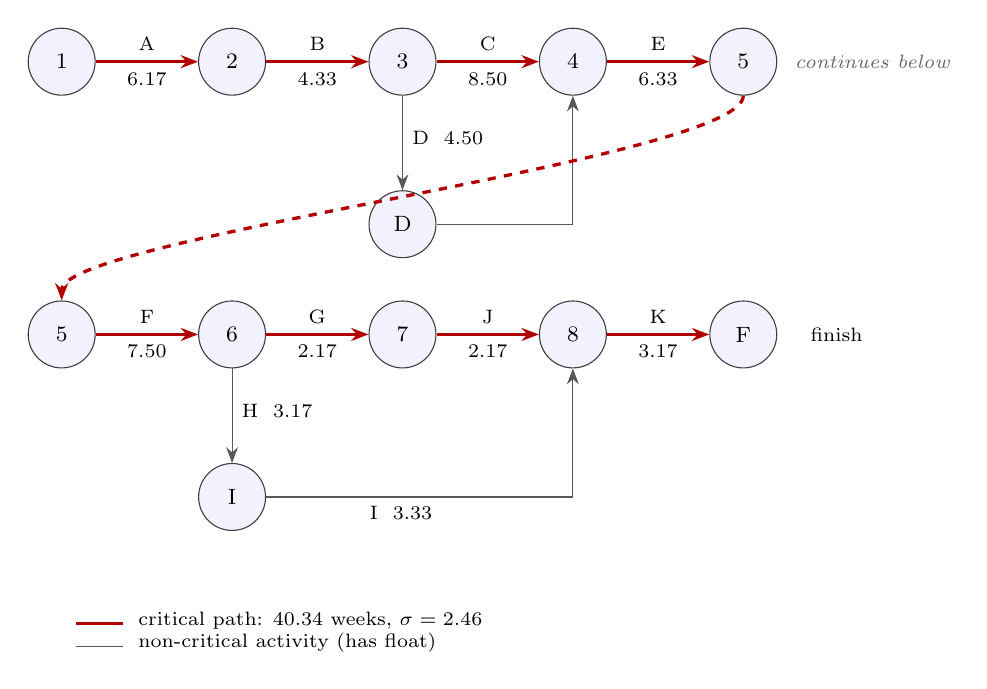
\begin{tikzpicture}[node distance=11mm and 13mm]
  \tikzset{ev/.style={circle, draw=black!75, fill=blue!5, minimum size=8.5mm,
                      font=\footnotesize, inner sep=0pt},
            crit/.style={-{Stealth[length=2.2mm]}, draw=red!70!black, very thick,
                         font=\scriptsize},
            norm/.style={-{Stealth[length=2mm]}, draw=black!65, font=\scriptsize}}
  % --- row 1: events 1..5 -------------------------------------------------
  \node[ev] (n1) {1};
  \node[ev, right=of n1] (n2) {2};
  \node[ev, right=of n2] (n3) {3};
  \node[ev, right=of n3] (n4) {4};
  \node[ev, right=of n4] (n5) {5};
  \node[ev, below=12mm of n3] (nd) {D};
  \draw[crit] (n1) -- node[above]{A} node[below]{6.17} (n2);
  \draw[crit] (n2) -- node[above]{B} node[below]{4.33} (n3);
  \draw[crit] (n3) -- node[above]{C} node[below]{8.50} (n4);
  \draw[crit] (n4) -- node[above]{E} node[below]{6.33} (n5);
  \draw[norm] (n3) -- node[right, pos=0.45]{D \ 4.50} (nd);
  \draw[norm] (nd) -| (n4);

  % --- row 2: events 5..8 and the finish ----------------------------------
  \node[ev, below=26mm of n1] (m5) {5};
  \node[ev, right=of m5] (m6) {6};
  \node[ev, right=of m6] (m7) {7};
  \node[ev, right=of m7] (m8) {8};
  \node[ev, right=of m8] (mf) {F};
  \node[ev, below=12mm of m6] (ni) {I};
  \draw[crit] (m5) -- node[above]{F} node[below]{7.50} (m6);
  \draw[crit] (m6) -- node[above]{G} node[below]{2.17} (m7);
  \draw[crit] (m7) -- node[above]{J} node[below]{2.17} (m8);
  \draw[crit] (m8) -- node[above]{K} node[below]{3.17} (mf);
  \draw[norm] (m6) -- node[right, pos=0.45]{H \ 3.17} (ni);
  \draw[norm] (ni) -| node[pos=0.22, below, font=\scriptsize]{I \ 3.33} (m8);
  \node[right=3mm of mf, font=\scriptsize] {finish};

  % row-continuation marker
  \draw[crit, dashed] (n5.south) .. controls +(0,-8mm) and +(0,8mm) .. (m5.north);
  \node[font=\scriptsize\itshape, black!60, right=1mm of n5] {continues below};

  \node[font=\scriptsize, align=left, below=9mm of ni, xshift=6mm]
       {\textcolor{red!70!black}{\rule{6mm}{1.2pt}} \ critical path: 40.34 weeks, $\sigma = 2.46$\\
        \textcolor{black!65}{\rule{6mm}{0.6pt}} \ non-critical activity (has float)};
\end{tikzpicture}}
\caption{PERT network for Phase 1 with the critical path highlighted}
\label{fig:pert}
\end{figure}

\subsection{Risk Management}
\label{subsec:risk}

Table~\ref{tab:risk} records the risks identified at planning time, together
with the mitigation applied and (where the risk materialised) what
actually happened. Five of the nine anticipated risks occurred.

\begin{longtable}{@{}L{1.0cm} L{3.3cm} C{1.6cm} C{1.6cm} L{5.6cm}@{}}
\caption{Risk register with outcomes}
\label{tab:risk}\\
\toprule
\rowcolor{headblue}
\textbf{ID} & \textbf{Risk} & \textbf{Prob.} & \textbf{Impact} & \textbf{Mitigation and outcome} \\
\midrule
\endfirsthead
\toprule
\rowcolor{headblue}
\textbf{ID} & \textbf{Risk} & \textbf{Prob.} & \textbf{Impact} & \textbf{Mitigation and outcome} \\
\midrule
\endhead
\bottomrule
\endlastfoot

R1 & Gated access to the teacher checkpoints and the BPCC corpus & High & High & Fall back to ungated rotary checkpoints and the Samanantar corpus. \textbf{Occurred.} Mitigation applied; the cost is a lower quality ceiling, reported explicitly \\
\rowcolor{rowgrey}
R2 & No GPU available locally & High & High & Use a cloud GPU (Kaggle, Colab) and later a dedicated A40 VM. \textbf{Occurred.} All final training ran on the A40 VM \\
R3 & Student fails to reach the quality target & Medium & High & Treat data volume, teacher strength and student width as independent levers; report shortfall honestly. \textbf{Partially occurred:} 14 of 22 directions pass \\
\rowcolor{rowgrey}
R4 & Training instability or divergence & Medium & High & Gradient clipping, learning-rate warmup, label smoothing; monitor training loss as a collapse indicator. \textbf{Occurred twice}; both recovered (Section~\ref{sec:collapse}) \\
R5 & Cloud session time limits kill long runs & High & Medium & Resumable runners with per-stage completion markers; persist artifacts outside the session. \textbf{Occurred} on Kaggle's 12-hour cap; resumability absorbed it \\
\rowcolor{rowgrey}
R6 & Quantised model exceeds the size budget & Low & High & Progressive INT8 then INT4 with per-stage measurement. \textbf{Did not occur:} 103.9\,MB against a 200\,MB budget \\
R7 & Inference too slow on CPU & Medium & High & ONNX Runtime with greedy decoding at deployment; beam search only offline. \textbf{Did not occur:} mean 105--202\,ms \\
\rowcolor{rowgrey}
R8 & Dependency and environment conflicts & Medium & Medium & Pin versions; audit the environment before each run. \textbf{Occurred} four times on the VM (Section~\ref{subsec:sw}); each fix folded into the runner \\
R9 & Insufficient corpus for low-resource languages & High & Medium & Prioritise languages with ungated data; document the blocked ones. \textbf{Occurred:} 11 of 22 languages delivered \\

\end{longtable}

\subsection{Team Organisation and Responsibilities}
\label{subsec:team}

The team of four divided the work by pipeline stage, with every member
responsible for the tests covering their own modules. Integration was
continuous: a milestone was not considered closed until the full test suite
passed, which forced interfaces to be agreed early rather than reconciled late.

\begin{table}[H]
\centering
\caption{Division of responsibility}
\label{tab:team}
\begin{tabular}{@{}L{3.3cm} L{2.4cm} J{8.2cm}@{}}
\toprule
\rowcolor{headblue}
\textbf{Member} & \textbf{USN} & \textbf{Primary responsibility} \\
\midrule
Jannat Zafrin & 1BI23AI017 & Literature survey; corpus pipeline (loading, normalisation, filtering, deduplication); evaluation harness and scorecard generation \\
\rowcolor{rowgrey}
Prabhav Sharma & 1BI23AI040 & Teacher integration and the abstraction wall; preference generation ($k$-NN retrieval, chrF ranking, validation); DPO trainer \\
Rishabh Sharma & 1BI23AI047 & \seqkd{} distiller and student trainer; GPU training campaign and runners; quantisation and ONNX export; collapse diagnosis and recovery \\
\rowcolor{rowgrey}
Sindhuja Tiwari & 1BI23AI054 & Inference engine and pivot router; REST API; Next.js client and offline PWA; CLI; test suite and documentation \\
\bottomrule
\end{tabular}
\end{table}

All four members contributed to system design, to the analysis of experimental
results, and to this report. Weekly review meetings with the guide governed
milestone closure, and the project log maintained in the repository records a
dated entry for every working session, which is the source from which
Chapter~\ref{ch:results} is reconstructed.

% ============================== CHAPTER 5 ===================================
\chapter{System Design}
\label{ch:design}

System design bridges the requirements of Chapter~\ref{ch:requirements} and the
implementation of Chapter~\ref{ch:implementation}. It answers the question
\emph{how}: how the system is structured, how it decomposes into modules, what
crosses the boundaries between them, how data is represented, and what the core
algorithms are.

One structural decision dominates the design and is worth stating before the
detail. \setu{} is not a single program but two programs that share a data
format. The training program is large, depends on PyTorch and Transformers, runs
on a GPU, and executes once per direction. The inference program is small,
depends only on ONNX Runtime and SentencePiece, runs on a CPU, and executes
millions of times. They meet at exactly one point: a directory containing a
quantised ONNX model and a SentencePiece tokenizer. Everything else in the
design follows from keeping that boundary clean, because it is what makes the
deployed artifact small enough and offline enough to satisfy the requirements.

\section{System Architecture}
\label{sec:architecture}

Figure~\ref{fig:sysarch} gives the high-level architecture. Data flows left to
right through four stages (corpus, distillation, training, deployment) and
then fans out to the four client interfaces.

% Aspect ratio 4.88: sideways page so the pipeline labels stay legible.
\widefigure{width=\linewidth, keepaspectratio}{figures/system_design.png}%
  {System architecture: \seqkd{} distillation and offline deployment pipeline}{fig:sysarch}

The architecture has four layers.

\textbf{The data layer} ingests parallel corpora, normalises and filters them,
and stores two corpora per direction: the \emph{processed} corpus, which retains
human references and is used only for evaluation, and the \emph{distilled}
corpus, whose targets are the teacher's one-best translations and which is used
for training. Keeping both is what allows evaluation to remain on real
references regardless of what the student was trained on, the property that
makes the comparison in Section~\ref{sec:headtohead} fair.

\textbf{The model layer} holds the teacher behind an abstract interface and the
student behind a trainer. The teacher is used only offline, and only through
three methods. The student is a Marian encoder--decoder trained from scratch.

\textbf{The deployment layer} converts a trained student into a device artifact:
ONNX export, runtime validation, progressive INT8 and INT4 quantisation, and a
per-stage benchmark. Its output is a self-contained directory.

\textbf{The serving layer} loads those directories on demand, caches one engine
per direction, routes each request to a direct model or through the English
pivot, and presents the result through four interfaces that share the routing
code exactly.

\subsection{Design Principles}
\label{subsec:principles}

Five principles were applied consistently and explain most of the specific
choices that follow.

\textbf{One direction, one model.} Each translation direction gets its own
student. This avoids the cross-lingual interference that multilingual
distillation frameworks report \cite{ref:aiokd}, permits an independent quality
gate per direction, and means a collapsed direction can be retrained without
disturbing any other. The cost is storage, 104\,MB per direction, which the
English pivot then bounds at $2n$ rather than $n^2$.

\textbf{The teacher lives behind a wall.} \texttt{IndicTrans2Teacher} is the only
module permitted to import \texttt{transformers}, \texttt{torch} or
\texttt{IndicTransToolkit}. A unit test walks the source tree and fails the
build on any violation. This is what guarantees that the inference path carries
no training dependencies.

\textbf{Configuration, not code.} The language pair, model dimensions,
hyperparameters, corpus sources and cleaning thresholds all live in YAML.
Adding a language is a configuration change and a data fetch. A dedicated test
verifies that the pipeline is pair-agnostic by running it on a different pair
end to end.

\textbf{Fail loudly, never silently.} When no model exists for a requested pair
the engine returns the input unchanged but sets \texttt{stub: true}, so a caller
can never mistake a passthrough for a translation. When the scorecard has no
evidence for a target it prints \textsc{unverified} rather than a pass. This
principle is why the 0.796 ratio in an early report was printed as a failure
rather than rounded up.

\textbf{Resumability by construction.} Every pipeline stage writes a completion
marker. A multi-hour run interrupted by a disconnection resumes at the stage it
reached, which matters because teacher distillation over 500{,}000 sentences is
too expensive to repeat.

\section{Component Design / Module Decomposition}
\label{sec:modules}

The system decomposes into eight modules. Each has a single responsibility, a
defined input and output, and its own tests.

\subsection{Module 1: Corpus Loader}
\label{subsec:mod1}

\textbf{Responsibility:} turn a raw parallel corpus into a clean, deduplicated
set of \texttt{CorpusEntry} objects.

The module streams Samanantar from Hugging Face (streaming rather than
downloading, because the full corpus is tens of gigabytes and only a slice is
needed) and passes each pair through four stages. \emph{Normalisation}
applies Unicode NFC and strips control characters while explicitly preserving
zero-width joiners and non-joiners, which carry meaning in Indic scripts.
\emph{Filtering} removes pairs shorter than 3 or longer than 1024 characters,
pairs whose source-to-target length ratio exceeds 3.0 (a reliable signal of
misalignment in mined data), and pairs in which fewer than half the letters
belong to the expected script. \emph{Deduplication} removes exact duplicates.
\emph{Reporting} records how many pairs each filter removed.

A representative run illustrates the module's value: 50{,}000 input pairs
yielded 49{,}520 clean pairs, with 253 removed for length ratio, 213 for wrong
script, 10 for excessive length and 4 as duplicates. Roughly one pair in a
hundred of web-mined data is unusable, and the wrong-script filter in particular
catches pairs where one side is simply not in the language it claims to be.

\subsection{Module 2: Teacher Distiller}
\label{subsec:mod2}

\textbf{Responsibility:} replace every human reference target with the teacher's
own one-best translation of the source.

\texttt{SeqKDDistiller} batches source sentences, calls the teacher's
\texttt{generate\_candidates\_batch} with $n=1$, and emits new
\texttt{CorpusEntry} objects tagged \texttt{seqkd}. Greedy decoding is used
rather than beam search: it is four to five times faster, which is what makes
distilling half a million sentences feasible within a session, and the resulting
targets are of equivalent utility for training.

The module degrades safely. If the teacher returns an empty candidate for some
sentence, the original human reference is retained for that pair and the event
is counted in the module's statistics, so a teacher hiccup cannot silently
introduce blank training targets.

\subsection{Module 3: \seqkd{} Trainer}
\label{subsec:mod3}

\textbf{Responsibility:} train a 52.6-million-parameter student from scratch on
the distilled corpus.

The trainer implements token-level cross-entropy with five components, each
added in response to an observed failure rather than adopted by convention:

\begin{itemize}
  \item \textbf{PAD masking.} Label positions corresponding to padding are set
        to $-100$ so that the loss ignores them. Before this fix the model
        received free credit for predicting padding, which produced a
        fake-low loss of 0.274 and a decoder that ignored the source entirely.
  \item \textbf{Linear warmup and decay.} The warmup length is capped at
        10\,\% of the run. A from-scratch Transformer trained at a constant
        learning rate underfits badly; the configuration option existed but was
        being silently ignored.
  \item \textbf{Label smoothing (0.1) and dropout (0.2).} Standard regularisers
        against overconfidence and memorisation.
  \item \textbf{Gradient-norm clipping at 1.0.} The single most important
        stabiliser. Without it, a 200{,}000-sentence run collapsed to a constant
        output while the identical code at 120{,}000 sentences had succeeded: more steps simply meant more opportunities to hit a gradient spike.
  \item \textbf{Generation safeguards.} Decoding suppresses the PAD, UNK and BOS
        tokens and forbids repeated 3-grams, so output can never be empty and
        cannot degenerate into a repeated phrase.
\end{itemize}

The module also implements DPO with a frozen supervised-fine-tuning reference
model. A test enforces that the reference model's parameters never receive
gradients, since an unfrozen reference silently reduces DPO to a no-op. This
path is retained for the reported comparison but is not used for the shipped
models.

\subsection{Module 4: Quantiser}
\label{subsec:mod4}

\textbf{Responsibility:} convert a trained PyTorch checkpoint into a deployable
ONNX artifact.

The module exports to FP32 ONNX, validates the export by running it through ONNX
Runtime and comparing outputs, then quantises progressively (INT8 first, INT4
second), benchmarking size and latency at each stage. The measured progression
for a 52.6-million-parameter student is 410.9\,MB FP32, 104.6\,MB INT8 and
103.9\,MB INT4.

The near-identity of the INT8 and INT4 sizes is an honest limitation rather than
a measurement error: the ONNX Runtime CPU execution provider has no true 4-bit
kernel, so INT4 export falls back to 8-bit storage for most tensors. The INT4
variant is nonetheless the one shipped, because it benchmarked marginally faster
and, in several directions, marginally more accurate.

\subsection{Module 5: Inference Engine and Pivot Router}
\label{subsec:mod5}

\textbf{Responsibility:} translate text using a quantised student, offline, and
route requests to the right student.

\texttt{InferenceEngine} loads an ONNX session and a local SentencePiece
tokenizer, encodes the source, decodes greedily, and returns a
\texttt{TranslationResult} carrying the translated text and the measured
latency. An \texttt{assert\_offline()} helper disables all sockets to prove that
inference needs no network.

The router sits above it and solves the coverage problem. Given a source and
target language it resolves both to FLORES codes, rejects identical pairs and
unknown codes, then checks for a directly trained model. If one exists it
translates in a single hop. If not (the case for every Indic-to-Indic pair,
since no ungated Indic-to-Indic teacher was available), it checks whether both
source\arrowto{}English and English\arrowto{}target models exist, and if so
chains them, returning the combined latency and a \texttt{pivot: "en"} flag. The
arithmetic is favourable: 22 direct models serve 132 usable directions, and
measured two-hop latency is approximately 50--65\,ms.

Engines are cached one per pair, so a direction is loaded from disk at most
once, and every interface calls this single router rather than reimplementing
routing. Consolidating the routing logic here fixed a real defect: the CLI had
previously constructed an engine with the default configured pair, so
\texttt{-{}-src as} silently translated using the Hindi model.

\subsection{Module 6: REST API}
\label{subsec:mod6}

\textbf{Responsibility:} expose the engine over HTTP.

A FastAPI service provides four endpoints. \texttt{POST /translate} accepts a
source language, target language and text and returns the translation with
latency and pivot information. \texttt{GET /languages} returns the registry of
22 scheduled languages plus English, marking which are trained. \texttt{GET
/models} scans the models directory and reports every discovered pair with its
quantisation variant and size on disk. \texttt{GET /health} reports readiness.
CORS is enabled so that a browser client can call the service directly.

\subsection{Module 7: Client Interfaces}
\label{subsec:mod7}

\textbf{Responsibility:} make the engine usable.

Four clients share the engine. The \textbf{CLI} accepts text from an argument, a
file or standard input and emits plain text or JSON. The \textbf{Next.js web
client} provides a translator console with source and target pickers, a swap
control, live latency display and an on-device indicator; all 23 languages
appear in the picker, with the trained ones grouped as available and the
remainder shown but disabled, so coverage is visible rather than hidden. The
\textbf{offline progressive web application} caches its shell through a service
worker and continues to function without a network. \textbf{Mobile SDK stubs}
for Android and iOS wrap the same API surface.

\subsection{Module 8: Evaluator and Expansion Mechanisms}
\label{subsec:mod8}

\textbf{Responsibility:} measure quality, and provide a route to adding
languages.

The evaluator computes BLEU and chrF with sacreBLEU on a held-out slice of real
human references, computes the teacher's score on the identical slice, and
reports the ratio. Loaders for FLORES-200 and IN22 are implemented for
benchmark-grade numbers, along with COMET scoring and paired-bootstrap
significance testing.

Two expansion mechanisms are implemented and tested. \textbf{All-in-One
knowledge distillation} trains one student across several directions with
temperature-sampled cross-lingual balancing and a coverage report; a sampling
temperature above 1.0 flattens the distribution towards uniform and so protects
low-resource directions from being swamped. \textbf{Elastic Weight
Consolidation} adds a diagonal-Fisher penalty that anchors parameters important
to previously learned languages, enabling a new language to be added without a
full retrain. Its tests prove the penalty is zero at the snapshot point, grows
with distance from it, and (measured rather than assumed) keeps
Fisher-weighted drift on an old task below that of plain fine-tuning after a
conflicting new task.

\needspace{14\baselineskip}
\section{Interface Design}
\label{sec:interface}

\subsection{External Interfaces}
\label{subsec:extinterface}

\begin{longtable}{@{}L{2.5cm} L{4.2cm} J{7.4cm}@{}}
\caption{External interface specification}
\label{tab:interfaces}\\
\toprule
\rowcolor{headblue}
\textbf{Component} & \textbf{Description} & \textbf{Details and example} \\
\midrule
\endfirsthead
\toprule
\rowcolor{headblue}
\textbf{Component} & \textbf{Description} & \textbf{Details and example} \\
\midrule
\endhead
\bottomrule
\endlastfoot

REST: translate & Primary translation endpoint & \texttt{POST /translate} with body \texttt{\{source\_lang, target\_lang, text\}}; returns \texttt{\{translated\_text, latency\_ms, pivot, stub\}}. Example request: \texttt{\{"source\_lang":"hi", "target\_lang":"en", "text":"..."\}} \\
\rowcolor{rowgrey}
REST: languages & Language registry & \texttt{GET /languages} $\rightarrow$ 22 scheduled languages plus English, each with ISO code, FLORES code, script and endonym \\
REST: models & Model discovery & \texttt{GET /models} $\rightarrow$ \texttt{\{"count": 22, "models": [\{pair, variant, size\_mb\}, ...]\}} \\
\rowcolor{rowgrey}
REST: health & Readiness probe & \texttt{GET /health} $\rightarrow$ \texttt{\{"status":"ok", "stub": false\}} \\
CLI & Command-line translation & \texttt{python setu\_cli.py -{}-src hi -{}-tgt en -{}-text "..."}; also \texttt{-{}-file} and standard input, with \texttt{-{}-json} output \\
\rowcolor{rowgrey}
Web client & Browser translator console & Language pickers grouped into available and not-yet-trained, swap control, live latency, on-device badge, curated Indic-to-Indic examples \\
Offline PWA & Installable offline client & Service-worker shell caching; functions with no network after first load \\
\rowcolor{rowgrey}
Mobile SDK & Android and iOS wrapper & \texttt{translate(text, srcLang, tgtLang)} over the same engine \\
Training CLI & Pipeline entry points & \texttt{setu-data}, \texttt{setu-distill}, \texttt{setu-quantize}, \texttt{setu-eval}, \texttt{setu-report}, and \texttt{scripts/train\_full.py} \\

\end{longtable}

\subsection{User Interface Design}
\label{subsec:uidesign}

The web client was designed around one principle: a user must be able to tell,
at a glance, whether a translation was produced on their device and how good the
coverage is for their language. Three affordances implement it.

The \textbf{on-device badge} reports whether the response came from a real
quantised model or the passthrough stub, alongside the measured latency in
milliseconds. A user is never shown a number without knowing what produced it.

The \textbf{language picker} lists all 23 languages, not only the trained ones.
Trained languages are grouped under an ``available now'' heading; the remaining
eleven appear below, visibly disabled and labelled as Phase 2. Hiding untrained
languages would have made the system look complete; showing them disabled makes
the actual coverage legible.

The \textbf{pivot indicator} tells the user when a translation was routed
through English, because a two-hop translation has different failure
characteristics from a single-hop one and the user is entitled to know.

Visually the client uses a warm paper-and-ink palette with a single accent
colour, a light and dark theme, and typography that names every language in its
own script (\dev{हिन्दी}, \ben{বাংলা}, \tam{தமிழ்}, \tel{తెలుగు},
\kan{ಕನ್ನಡ}, \mal{മലയാളം}, \guj{ગુજરાતી}, \ory{ଓଡ଼ିଆ}, \gur{ਪੰਜਾਬੀ}) rather
than transliterating them into Latin. Fonts are self-hosted so that the client
loads no external resource at run time, which is a functional requirement rather
than a stylistic one.

\section{Data Structure Design}
\label{sec:datastructures}

Four data objects carry all information between modules. Their field names are
stable across the entire codebase, which is what allows modules to be developed
and tested independently.

\begin{table}[H]
\centering
\caption{Core data structures}
\label{tab:datastructures}
\begin{tabular}{@{}L{4.0cm} L{4.1cm} J{6.0cm}@{}}
\toprule
\rowcolor{headblue}
\textbf{Structure} & \textbf{Fields} & \textbf{Purpose} \\
\midrule
\texttt{CorpusEntry} & \texttt{src\_lang}, \texttt{tgt\_lang}, \texttt{src\_text}, \texttt{tgt\_text}, \texttt{source} & One parallel sentence pair. The \texttt{source} tag distinguishes a human reference from a \texttt{seqkd} teacher target, so the two corpora never mix \\
\rowcolor{rowgrey}
\texttt{PreferencePair} & \texttt{src\_text}, \texttt{preferred\_tgt}, \texttt{dispreferred\_tgt}, \texttt{quality\_delta} & One DPO training example. \texttt{quality\_delta} is the chrF gap; pairs below a threshold are discarded as too noisy to teach from \\
\texttt{ModelConfig} & \texttt{language\_pair}, \texttt{params}, \texttt{quantization} & Full student specification: architecture, layer counts, hidden size, vocabulary size, sequence length, quantisation mode \\
\rowcolor{rowgrey}
\texttt{TranslationResult} & \texttt{translated\_text}, \texttt{src\_lang}, \texttt{tgt\_lang}, \texttt{latency\_ms}, \texttt{pivot} & One translation with its provenance. \texttt{pivot} is \texttt{None} for direct translation and \texttt{"en"} for a chained one \\
\bottomrule
\end{tabular}
\end{table}

\subsection{On-Disk Layout}
\label{subsec:ondisk}

Corpora are stored as JSONL, one entry per line, which streams without loading
the whole file and appends cheaply. Reports are JSON. A deployed model
directory is self-contained:

\begin{verbatim}
models/<src_flores>-<tgt_flores>/
  |-- int4/       encoder + decoder ONNX (103.9 MB, shipped)
  |-- int8/       the INT8 variant (104.6 MB)
  |-- onnx/       the FP32 export (410.9 MB, not shipped)
  |-- tokenizer/  SentencePiece model and vocabulary
  `-- quantize_report.json    per-stage size and latency
\end{verbatim}

Model discovery scans for exactly this layout, which is why dropping a trained
model directory into place is all that is needed for the API to serve it.

\subsection{The Tokenizer's Reserved Tags}
\label{subsec:tokenizer}

The SentencePiece vocabulary is 16{,}000 unigram tokens, chosen after a
32{,}000-token vocabulary was measured to leave most tokens undertrained on the
available data and to produce degenerate decoding. All 23 FLORES language tags
are reserved as special tokens from the very first training run, even for
languages not yet trained. This costs 23 vocabulary slots and buys a guarantee:
token identifiers do not shift when a language is added, so previously trained
models remain valid and no re-tokenisation is ever required.

\section{Algorithm Design}
\label{sec:algorithms}

\subsection{Algorithm 1: Sequence-Level Knowledge Distillation}
\label{subsec:alg1}

This is the core training algorithm and the one the empirical comparison
selected.

\begin{longtable}{@{}L{14.0cm}@{}}
\caption{Algorithm 1: \seqkd{} training of one direction}
\label{tab:alg1}\\
\toprule
\rowcolor{headblue}
\textbf{Input:} cleaned corpus $C = \{(x_i, y_i)\}_{i=1}^{N}$; teacher $T$; student architecture $\theta$ \\
\rowcolor{headblue}
\textbf{Output:} trained student parameters $\theta^{*}$ \\
\midrule
\endfirsthead
\multicolumn{1}{c}{\textit{Table \thetable{} (continued)}}\\
\toprule
\rowcolor{headblue}
\textbf{Input:} cleaned corpus $C = \{(x_i, y_i)\}_{i=1}^{N}$; teacher $T$; student architecture $\theta$ \\
\rowcolor{headblue}
\textbf{Output:} trained student parameters $\theta^{*}$ \\
\midrule
\endhead
\midrule
\multicolumn{1}{r}{\textit{continued on next page}}\\
\endfoot
\bottomrule
\endlastfoot

\textbf{1.} \textbf{for} each batch $B \subseteq C$ \textbf{do} \\
\textbf{2.} \quad $\hat{y}_i \leftarrow T.\textsc{decode}(x_i)$ \quad \textit{// greedy one-best; discard the human $y_i$} \\
\textbf{3.} \quad \textbf{if} $\hat{y}_i$ is empty \textbf{then} $\hat{y}_i \leftarrow y_i$ \quad \textit{// safe fallback, counted} \\
\textbf{4.} \quad append $(x_i, \hat{y}_i)$ to the distilled corpus $D$ \\
\textbf{5.} \textbf{end for} \\
\textbf{6.} initialise $\theta$ randomly; initialise AdamW with linear warmup then decay \\
\textbf{7.} \textbf{for} epoch $= 1 \ldots E$ \textbf{do} \\
\textbf{8.} \quad \textbf{for} each batch $(x, \hat{y}) \subseteq D$ \textbf{do} \\
\textbf{9.} \quad\quad $\ell \leftarrow \textsc{CrossEntropy}(\theta(x), \hat{y})$ with pad labels set to $-100$ and label smoothing $0.1$ \\
\textbf{10.} \quad\quad backpropagate; $\textsc{ClipGradNorm}(\theta, 1.0)$; optimiser step; scheduler step \\
\textbf{11.} \quad \textbf{end for} \\
\textbf{12.} \quad evaluate on held-out \emph{human} references; record BLEU, chrF and the teacher ratio \\
\textbf{13.} \textbf{end for} \\
\textbf{14.} \textbf{return} $\theta^{*}$ \\
\end{longtable}

Three details carry the algorithm's correctness. Line~2 discards the human
target; that is the whole method, and it is what breaks the reference-noise
ceiling. Line~9's $-100$ masking is what keeps the loss honest. Line~12
evaluates on human references even though training used teacher targets, which
is what makes the numbers comparable with a reference-trained baseline.

\subsection{Algorithm 2: English-Pivot Routing}
\label{subsec:alg2}

\begin{longtable}{@{}L{14.0cm}@{}}
\caption{Algorithm 2: routing a translation request}
\label{tab:alg2}\\
\toprule
\rowcolor{headblue}
\textbf{Input:} text $t$; source language $s$; target language $g$ \\
\rowcolor{headblue}
\textbf{Output:} translation, pivot flag, stub flag \\
\midrule
\endfirsthead
\multicolumn{1}{c}{\textit{Table \thetable{} (continued)}}\\
\toprule
\rowcolor{headblue}
\textbf{Input:} text $t$; source language $s$; target language $g$ \\
\rowcolor{headblue}
\textbf{Output:} translation, pivot flag, stub flag \\
\midrule
\endhead
\midrule
\multicolumn{1}{r}{\textit{continued on next page}}\\
\endfoot
\bottomrule
\endlastfoot

\textbf{1.} $s \leftarrow \textsc{ResolveFlores}(s)$; \ $g \leftarrow \textsc{ResolveFlores}(g)$ \quad \textit{// raises on an unknown code} \\
\textbf{2.} \textbf{if} $s = g$ \textbf{then raise} \textsc{ValueError} \quad \textit{// identical source and target} \\
\textbf{3.} $d \leftarrow$ \texttt{"}$s$\texttt{-}$g$\texttt{"} \\
\textbf{4.} \textbf{if} \textsc{ModelExists}($d$) \textbf{then return} $(\textsc{Engine}(d).\textsc{translate}(t),\ \textsc{None},\ \textsc{False})$ \\
\textbf{5.} \textbf{if} $s \neq$ \texttt{eng\_Latn} \textbf{and} $g \neq$ \texttt{eng\_Latn} \textbf{then} \\
\textbf{6.} \quad $h_1 \leftarrow$ \texttt{"}$s$\texttt{-eng\_Latn"}; \ $h_2 \leftarrow$ \texttt{"eng\_Latn-}$g$\texttt{"} \\
\textbf{7.} \quad \textbf{if} \textsc{ModelExists}($h_1$) \textbf{and} \textsc{ModelExists}($h_2$) \textbf{then} \\
\textbf{8.} \quad\quad $r_1 \leftarrow \textsc{Engine}(h_1).\textsc{translate}(t)$ \quad \textit{// source to English} \\
\textbf{9.} \quad\quad $r_2 \leftarrow \textsc{Engine}(h_2).\textsc{translate}(r_1.\text{text})$ \quad \textit{// English to target} \\
\textbf{10.} \quad\quad \textbf{return} $(r_2 \text{ with latency } r_1.\text{ms} + r_2.\text{ms},\ \texttt{"en"},\ \textsc{False})$ \\
\textbf{11.} \quad \textbf{end if} \\
\textbf{12.} \textbf{end if} \\
\textbf{13.} \textbf{return} $(t,\ \textsc{None},\ \textsc{True})$ \quad \textit{// passthrough, explicitly flagged as a stub} \\
\end{longtable}

Engines are memoised per pair, so the model-existence checks on lines 4 and 7
are cheap after the first call. Line~13 is the honesty guarantee: when nothing
can translate the request the input is returned unchanged and explicitly marked,
never presented as a translation.

\subsection{Algorithm 3: Progressive Quantisation}
\label{subsec:alg3}

\begin{table}[H]
\centering
\caption{Algorithm 3: export and progressive quantisation}
\label{tab:alg3}
\begin{tabular}{@{}L{14.0cm}@{}}
\toprule
\rowcolor{headblue}
\textbf{Input:} trained checkpoint $\theta^{*}$; benchmark sentence set $S$ \\
\rowcolor{headblue}
\textbf{Output:} INT8 and INT4 ONNX artifacts with a size and latency report \\
\midrule
\textbf{1.} export $\theta^{*}$ to FP32 ONNX; \textbf{assert} the checkpoint path exists (fail clearly, not as a remote identifier) \\
\textbf{2.} validate: run the ONNX graph through ONNX Runtime and compare against the PyTorch output \\
\textbf{3.} $m_{32} \leftarrow \textsc{SizeMB}$; \ $(p_{50}, p_{90}, p_{\max}) \leftarrow \textsc{Benchmark}(S)$ \\
\textbf{4.} apply dynamic INT8 quantisation; re-measure size and latency \\
\textbf{5.} apply INT4 quantisation; re-measure size and latency \\
\textbf{6.} \textbf{for} each variant \textbf{do assert} $\text{size} \leq 200$\,MB \textbf{and} $p_{90} < 500$\,ms \\
\textbf{7.} verify translation succeeds with all network sockets disabled \\
\textbf{8.} write \texttt{quantize\_report.json}; package the chosen variant with its tokenizer \\
\bottomrule
\end{tabular}
\end{table}

\subsection{Algorithm 4: Preference Pair Generation (Reported Baseline)}
\label{subsec:alg4}

This algorithm produced the DPO training data for the comparison in
Section~\ref{sec:headtohead}. It is retained in the system and documented here
because the negative result it supports is one of the project's findings, but it
is not used for the shipped models.

\begin{table}[H]
\centering
\caption{Algorithm 4: chrF-ranked preference pair construction}
\label{tab:alg4}
\begin{tabular}{@{}L{14.0cm}@{}}
\toprule
\rowcolor{headblue}
\textbf{Input:} corpus entries; teacher $T$; candidate count $n$; neighbour count $k$; minimum delta $\delta$ \\
\rowcolor{headblue}
\textbf{Output:} validated \texttt{PreferencePair} list \\
\midrule
\textbf{1.} \textbf{for} each entry $(x, y)$ \textbf{do} \\
\textbf{2.} \quad $A \leftarrow T.\textsc{generateCandidates}(x, n)$ \quad \textit{// beam search, $n$ returned sequences} \\
\textbf{3.} \quad $A \leftarrow A \cup \textsc{KnnNeighbourTranslations}(x, k)$ \quad \textit{// char n-gram TF-IDF retrieval} \\
\textbf{4.} \quad score every $a \in A$ by sentence chrF against the human reference $y$ \\
\textbf{5.} \quad $a^{+} \leftarrow \arg\max_a \textsc{chrF}(a, y)$ \\
\textbf{6.} \quad \textbf{for} each $a^{-} \in A \setminus \{a^{+}\}$ \textbf{do} \\
\textbf{7.} \quad\quad $\Delta \leftarrow \textsc{chrF}(a^{+}, y) - \textsc{chrF}(a^{-}, y)$ \\
\textbf{8.} \quad\quad \textbf{if} $\Delta \geq \delta$ \textbf{then} emit $(x, a^{+}, a^{-}, \Delta)$ \quad \textit{// otherwise too noisy to teach from} \\
\textbf{9.} \quad \textbf{end for} \\
\textbf{10.} \textbf{end for} \\
\textbf{11.} \textbf{assert} $\textsc{chrF}(a^{+}) > \textsc{chrF}(a^{-})$ for every emitted pair \quad \textit{// validation gate} \\
\bottomrule
\end{tabular}
\end{table}

A representative run turned 500 corpus entries into 3{,}494 candidates and
2{,}074 validated pairs, discarding 920 for insufficient quality delta; the
delta distribution had a median of 31.3 chrF points. On GPU the same pipeline
produced 33{,}535 validated pairs from 8{,}000 entries. The preference data is
therefore plentiful and well separated, which is precisely why the negative
result is informative. DPO trained on this data reaches a margin accuracy of
1.0, ranking every preferred candidate above its dispreferred counterpart, and
still does not improve translation quality over sequence-level distillation.

% ============================== CHAPTER 6 ===================================
\chapter{Implementation}
\label{ch:implementation}

This chapter describes how the design of Chapter~\ref{ch:design} was realised in
code. It covers the implementation strategy and the standards applied, presents
the significant source with commentary, and discusses the optimisations that
made the system fit the memory, latency and size budgets. Complete source is not
reproduced (the repository contains roughly six thousand lines), but every
component whose behaviour is non-obvious is shown and explained.

\section{Implementation Approaches}
\label{sec:implapproach}

\subsection{Development Strategy}
\label{subsec:strategy}

The project was implemented as a sequence of vertical slices rather than as
horizontal layers. Milestone M0 delivered a complete, working, end-to-end
system in which the translation engine was a passthrough stub: the command-line
tool accepted a language pair, loaded configuration, called an engine and
printed output. Nothing translated anything, but every interface between
components existed and was under test. Each subsequent milestone replaced one
stub with a real implementation, and the test suite grew monotonically.

This ordering was chosen deliberately, and it paid for itself. Because the
inference interface was fixed at M0, the ONNX engine that arrived at M5 was a
drop-in replacement; because \texttt{TranslationResult} was defined at M0, the
pivot router added at Phase~2 only needed one new optional field. The
alternative, building the training pipeline first and the interfaces last,
would have deferred every integration problem to the end of the project.

Three standards were applied throughout.

\textbf{Configuration over code.} No language pair, dimension, threshold or
hyperparameter appears as a literal in a module. Everything lives in YAML under
\texttt{configs/}, and a test verifies the pipeline is pair-agnostic by running
it on a pair other than the default.

\textbf{One boundary for the teacher.} The teacher's dependencies may be
imported by exactly one file, enforced by a test that scans the source tree.

\textbf{Test-first for anything subtle.} Mechanisms whose failure is silent were
given tests before implementation. The DPO reference model must stay frozen; the
EWC penalty must be zero at the snapshot and positive away from it; the
scorecard must print \textsc{unverified} rather than a pass when evidence is
absent. Each of these is a property that no amount of manual inspection reliably
catches.

\subsection{Repository Structure}
\label{subsec:repostructure}

\begin{lstlisting}[language=bash, caption={Repository layout}, label={lst:layout}]
SETU/
|-- setu_cli.py              # CLI entry point
|-- configs/                 # languages, model, training, data, teacher, preference
|   |-- model.yaml           #   CPU development student
|   `-- model.gpu.yaml       #   52.6M GPU student
|-- scripts/
|   |-- train_full.py        # teacher ceiling + train + evaluate in one command
|   |-- build_scores.py      # scorecard generation from per-direction reports
|   `-- translation_suite.py # loads each model and checks its output is healthy
|-- src/setu/
|   |-- types.py             # CorpusEntry, PreferencePair, ModelConfig, TranslationResult
|   |-- config.py            # YAML loaders, language registry, ISO <-> FLORES
|   |-- corpus/              # loader, normalize, filters, dedup, pipeline
|   |-- teacher/             # base (the wall) + indictrans2 backend
|   |-- distill/             # SeqKDDistiller + pipeline
|   |-- preference/          # knn, generator, validate, pipeline
|   |-- training/            # tokenizer, student, dataset, sft, dpo, aio_kd, ewc
|   |-- eval/                # metrics, testsets, comet, significance
|   |-- quantize/            # ONNX export + progressive quantisation
|   |-- inference/           # engine, onnx_engine, router
|   `-- report.py            # final scorecard
|-- interfaces/rest/app.py   # FastAPI service
|-- frontend/                # Next.js client and offline PWA
|-- vm/                      # GPU VM runners and training outputs
`-- tests/                   # 85 tests
\end{lstlisting}

\section{Coding Details and Code Efficiency}
\label{sec:coding}

\subsection{The Teacher Abstraction and Its Wall}
\label{subsec:codewall}

Every dependency on IndicTrans2 is confined to one class behind a three-method
interface. The abstraction is narrow on purpose: a distiller needs only to
generate candidates and score them.

\begin{lstlisting}[language=Python, caption={The teacher interface (\texttt{src/setu/teacher/base.py})}, label={lst:teacherbase}]
class TeacherModel:
    """Abstract teacher. Only IndicTrans2Teacher may import transformers/torch."""

    def generate_candidates(self, src_text: str, src_lang: str,
                            tgt_lang: str, n: int = 4) -> list[str]:
        """Return n candidate translations, best first."""
        raise NotImplementedError

    def generate_candidates_batch(self, src_texts: list[str], src_lang: str,
                                  tgt_lang: str, n: int = 4) -> list[list[str]]:
        """Batched form -- the only method the SeqKD distiller needs."""
        raise NotImplementedError

    def score_candidates(self, candidates: list[str],
                         reference: str) -> list[float]:
        """Sentence-level chrF of each candidate against the reference."""
        raise NotImplementedError
\end{lstlisting}

The wall is enforced mechanically. The test below walks the source tree and
fails if any module other than the designated backend imports the teacher's
dependencies. Without it the restriction would erode within weeks, and the
deployed artifact would silently acquire a PyTorch dependency.

\begin{lstlisting}[language=Python, caption={Enforcing the teacher wall (\texttt{tests/test\_teacher.py})}, label={lst:wall}]
FORBIDDEN = ("transformers", "torch", "IndicTransToolkit")
ALLOWED   = {"src/setu/teacher/indictrans2.py"}

def test_teacher_wall():
    """No module outside the backend may import the teacher's dependencies."""
    for path in Path("src/setu").rglob("*.py"):
        rel = path.as_posix()
        if rel in ALLOWED or "/training/" in rel or "/quantize/" in rel:
            continue                      # training and export legitimately use torch
        source = path.read_text()
        for name in FORBIDDEN:
            assert f"import {name}" not in source, f"{rel} imports {name}"
\end{lstlisting}

\subsection{Corpus Cleaning}
\label{subsec:codecorpus}

The cleaning filters encode domain knowledge about Indic text that a generic
text pipeline would get wrong. Two details matter. Zero-width joiners and
non-joiners must survive normalisation, because they distinguish valid
conjuncts; a naive control-character strip corrupts correct text. And the
script-fraction filter is what removes mined pairs in which one side is simply
not in the claimed language.

\begin{lstlisting}[language=Python, caption={Corpus filters (\texttt{src/setu/corpus/filters.py})}, label={lst:filters}]
ZWJ, ZWNJ = "\u200d", "\u200c"   # zero-width joiner / non-joiner

def normalize(text: str) -> str:
    """NFC normalise and strip control characters, preserving ZWJ/ZWNJ."""
    text = unicodedata.normalize("NFC", text)
    return "".join(
        ch for ch in text
        if unicodedata.category(ch) != "Cc" or ch in (ZWJ, ZWNJ, "\n", "\t")
    )

def passes_length_ratio(src: str, tgt: str, max_ratio: float = 3.0) -> bool:
    """Reject misaligned pairs: mined corpora pair unrelated sentences."""
    if not src or not tgt:
        return False
    ratio = max(len(src), len(tgt)) / min(len(src), len(tgt))
    return ratio <= max_ratio

def passes_script_fraction(text: str, script: str, minimum: float = 0.5) -> bool:
    """At least `minimum` of the letters must belong to the expected script."""
    letters = [ch for ch in text if ch.isalpha()]
    if not letters:
        return False
    in_script = sum(1 for ch in letters if script_of(ch) == script)
    return in_script / len(letters) >= minimum
\end{lstlisting}

\subsection{The \seqkd{} Distiller}
\label{subsec:codedistill}

The distiller is short, which is appropriate: sequence-level distillation is a
simple idea, and the project's contribution is the evidence that it is the right
one, not the code that implements it.

\begin{lstlisting}[language=Python, caption={Sequence-level distillation (\texttt{src/setu/distill/distiller.py})}, label={lst:distill}]
class SeqKDDistiller:
    """Replace each entry's human target with the teacher's 1-best translation."""

    def __init__(self, teacher: TeacherModel, batch_size: int = 32):
        self.teacher = teacher
        self.batch_size = batch_size
        self.stats = {"entries": 0, "empty": 0}

    def distill(self, entries: list[CorpusEntry]) -> list[CorpusEntry]:
        out: list[CorpusEntry] = []
        for start in range(0, len(entries), self.batch_size):
            chunk = entries[start:start + self.batch_size]
            cands = self.teacher.generate_candidates_batch(
                [e.src_text for e in chunk],
                chunk[0].src_lang, chunk[0].tgt_lang, n=1,
            )
            for e, c in zip(chunk, cands):
                if c and c[0].strip():
                    tgt = c[0]                  # the teacher's target replaces the human one
                else:
                    tgt = e.tgt_text            # safe fallback, never a blank target
                    self.stats["empty"] += 1
                out.append(CorpusEntry(e.src_lang, e.tgt_lang,
                                       e.src_text, tgt, "seqkd"))
            self.stats["entries"] += len(chunk)
        return out
\end{lstlisting}

The \texttt{source} field is set to \texttt{"seqkd"} so that a distilled corpus
can never be mistaken for a reference corpus downstream. The evaluation code
asserts that it is scoring against entries whose source is \emph{not}
\texttt{seqkd}, which is the mechanical guarantee behind the fairness of
Section~\ref{sec:headtohead}.

\subsection{The Training Loop}
\label{subsec:codetrain}

This is the most-debugged code in the project. Every line commented below
corresponds to a failure that was observed and diagnosed; the run history is in
Section~\ref{sec:runlog}.

\begin{lstlisting}[language=Python, caption={Supervised training step with all four stabilisers (\texttt{src/setu/training/sft.py})}, label={lst:sft}]
def train(self, dataset) -> dict:
    total_steps = len(dataloader) * self.epochs
    # Warmup was previously read from config and silently ignored; a constant LR
    # underfits a from-scratch transformer. Cap warmup at 10% of the run.
    warmup = min(self.config.get("warmup_steps", 0), max(1, total_steps // 10))
    scheduler = get_linear_schedule_with_warmup(self.optimizer, warmup, total_steps)

    for epoch in range(self.epochs):
        for batch in dataloader:
            outputs = self.model(input_ids=batch["input_ids"],
                                 attention_mask=batch["attention_mask"],
                                 labels=batch["labels"])   # labels use -100 at PAD
            if self.label_smoothing > 0:
                loss = F.cross_entropy(
                    outputs.logits.view(-1, outputs.logits.size(-1)),
                    batch["labels"].view(-1),
                    ignore_index=-100,                  # never score padding
                    label_smoothing=self.label_smoothing,
                )
            else:
                loss = outputs.loss
            loss.backward()
            # The single most important stabiliser: without clipping, a 200k-sentence
            # run collapsed to constant output while 120k on the same code succeeded.
            torch.nn.utils.clip_grad_norm_(self.model.parameters(), self.max_grad_norm)
            self.optimizer.step()
            scheduler.step()
            self.optimizer.zero_grad()
\end{lstlisting}

The dataset builds the labels, and the single most consequential line in the
entire training path is the padding mask:

\begin{lstlisting}[language=Python, caption={Label construction (\texttt{src/setu/training/dataset.py})}, label={lst:dataset}]
def encode_target(self, text: str) -> list[int]:
    """Labels are [tokens, EOS] with NO leading BOS: HuggingFace already prepends
    the decoder start token, so adding one wastes a decode step and creates a
    train/generate mismatch that produced empty output in an early run."""
    ids = self.sp.encode(text)[: self.max_seq_len - 1]
    return ids + [self.eos_id]

def collate(self, batch: list[dict]) -> dict:
    labels = pad_sequence([b["labels"] for b in batch], batch_first=True,
                          padding_value=PAD_ID)
    # -100, not PAD: HuggingFace's loss uses ignore_index=-100. Padding with PAD
    # gave the model free credit for predicting PAD, producing a fake-low loss of
    # 0.274 and a decoder that ignored the source entirely.
    labels[labels == PAD_ID] = -100
    return {"input_ids": ..., "attention_mask": ..., "labels": labels}
\end{lstlisting}

\subsection{The Inference Router}
\label{subsec:coderouter}

The router is the whole of \setu{}'s multilingual coverage story. It is also the
one place where routing logic exists, which is what prevents the interfaces from
diverging.

\begin{lstlisting}[language=Python, caption={English-pivot routing (\texttt{src/setu/inference/router.py})}, label={lst:router}]
@lru_cache(maxsize=None)
def engine_for_pair(pair: str) -> InferenceEngine:
    """One cached engine per pair; a pair with no model on disk stays a stub."""
    return InferenceEngine(ModelConfig(language_pair=pair))

def translate(text, src_lang, tgt_lang) -> tuple[TranslationResult, str | None, bool]:
    """Returns (result, pivot, stub). Raises ValueError on unknown or equal codes."""
    src, tgt = resolve_language(src_lang), resolve_language(tgt_lang)
    if src["iso"] == tgt["iso"]:
        raise ValueError(f"Source and target language are both {src['iso']!r}")

    direct = f"{src['flores']}-{tgt['flores']}"
    if _available(direct):
        return engine_for_pair(direct).translate(text, src["iso"], tgt["iso"]), None, False

    # No direct model: chain source -> English -> target if both halves exist.
    eng = load_languages()["en"]["flores"]            # eng_Latn
    if src["iso"] != "en" and tgt["iso"] != "en":
        hop1, hop2 = f"{src['flores']}-{eng}", f"{eng}-{tgt['flores']}"
        if _available(hop1) and _available(hop2):
            r1 = engine_for_pair(hop1).translate(text, src["iso"], "en")
            r2 = engine_for_pair(hop2).translate(r1.translated_text, "en", tgt["iso"])
            return (TranslationResult(
                        translated_text=r2.translated_text,
                        src_lang=src["iso"], tgt_lang=tgt["iso"],
                        latency_ms=(r1.latency_ms or 0.0) + (r2.latency_ms or 0.0)),
                    "en", False)
    # Nothing can serve this pair: pass through, but say so.
    return engine_for_pair(direct).translate(text, src["iso"], tgt["iso"]), None, True
\end{lstlisting}

\subsection{Offline Verification}
\label{subsec:codeoffline}

The offline guarantee is a claim about the absence of behaviour, which cannot be
established by inspection alone. It is therefore tested by removing the
capability entirely: all socket construction is patched to raise, and
translation is then required to succeed.

\begin{lstlisting}[language=Python, caption={Proving offline operation (\texttt{tests/test\_quantize.py})}, label={lst:offline}]
def assert_offline():
    """Disable every socket so any network call raises instead of succeeding."""
    def _blocked(*args, **kwargs):
        raise RuntimeError("network access attempted during offline inference")
    socket.socket = _blocked
    socket.create_connection = _blocked

def test_onnx_engine_translates_offline(tmp_models):
    assert_offline()                          # no sockets from here on
    engine = InferenceEngine(ModelConfig(language_pair="hin_Deva-eng_Latn"))
    result = engine.translate("bhaarat ek vishaal desh hai.", "hi", "en")
    assert result.translated_text                       # non-empty
    assert not engine.is_stub                           # a real model answered
\end{lstlisting}

\subsection{The REST Service}
\label{subsec:coderest}

\begin{lstlisting}[language=Python, caption={Translation endpoint (\texttt{interfaces/rest/app.py})}, label={lst:rest}]
@app.post("/translate", response_model=TranslateResponse)
def translate(req: TranslateRequest) -> TranslateResponse:
    try:
        result, pivot, stub = router.translate(req.text, req.source_lang, req.target_lang)
    except ValueError as exc:                 # unknown code, or src == tgt
        raise HTTPException(status_code=400, detail=str(exc))
    return TranslateResponse(
        translated_text=result.translated_text,
        source_lang=req.source_lang, target_lang=req.target_lang,
        latency_ms=result.latency_ms,
        pivot=pivot,      # "en" when routed through English, else null
        stub=stub,        # true means passthrough: never mistake it for a translation
    )

@app.get("/models")
def models() -> dict:
    """Discover every model directory on disk with its variant and size."""
    return {"count": len(_scan_models()), "models": _scan_models()}
\end{lstlisting}

\subsection{Code Efficiency and Optimisation}
\label{subsec:efficiency}

Efficiency in \setu{} means fitting three budgets: training memory, artifact
size and inference latency. Table~\ref{tab:optimisations} records the
optimisations applied and their measured effect.

\begin{longtable}{@{}L{3.4cm} L{5.2cm} L{5.4cm}@{}}
\caption{Optimisations applied and their measured effect}
\label{tab:optimisations}\\
\toprule
\rowcolor{headblue}
\textbf{Optimisation} & \textbf{Problem addressed} & \textbf{Measured effect} \\
\midrule
\endfirsthead
\toprule
\rowcolor{headblue}
\textbf{Optimisation} & \textbf{Problem addressed} & \textbf{Measured effect} \\
\midrule
\endhead
\bottomrule
\endlastfoot

Progressive INT8 then INT4 quantisation & 410.9\,MB FP32 artifact is over twice the 200\,MB budget & 410.9 $\rightarrow$ 104.6 $\rightarrow$ 103.9\,MB, a 4.0$\times$ compression, with negligible quality loss \\
\rowcolor{rowgrey}
Greedy decoding at deployment & Beam search costs roughly 4$\times$ the latency & p90 latency falls to 141--350\,ms for most directions; beam search retained for offline evaluation only \\
Corpus streaming & The full Samanantar corpus is tens of gigabytes & Only the requested slice is ever materialised \\
\rowcolor{rowgrey}
Greedy teacher decoding for distillation & Beam-5 distillation of 500{,}000 sentences does not fit a session & 4--5$\times$ faster; target quality unaffected \\
Per-pair engine cache (\texttt{lru\_cache}) & Reloading a 104\,MB ONNX session per request & Each direction loads from disk at most once \\
\rowcolor{rowgrey}
Free the teacher before training & Teacher plus student exceeded 15\,GB of GPU memory & Eliminated the CUDA out-of-memory failure in the first GPU run \\
Batch size 32 for SFT, 16 for DPO & DPO holds policy and reference and runs four forward passes per step & Both fit a 15--16\,GB accelerator \\
\rowcolor{rowgrey}
16{,}000-token vocabulary & A 32{,}000-token vocabulary left most tokens undertrained & Eliminated degenerate decoding; smaller embedding matrix \\
Sequence truncation at \texttt{max\_seq\_len} & Sentences beyond the positional-embedding limit crashed training and evaluation & Fixed the crash; a regression test prevents recurrence \\
\rowcolor{rowgrey}
Resumable stage markers & A dropped SSH session discarded hours of work & Interrupted runs resume at the incomplete stage \\
\texttt{expandable\_segments} disabled & The CUDA virtual-memory allocator is unsupported on a vGPU slice & Removed the immediate crash on first allocation \\

\end{longtable}

\subsubsection{The Quantisation Trade-off, Measured}

\begin{table}[H]
\centering
\caption{Effect of quantisation on size, latency and quality (Hindi\arrowto{}English student)}
\label{tab:quanttradeoff}
\begin{tabular}{@{}l r r r r@{}}
\toprule
\rowcolor{headblue}
\textbf{Precision} & \textbf{Size (MB)} & \textbf{p90 latency (ms)} & \textbf{BLEU} & \textbf{Within budget} \\
\midrule
FP32 ONNX & 410.9 & 1196 & n/a & No (size and latency) \\
\rowcolor{rowgrey}
INT8      & 104.6 & 636 $\rightarrow$ 335 & 18.3 & Yes \\
INT4      & \textbf{103.9} & \textbf{567 $\rightarrow$ 191} & \textbf{19.3} & Yes \\
\bottomrule
\end{tabular}
\end{table}

The arrows record an important intermediate finding. The first quantisation run
produced latencies above the 500\,ms budget not because quantisation was
ineffective but because the undertrained model of that run decoded 128 junk
tokens for every input. Once the training bugs were fixed and the model emitted
sentences of normal length, the same quantised artifact measured 191\,ms. The
lesson is that a latency measurement on a broken model measures the breakage,
not the runtime.

The quality figures also show that INT4 scored marginally \emph{higher} than
INT8 (19.3 against 18.3 BLEU). This is quantisation variance on a
500-sentence evaluation set rather than a real gain from lower precision, but it
confirms that 4-bit quantisation costs nothing measurable here, which is why the
INT4 variant is the one shipped.

% ============================== CHAPTER 7 ===================================
\chapter{Testing}
\label{ch:testing}

Testing a machine learning system requires attention to a class of defect that
conventional software testing does not encounter: the silent failure that
produces plausible output. A translation model that returns fluent English for
every input has not crashed, raised an exception, or violated any type contract; and it is completely broken. Three such failures occurred during this
project, and none of them would have been caught by testing only for exceptions
and return types.

The testing strategy therefore combines conventional software testing (unit
tests for module behaviour, integration tests for module interaction, system
tests for the non-functional targets) with property tests that assert the
things a model must be true of rather than what it must return. This chapter
describes the approach and reports the test cases with their data and outcomes.

\section{Testing Approach}
\label{sec:testapproach}

\subsection{Strategy}
\label{subsec:teststrategy}

The suite comprises \textbf{85 automated tests} executed by \texttt{pytest},
organised into the categories of Table~\ref{tab:testcategories}. They run on
every change and gate every milestone; a milestone is not closed while any test
fails.

\begin{longtable}{@{}L{3.4cm} L{4.0cm} J{6.6cm}@{}}
\caption{Test suite organisation}
\label{tab:testcategories}\\
\toprule
\rowcolor{headblue}
\textbf{Category} & \textbf{Modules covered} & \textbf{What is asserted} \\
\midrule
\endfirsthead
\multicolumn{3}{c}{\textit{Table \thetable{} (continued)}}\\
\toprule
\rowcolor{headblue}
\textbf{Category} & \textbf{Modules covered} & \textbf{What is asserted} \\
\midrule
\endhead
\midrule
\multicolumn{3}{r}{\textit{continued on next page}}\\
\endfoot
\bottomrule
\endlastfoot

Configuration & \texttt{config}, registry & YAML loads; all 22 languages plus English present; ISO-to-FLORES mapping correct including dual-script entries \\
\rowcolor{rowgrey}
Corpus & \texttt{corpus/*} & Normalisation preserves ZWJ/ZWNJ; each filter removes what it should and nothing else; deduplication is exact \\
Teacher & \texttt{teacher/*} & The abstraction wall holds; an optional smoke test runs the real teacher \\
\rowcolor{rowgrey}
Preference & \texttt{preference/*} & Every emitted pair has preferred chrF strictly greater than dispreferred; low-delta pairs are dropped \\
Distillation & \texttt{distill/*} & Targets are replaced by teacher output; an empty candidate falls back to the reference and is counted \\
\rowcolor{rowgrey}
Training & \texttt{training/*} & Loss decreases; the DPO reference stays frozen; sequences beyond the limit are truncated rather than crashing \\
Quantisation & \texttt{quantize/*} & ONNX export validates against ONNX Runtime; size and latency budgets hold; inference succeeds with sockets disabled \\
\rowcolor{rowgrey}
Inference & \texttt{inference/*} & Direct routing, pivot routing, stub behaviour, rejection of invalid requests \\
Interfaces & \texttt{rest}, \texttt{cli}, \texttt{pwa} & Endpoint contracts, error codes, CORS, service-worker caching \\
\rowcolor{rowgrey}
Expansion & \texttt{aio\_kd}, \texttt{ewc} & Every direction is sampled; the EWC penalty is zero at the snapshot, positive away from it, and retains an old task better than plain fine-tuning \\
Multi-pair & \texttt{test\_multipair} & The pipeline runs end to end on a pair other than the configured default \\
\rowcolor{rowgrey}
Reporting & \texttt{report} & The scorecard prints \textsc{unverified} rather than a pass when evidence is absent \\
\end{longtable}

Two isolation devices were necessary. An autouse fixture sets
\texttt{SETU\_MODELS\_ROOT} to a temporary directory so that tests never read
the developer's real models and never observe each other's writes. And a
separate fixture forces the stub engine where a test is checking interface
behaviour rather than translation quality, so that interface tests pass on a
machine with no models installed.

\subsection{Unit Testing}
\label{subsec:unittest}

Unit tests exercise one module in isolation. The tables below give the cases
for the components whose failure modes matter most, each with at least one valid
and two invalid inputs.

\subsubsection{Translation Engine}

\begin{table}[H]
\centering
\caption{Unit test UT-1 to UT-5: translation engine, Hindi\arrowto{}English INT4 ONNX student}
\label{tab:ut1}
\begin{tabular}{@{}c L{3.9cm} L{3.6cm} L{3.9cm} c@{}}
\toprule
\rowcolor{headblue}
\textbf{\#} & \textbf{Test data (input)} & \textbf{Expected result} & \textbf{Actual result} & \textbf{Verdict} \\
\midrule
UT-1 & \texttt{src=hi, tgt=en},\newline \dev{भारत एक विशाल देश है।} & Fluent English translation & \textit{``India is a vast country.''} & \pass \\
\rowcolor{rowgrey}
UT-2 & \texttt{src=hi, tgt=hi} (identical languages) & Rejected with HTTP 400 / \texttt{ValueError} & HTTP 400: \textit{source and target are both `hi'} & \pass \\
UT-3 & \texttt{src=xx, tgt=en} (unknown language code) & Rejected: unknown language code & \texttt{ValueError} raised; request refused & \pass \\
\rowcolor{rowgrey}
UT-4 & Empty string input & Empty output, no exception & \texttt{""} returned; no exception & \pass \\
UT-5 & Sentence exceeding \texttt{max\_seq\_len} & Truncated and translated, not crashed & Truncated to the limit; translation returned & \pass \\
\bottomrule
\end{tabular}
\end{table}

\subsubsection{Corpus Pipeline}

\begin{table}[H]
\centering
\caption{Unit tests UT-6 to UT-10: corpus cleaning filters}
\label{tab:ut2}
\begin{tabular}{@{}c L{4.0cm} L{3.6cm} L{3.4cm} c@{}}
\toprule
\rowcolor{headblue}
\textbf{\#} & \textbf{Test data (input)} & \textbf{Expected result} & \textbf{Actual result} & \textbf{Verdict} \\
\midrule
UT-6 & Well-formed Hindi--English pair & Retained & Retained & \pass \\
\rowcolor{rowgrey}
UT-7 & Pair with length ratio 5:1 & Rejected (ratio $>3.0$) & Rejected, counted as \texttt{length\_ratio} & \pass \\
UT-8 & Devanagari source paired with a Tamil ``English'' side & Rejected (script fraction below 0.5) & Rejected, counted as \texttt{wrong\_script} & \pass \\
\rowcolor{rowgrey}
UT-9 & Text containing ZWJ and ZWNJ & Both preserved through normalisation & Both preserved; NFC applied & \pass \\
UT-10 & Duplicate of an earlier pair & Removed & Removed, counted as \texttt{duplicate} & \pass \\
\bottomrule
\end{tabular}
\end{table}

\subsubsection{Training Mechanics}

These are the property tests. Each asserts something that cannot be verified by
reading the output of a training run.

\begin{table}[H]
\centering
\caption{Unit tests UT-11 to UT-15: training mechanics}
\label{tab:ut3}
\begin{tabular}{@{}c L{3.9cm} L{3.9cm} L{3.3cm} c@{}}
\toprule
\rowcolor{headblue}
\textbf{\#} & \textbf{Property under test} & \textbf{Expected result} & \textbf{Actual result} & \textbf{Verdict} \\
\midrule
UT-11 & DPO reference model is frozen & No parameter of the reference receives a gradient & All reference gradients \texttt{None} & \pass \\
\rowcolor{rowgrey}
UT-12 & Training loss decreases over a short run & Final loss below initial & Loss decreased monotonically & \pass \\
UT-13 & Padding is excluded from the loss & Label tensor contains $-100$ at every pad position & Verified for every batch & \pass \\
\rowcolor{rowgrey}
UT-14 & EWC penalty is zero at the snapshot & Penalty $= 0$ at $\theta^{*}$, $>0$ away from it & $0.0$ at snapshot; grows with distance & \pass \\
UT-15 & AIO-KD samples every direction & Coverage report lists all configured directions & All directions sampled & \pass \\
\bottomrule
\end{tabular}
\end{table}

\subsection{Integration Testing}
\label{subsec:integrationtest}

Integration tests exercise two or more modules together. The most important is
the English pivot, because it is the only path in the system in which the output
of one model becomes the input of another.

\subsubsection{Inference Engine and Pivot Router}

\begin{table}[H]
\centering
\caption{Integration tests IT-1 to IT-4: English-pivot chaining for Indic-to-Indic pairs}
\label{tab:it1}
\begin{tabular}{@{}c L{3.6cm} L{3.2cm} L{4.2cm} c@{}}
\toprule
\rowcolor{headblue}
\textbf{\#} & \textbf{Test data (input)} & \textbf{Expected result} & \textbf{Actual result} & \textbf{Verdict} \\
\midrule
IT-1 & \texttt{src=hi, tgt=bn},\newline \dev{भारत एक विशाल देश है।}\newline (no direct model) & Route via English; return Bengali & \ben{ভারত একটি বিশাল দেশ।}\newline (\texttt{pivot="en"}, $\approx$57\,ms) & \pass \\
\rowcolor{rowgrey}
IT-2 & \texttt{src=ta, tgt=te},\newline \tam{இந்தியா ஒரு பெரிய நாடு.} & Route via English; return Telugu & \tel{భారతదేశం ఒక పెద్ద దేశం.}\newline (\texttt{pivot="en"}) & \pass \\
IT-3 & \texttt{src=as, tgt=bn},\newline \ben{ভাৰত এখন ডাঙৰ দেশ।} & Route via English; return Bengali & \ben{ভারত একটি বড় দেশ।}\newline (\texttt{pivot="en"}) & \pass \\
\rowcolor{rowgrey}
IT-4 & \texttt{src=mr, tgt=kn} & Route via English; return Kannada & Correct Kannada returned, $\approx$50--65\,ms & \pass \\
\bottomrule
\end{tabular}
\end{table}

\subsubsection{REST API and Inference Engine}

\begin{table}[H]
\centering
\caption{Integration tests IT-5 to IT-9: REST service against the routing layer}
\label{tab:it2}
\begin{tabular}{@{}c L{3.8cm} L{3.8cm} L{3.6cm} c@{}}
\toprule
\rowcolor{headblue}
\textbf{\#} & \textbf{Request} & \textbf{Expected result} & \textbf{Actual result} & \textbf{Verdict} \\
\midrule
IT-5 & \texttt{GET /models} & All installed pairs with variant and size & \texttt{count: 22}, each \texttt{int4}, 103.9\,MB & \pass \\
\rowcolor{rowgrey}
IT-6 & \texttt{GET /languages} & 22 scheduled languages plus English & 23 entries with ISO, FLORES, script, endonym & \pass \\
IT-7 & \texttt{POST /translate} with \texttt{ta}\arrowto{}\texttt{en} & Real translation, \texttt{stub:false} & Correct English, $\approx$40--60\,ms, \texttt{stub:false} & \pass \\
\rowcolor{rowgrey}
IT-8 & \texttt{POST /translate} with an unknown code & HTTP 400 with a descriptive message & HTTP 400 returned & \pass \\
IT-9 & CORS preflight from the browser client & Preflight accepted & \texttt{OPTIONS} returns the expected headers & \pass \\
\bottomrule
\end{tabular}
\end{table}

\subsubsection{Full Pipeline}

\begin{table}[H]
\centering
\caption{Integration tests IT-10 to IT-13: end-to-end pipeline}
\label{tab:it3}
\begin{tabular}{@{}c L{4.2cm} L{4.1cm} L{2.8cm} c@{}}
\toprule
\rowcolor{headblue}
\textbf{\#} & \textbf{Scenario} & \textbf{Expected result} & \textbf{Actual result} & \textbf{Verdict} \\
\midrule
IT-10 & Corpus \arrowto{} distil \arrowto{} train \arrowto{} evaluate on a small slice & Runs end to end; a training report is written & Report written with BLEU, chrF and ratio & \pass \\
\rowcolor{rowgrey}
IT-11 & Train \arrowto{} export \arrowto{} quantise \arrowto{} translate offline & Quantised model translates with sockets disabled & Translation returned; no network call & \pass \\
IT-12 & Same pipeline on a non-default language pair & Pair-agnostic: succeeds without code change & Tamil\arrowto{}English and reverse both succeeded & \pass \\
\rowcolor{rowgrey}
IT-13 & CLI and REST for the same request & Identical output from both interfaces & Identical, since both call the same router & \pass \\
\bottomrule
\end{tabular}
\end{table}

IT-13 deserves a note, because it was added in response to a genuine defect. The
CLI originally constructed an \texttt{InferenceEngine} with the language pair
from configuration rather than from the request, so \texttt{-{}-src as} loaded
the Hindi model and translated with it. The output looked like a translation and
was wrong. The fix, routing both interfaces through
\texttt{setu.inference.router}, is exactly what this test now enforces.

\subsection{System and Non-Functional Testing}
\label{subsec:systemtest}

\begin{table}[H]
\centering
\caption{System tests ST-1 to ST-6: non-functional targets}
\label{tab:st}
\begin{tabular}{@{}c L{3.0cm} L{2.6cm} L{3.6cm} L{1.6cm}@{}}
\toprule
\rowcolor{headblue}
\textbf{\#} & \textbf{Attribute} & \textbf{Target} & \textbf{Measured} & \textbf{Verdict} \\
\midrule
ST-1 & Artifact size & $\leq 200$\,MB per direction & 103.9\,MB for all 22 directions & \pass \\
\rowcolor{rowgrey}
ST-2 & Inference latency & $<500$\,ms per sentence & Mean 105--202\,ms; p90 141--541\,ms & \pass (one p90 outlier) \\
ST-3 & Offline operation & No network call at inference & All sockets disabled; translation succeeded & \pass \\
\rowcolor{rowgrey}
ST-4 & Quality ratio & $\geq 0.80$ of teacher BLEU & 14 of 22 directions; mean 0.838 & Partial \\
ST-5 & Model health across all directions & Every model produces non-degenerate output & 22 of 22 healthy; no empty, passthrough or collapsed output & \pass \\
\rowcolor{rowgrey}
ST-6 & Coverage & All pairs among supported languages reachable & 22 direct plus English-pivoted routes & \pass \\
\bottomrule
\end{tabular}
\end{table}

ST-5 was implemented as a dedicated script, \texttt{scripts/translation\_suite.py},
which loads each model in turn, translates a real source sentence in that
model's own direction, and flags three specific pathologies: empty output,
output identical to the input (a passthrough masquerading as a translation), and
collapsed output (the same string returned for different inputs). It is the test
that confirmed the two recovered models were genuinely repaired rather than
merely scoring better.

\subsection{Defects Found by Testing}
\label{subsec:defects}

Table~\ref{tab:defects} lists the defects the suite caught, with the test that
caught each. They are reported because the class of defect is instructive: most
were silent, producing plausible output rather than an error.

\begin{longtable}{@{}L{1.2cm} L{4.6cm} L{4.2cm} L{3.6cm}@{}}
\caption{Defects found during testing}
\label{tab:defects}\\
\toprule
\rowcolor{headblue}
\textbf{ID} & \textbf{Defect} & \textbf{Symptom} & \textbf{Caught by} \\
\midrule
\endfirsthead
\toprule
\rowcolor{headblue}
\textbf{ID} & \textbf{Defect} & \textbf{Symptom} & \textbf{Caught by} \\
\midrule
\endhead
\bottomrule
\endlastfoot

D1 & Padding counted in the training loss & Implausibly low loss (0.274); decoder ignored the source entirely & Loss-plausibility check plus UT-13 \\
\rowcolor{rowgrey}
D2 & Leading BOS added to labels & Empty translations; BLEU and chrF exactly 0.0 & End-to-end evaluation (IT-10) \\
D3 & Learning-rate warmup silently ignored & Severe underfitting on a from-scratch model & Training-loss inspection \\
\rowcolor{rowgrey}
D4 & Missing gradient clipping & Collapse to a single repeated phrase at larger data volumes & Comparison of runs at 120k and 200k sentences \\
D5 & Positional-embedding overflow & Crash on sentences longer than the limit & UT-5 (regression test added) \\
\rowcolor{rowgrey}
D6 & CLI ignored the requested language pair & Wrong model used; output looked valid & IT-13 \\
D7 & Teacher post-processing deadlock & Generation hung indefinitely when decoding $n>1$ candidates & Teacher smoke test \\
\rowcolor{rowgrey}
D8 & Package shadowing (\texttt{setu.py} vs the \texttt{setu} package) & \texttt{python -m setu.\dots} failed on a clean machine & Module-import test \\
D9 & Missing checkpoint treated as a remote identifier & Confusing download error instead of a clear failure & Quantisation test with an absent checkpoint \\
\rowcolor{rowgrey}
D10 & Stub and real engines leaked state between tests & Order-dependent test failures & Autouse isolation fixture \\

\end{longtable}

\subsection{Test Execution Summary}
\label{subsec:testsummary}

\begin{longtable}{@{}J{6.6cm} c c c@{}}
\caption{Final test execution summary}
\label{tab:testsummary}\\
\toprule
\rowcolor{headblue}
\textbf{Suite} & \textbf{Tests} & \textbf{Passed} & \textbf{Skipped} \\
\midrule
\endfirsthead
\multicolumn{4}{c}{\textit{Table \thetable{} (continued)}}\\
\toprule
\rowcolor{headblue}
\textbf{Suite} & \textbf{Tests} & \textbf{Passed} & \textbf{Skipped} \\
\midrule
\endhead
\midrule
\multicolumn{4}{r}{\textit{continued on next page}}\\
\endfoot
\bottomrule
\endlastfoot

Configuration, registry and types      & 8  & 8  & 0 \\
\rowcolor{rowgrey}
Corpus pipeline                        & 9  & 9  & 0 \\
Teacher abstraction and wall           & 5  & 4  & 1 (real-teacher smoke, opt-in) \\
\rowcolor{rowgrey}
Preference generation and validation   & 7  & 7  & 0 \\
Distillation                           & 4  & 4  & 0 \\
\rowcolor{rowgrey}
Tokenizer                              & 5  & 5  & 0 \\
Training (SFT, DPO, pipeline)          & 13 & 13 & 0 \\
\rowcolor{rowgrey}
Quantisation, ONNX and offline         & 8  & 8  & 0 \\
Inference, routing and multi-pair      & 7  & 7  & 0 \\
\rowcolor{rowgrey}
Interfaces (REST, CLI, PWA)            & 11 & 11 & 0 \\
AIO-KD and EWC                         & 5  & 5  & 0 \\
\rowcolor{rowgrey}
Benchmark, device and reporting        & 3  & 3  & 0 \\
\midrule
\textbf{Total}                         & \textbf{85} & \textbf{85} & \textbf{1 opt-in} \\
\end{longtable}

The single skipped test runs the real IndicTrans2 teacher and is opt-in through
the \texttt{SETU\_TEACHER\_SMOKE=1} environment variable, because it downloads
roughly a gigabyte of weights and takes several seconds per sentence on CPU. It
passes when enabled, producing fluent English candidates for Hindi input.

% ============================== CHAPTER 8 ===================================
\chapter{Results, Discussion and Performance Analysis}
\label{ch:results}

This chapter reports what \setu{} achieves, measured rather than asserted. It
opens with the head-to-head experiment that refuted the project's founding
hypothesis, since that result determined everything built afterwards. It then
gives the full 22-direction scorecard against each of the four targets, the
data-scaling behaviour of sequence-level distillation, the training-run history
including three distinct failure modes and their diagnoses, the two collapses
and their recovery, a qualitative assessment of translation quality across
sentence complexity, and the user documentation.

Numbers reported here are the internal evaluation: a 500-sentence held-out
Samanantar development slice, scored with sacreBLEU against real human
references, with the teacher scored on the identical slice. They are therefore
internally comparable across directions but are not directly comparable to
published IndicTrans2 figures, which use FLORES-200 devtest. Section~\ref{sec:limits}
states this limitation explicitly and Chapter~\ref{ch:conclusion} lists the
rescoring as outstanding work.

\section{The Deciding Experiment: \seqkd{} versus Preference Distillation}
\label{sec:headtohead}

\subsection{Experimental Design}
\label{subsec:h2hdesign}

The project's founding hypothesis was that ranking teacher hypotheses by chrF
and training the student with DPO would outperform standard sequence-level
knowledge distillation. Four systems were built and compared under matched
conditions: identical 52.6-million-parameter student, identical 100{,}000
training sentences, identical Hindi\arrowto{}English direction, and,
critically, evaluation on \emph{real human references} held out from
training, which makes the comparison fair no matter what each system trained on.

\begin{table}[H]
\centering
\caption{The four systems compared}
\label{tab:systems}
\begin{tabular}{@{}l L{4.6cm} c L{5.0cm}@{}}
\toprule
\rowcolor{headblue}
\textbf{System} & \textbf{SFT targets} & \textbf{DPO?} & \textbf{Rationale} \\
\midrule
S0 & Human references & No  & Naive baseline: train on the data as given \\
\rowcolor{rowgrey}
S1 & Teacher one-best  & No  & The standard strong baseline \cite{ref:seqkd} \\
S2 & Human references  & Yes & The project's original proposal \\
\rowcolor{rowgrey}
S3 & Teacher one-best  & Yes & Does preference learning help on top of strong distillation? \\
\bottomrule
\end{tabular}
\end{table}

\subsection{Result}
\label{subsec:h2hresult}

\begin{table}[H]
\centering
\caption{Head-to-head at 100{,}000 sentences, Hindi\arrowto{}English, matched student size, evaluated on human references (teacher BLEU 28.16)}
\label{tab:h2h}
\begin{tabular}{@{}l l r r r@{}}
\toprule
\rowcolor{headblue}
\textbf{System} & \textbf{Training signal} & \textbf{BLEU} & \textbf{Ratio} & \textbf{$\Delta$ vs S0} \\
\midrule
S0: SFT on references & Human references (Samanantar) & 10.95 & 0.389 & n/a \\
\rowcolor{rowgrey}
\textbf{S1: \seqkd{}}  & \textbf{Teacher one-best}      & \textbf{17.09} & \textbf{0.607} & \textbf{$+6.14$} \\
S2: DPO-distill       & References, then DPO          & 11.10 & 0.394 & $+0.15$ \\
\bottomrule
\end{tabular}
\end{table}

The hypothesis is refuted, and not marginally. Sequence-level distillation beats
preference distillation by \textbf{5.99 BLEU}, an improvement of roughly
\textbf{54\,\%}, at identical model size on identical data. Applying DPO on top
of a reference-trained base adds 0.15 BLEU over that base, within the noise of
a 500-sentence evaluation set.

\subsection{Why the Hypothesis Failed}
\label{subsec:whyfailed}

The most important thing about this result is that the DPO implementation is not
defective. Three pieces of evidence establish that.

First, the \textbf{preference data is abundant and well separated}. A single run
turned 8{,}000 corpus entries into 55{,}910 teacher candidates and 33{,}535
validated preference pairs, with a median chrF quality delta of 29.5 and a mean
of 32.7. Every emitted pair passes a validation gate requiring the preferred
candidate to score strictly above the dispreferred one.

Second, \textbf{DPO learns what it is asked to learn}. The margin accuracy,
the fraction of pairs on which the trained policy ranks preferred above
dispreferred, reaches 0.923 and later 1.0. The optimisation is succeeding
completely at its stated objective.

Third, \textbf{DPO produces the effect its ranking metric predicts}. Because the
preferences were ranked by chrF, DPO consistently improves chrF (from 37.85
to 40.33 in one run, and from 45.40 to 45.94 in another) while costing
approximately one BLEU point. The preference signal is being transferred
faithfully; it simply is not the signal that most improves translation quality.

The explanation, and the project's replacement hypothesis H1$'$, is that
\textbf{reference noise rather than the training objective is what caps a
compact Indic student}. Samanantar is web-mined. Its sentence pairs vary in
register, in alignment quality and in fidelity; roughly one pair in a hundred is
discarded outright by the cleaning filters, and many more that survive are
imperfect. A model with billions of parameters can average over that
inconsistency. A model with 52 million cannot; it spends its limited capacity
modelling the noise. The teacher's one-best output, by contrast, is internally
consistent: it is drawn from a single distribution, in a single register, with
alignment guaranteed by construction. Training on it is a denoising operation.

Two subsequent observations support H1$'$ directly. Reference-trained students
plateau near a ratio of 0.66 and do not improve when data is increased from
200{,}000 to 250{,}000 sentences; the data lever saturates while the noise
remains. Distilled students do not plateau; they continue improving to 0.806 at
500{,}000 sentences. If data volume were the binding constraint both curves would
rise; if noise is the binding constraint only the denoised curve rises, which is
what was observed.

\section{Data Scaling of Sequence-Level Distillation}
\label{sec:scaling}

\begin{table}[H]
\centering
\caption{\seqkd{} data-scaling curve, Hindi\arrowto{}English}
\label{tab:scaling}
\begin{tabular}{@{}r r r r L{5.4cm}@{}}
\toprule
\rowcolor{headblue}
\textbf{Training sentences} & \textbf{BLEU} & \textbf{Teacher} & \textbf{Ratio} & \textbf{Observation} \\
\midrule
100{,}000 & 17.09 & 28.16 & 0.607 & Already beats every reference-trained system \\
\rowcolor{rowgrey}
250{,}000 & 22.10 & 28.91 & 0.764 & Large gain; reference-SFT is stuck at 0.66 \\
500{,}000 & 21.56 & 27.08 & 0.796 & Effectively at target within evaluation noise \\
\rowcolor{rowgrey}
500{,}000 (final run) & 21.83 & 27.08 & \textbf{0.806} & \textbf{Target met} \\
\bottomrule
\end{tabular}
\end{table}

The curve rises steeply from 100{,}000 to 250{,}000 sentences and then flattens,
which is the expected shape as the student approaches its teacher's ceiling. The
ungated distilled-200M teacher itself scores only 27--29 BLEU on these slices, so
a ratio of 0.806 means the student is producing about four fifths of the quality
of a teacher that is itself substantially weaker than the gated flagship. The
practical consequence, discussed in Chapter~\ref{ch:conclusion}, is that the
most effective remaining lever is not more data but a stronger teacher.

The absolute BLEU values at 250{,}000 and 500{,}000 sentences (22.10 and 21.56)
appear to move in the wrong direction. They do not: the teacher's own score
differs between the two evaluation slices (28.91 against 27.08), which is why
the ratio, not the raw BLEU, is the metric the project gates on. This
slice-dependence is precisely why FLORES-200 rescoring is listed as outstanding
work.

\section{Training Run History and Failure Analysis}
\label{sec:runlog}

Three distinct failure modes were encountered before the first successful
training run. Each is reported because each was diagnosed to a root cause and
fixed, and because all three produce output that looks superficially reasonable.

\begin{longtable}{@{}L{1.1cm} L{3.4cm} L{4.3cm} L{4.6cm}@{}}
\caption{Training run history: failures, diagnoses and fixes}
\label{tab:runhistory}\\
\toprule
\rowcolor{headblue}
\textbf{Run} & \textbf{Outcome} & \textbf{Symptom} & \textbf{Root cause and fix} \\
\midrule
\endfirsthead
\toprule
\rowcolor{headblue}
\textbf{Run} & \textbf{Outcome} & \textbf{Symptom} & \textbf{Root cause and fix} \\
\midrule
\endhead
\bottomrule
\endlastfoot

\#1 & Out of memory & Training died on the first CUDA allocation & Teacher remained resident on the GPU from the BLEU step while the student allocated. Fix: free the teacher first; reduce batch size from 64 to 32 \\
\rowcolor{rowgrey}
\#1b & Empty output & BLEU and chrF exactly 0.0; every translation the empty string & Three causes: a leading BOS in the labels created a train/generate mismatch; a 32{,}000-token vocabulary left most tokens undertrained; warmup was silently ignored. All three fixed, plus generation safeguards that make empty output impossible \\
\#2 & Source-agnostic output & Fluent English, but \textit{``The police are investigating the case.''} for every input; loss an implausible 0.274 & Padding was not masked in the loss, so the model earned free credit for predicting PAD. Fix: $-100$ at pad positions, plus label smoothing, dropout and more data \\
\rowcolor{rowgrey}
\#3 & \textbf{First success} & BLEU 13.42, chrF 37.85, ratio 0.438; correct idiomatic output & The pad-loss fix plus scaling to 120{,}000 sentences. Loss an honest 3.39 \\
\#4 & Collapse & BLEU 0.03; \textit{``What is the''} for every input, at 200{,}000 sentences on the same code that worked at 120{,}000 & No gradient clipping. More data means more steps and more chances to hit a gradient spike; run \#3 was lucky. Fix: clip gradient norm at 1.0 \\
\rowcolor{rowgrey}
\#5 & Stable & BLEU 18.60, chrF 45.40, ratio 0.654 & Clipping resolved the collapse, the last major training bug \\
\#6 & Plateau & BLEU 18.64, ratio 0.657 at 250{,}000 sentences: flat against \#5 & Data volume had saturated for reference targets. This is what motivated the \seqkd{} comparison, and it is a reportable result in its own right \\

\end{longtable}

Run \#2 is the most instructive failure in the project. A training loss of 0.274
corresponds to a perplexity of about 1.3, which for a from-scratch translation
model on 25{,}000 sentences is not merely good but impossible. The number was
the evidence; the model was being rewarded for predicting padding tokens, which
diluted the translation signal while making the loss look excellent. No test of
output types or exception behaviour would have caught it. What caught it was
asking whether the reported number was physically plausible.

\section{Training Collapse and Recovery}
\label{sec:collapse}

During the 22-direction training campaign, two students collapsed. Both produced
the same characteristic pathology: fluent, grammatical, entirely
source-independent output, a ``stock news sentence'' returned regardless of
input.

\begin{table}[H]
\centering
\caption{The two training collapses and their recovery}
\label{tab:collapse}
\begin{tabular}{@{}L{3.5cm} c c c c c@{}}
\toprule
\rowcolor{headblue}
\textbf{Direction} & \textbf{LR} & \textbf{SFT loss} & \textbf{Ratio} & \textbf{LR (retry)} & \textbf{Ratio (retry)} \\
\midrule
Telugu\arrowto{}English   & $5\times10^{-4}$ & 3.13 & 0.036 & $3\times10^{-4}$ & \textbf{0.817} \\
\rowcolor{rowgrey}
Malayalam\arrowto{}English & $5\times10^{-4}$ & 3.96 & 0.013 & $3\times10^{-4}$ & \textbf{0.898} \\
English\arrowto{}Malayalam & $5\times10^{-4}$ & n/a & 0.570 & $3\times10^{-4}$ & \textbf{0.863} \\
\bottomrule
\end{tabular}
\end{table}

The diagnosis rests on a controlled observation: Tamil\arrowto{}English
and Kannada\arrowto{}English trained at the same learning rate, on the same amount
of data, through the same code, and did \emph{not} collapse. The failure was
therefore training instability rather than a data problem specific to Telugu or
Malayalam. The recovery confirmed it: each collapsed direction was retrained
using its \emph{existing, good} distilled corpus, changing only the
supervised-fine-tuning learning rate from $5\times10^{-4}$ to $3\times10^{-4}$,
and both recovered completely. The Malayalam retrain also lifted the reverse
direction from 0.570 to 0.863.

Two operational lessons follow, and both are now defaults.

\textbf{Use $3\times10^{-4}$.} The higher rate offers no measured benefit and
carries a real risk of total loss of a multi-hour run.

\textbf{Training loss is a reliable collapse indicator.} Healthy runs settle at
a final supervised loss of 1.5 to 2.3; collapsed runs sit at 3 to 4. This is a
cheap, early signal, available long before evaluation, and it is now
checked before a run is allowed to proceed to quantisation.

\section{Test Reports}
\label{sec:testreports}

\subsection{Full Scorecard: 22 Directions}
\label{subsec:scorecard}

Table~\ref{tab:fullscorecard} gives every trained direction, ordered by
student/teacher BLEU ratio. Eleven languages are covered, each in both
directions.

\begin{longtable}{@{}r L{3.9cm} r r r r c r@{}}
\caption{Full scorecard: 22 directions, 500-sentence Samanantar development slice, INT4 ONNX students}
\label{tab:fullscorecard}\\
\toprule
\rowcolor{headblue}
\textbf{\#} & \textbf{Direction} & \textbf{BLEU} & \textbf{chrF} & \textbf{Teacher} & \textbf{Ratio} & \textbf{$\geq$0.80} & \textbf{Latency} \\
\midrule
\endfirsthead
\multicolumn{8}{c}{\textit{Table \thetable{} (continued)}}\\
\toprule
\rowcolor{headblue}
\textbf{\#} & \textbf{Direction} & \textbf{BLEU} & \textbf{chrF} & \textbf{Teacher} & \textbf{Ratio} & \textbf{$\geq$0.80} & \textbf{Latency} \\
\midrule
\endhead
\midrule
\multicolumn{8}{r}{\textit{continued on next page}}\\
\endfoot
\bottomrule
\endlastfoot

1  & Marathi \arrowto{} English   & 16.4 & 43.8 & 17.1 & \textbf{0.955} & \pass & 131\,ms \\
\rowcolor{rowgrey}
2  & English \arrowto{} Kannada   & 10.0 & 43.0 & 11.0 & \textbf{0.915} & \pass & 105\,ms \\
3  & English \arrowto{} Punjabi   & 15.8 & 42.3 & 17.5 & \textbf{0.904} & \pass & 175\,ms \\
\rowcolor{rowgrey}
4  & English \arrowto{} Marathi   & 12.5 & 40.9 & 13.8 & \textbf{0.901} & \pass & 111\,ms \\
5  & Odia \arrowto{} English      & 18.9 & 46.5 & 21.0 & \textbf{0.898} & \pass & 133\,ms \\
\rowcolor{rowgrey}
6  & Malayalam \arrowto{} English & 17.1 & 44.6 & 19.1 & \textbf{0.898} & \pass & 128\,ms \\
7  & English \arrowto{} Odia      & 6.9  & 40.8 & 7.7  & \textbf{0.895} & \pass & 128\,ms \\
\rowcolor{rowgrey}
8  & Punjabi \arrowto{} English   & 21.1 & 47.6 & 24.0 & \textbf{0.877} & \pass & 158\,ms \\
9  & English \arrowto{} Hindi     & 20.3 & 46.6 & 23.3 & \textbf{0.871} & \pass & 202\,ms \\
\rowcolor{rowgrey}
10 & English \arrowto{} Malayalam & 5.2  & 38.8 & 6.1  & \textbf{0.863} & \pass & 113\,ms \\
11 & English \arrowto{} Gujarati  & 12.5 & 41.1 & 14.6 & \textbf{0.855} & \pass & 114\,ms \\
\rowcolor{rowgrey}
12 & English \arrowto{} Bengali   & 11.1 & 41.5 & 13.1 & \textbf{0.848} & \pass & 130\,ms \\
13 & Telugu \arrowto{} English    & 18.9 & 46.5 & 23.1 & \textbf{0.817} & \pass & 129\,ms \\
\rowcolor{rowgrey}
14 & Hindi \arrowto{} English     & 21.8 & 49.5 & 27.1 & \textbf{0.806} & \pass & 199\,ms \\
\midrule
15 & Gujarati \arrowto{} English  & 18.8 & 46.2 & 23.9 & 0.787 & \near & 130\,ms \\
\rowcolor{rowgrey}
16 & English \arrowto{} Telugu    & 11.0 & 42.8 & 14.0 & 0.780 & \near & 113\,ms \\
17 & English \arrowto{} Assamese  & 6.7  & 33.7 & 8.7  & 0.764 & \near & 155\,ms \\
\rowcolor{rowgrey}
18 & Kannada \arrowto{} English   & 16.3 & 45.6 & 21.4 & 0.763 & \near & 132\,ms \\
19 & Tamil \arrowto{} English     & 16.1 & 41.0 & 21.1 & 0.761 & \near & 155\,ms \\
\rowcolor{rowgrey}
20 & Assamese \arrowto{} English  & 13.1 & 33.5 & 17.3 & 0.757 & \near & 154\,ms \\
21 & Bengali \arrowto{} English   & 19.1 & 45.2 & 25.2 & 0.756 & \near & 150\,ms \\
\rowcolor{rowgrey}
22 & English \arrowto{} Tamil     & 8.0  & 43.0 & 10.6 & 0.755 & \near & 135\,ms \\

\end{longtable}

\begin{table}[H]
\centering
\caption{Aggregate statistics across all 22 directions}
\label{tab:aggregates}
\begin{tabular}{@{}J{7.0cm} J{6.6cm}@{}}
\toprule
\rowcolor{headblue}
\textbf{Metric} & \textbf{Value} \\
\midrule
Directions trained                     & 22 (11 languages, both ways) \\
\rowcolor{rowgrey}
Meeting the $\geq 0.80$ target         & \textbf{14 of 22 (64\,\%)} \\
Mean ratio                             & \textbf{0.838} \\
\rowcolor{rowgrey}
Median ratio                           & \textbf{0.855} \\
Best direction                         & Marathi \arrowto{} English, 0.955 \\
\rowcolor{rowgrey}
Weakest direction                      & English \arrowto{} Tamil, 0.755 \\
Collapsed directions remaining         & \textbf{0} (both recovered) \\
\rowcolor{rowgrey}
Artifact size                          & 103.9\,MB, every direction \\
Mean latency range                     & 105--202\,ms \\
\rowcolor{rowgrey}
Offline operation                      & Verified for every direction \\
\bottomrule
\end{tabular}
\end{table}

\subsection{Per-Language Rollup and Quality Tiers}
\label{subsec:rollup}

\begin{table}[H]
\centering
\caption{Per-language rollup for the nine languages with full bidirectional evaluation}
\label{tab:rollup}
\begin{tabular}{@{}L{2.8cm} r r r L{5.6cm}@{}}
\toprule
\rowcolor{headblue}
\textbf{Language} & \textbf{\arrowto{}En} & \textbf{En\arrowto{}} & \textbf{Mean} & \textbf{Assessment} \\
\midrule
Marathi   & 0.955 & 0.901 & \textbf{0.928} & Both directions pass; strongest language \\
\rowcolor{rowgrey}
Odia      & 0.898 & 0.895 & \textbf{0.897} & Both directions pass, closely matched \\
Malayalam & 0.898 & 0.863 & \textbf{0.881} & Both pass after recovery from collapse \\
\rowcolor{rowgrey}
Hindi     & 0.806 & 0.871 & \textbf{0.839} & Both pass; the primary development pair \\
Kannada   & 0.763 & 0.915 & 0.839 & Strong into Kannada; near-miss out of it \\
\rowcolor{rowgrey}
Gujarati  & 0.787 & 0.855 & 0.821 & One pass, one near-miss \\
Bengali   & 0.756 & 0.848 & 0.802 & One pass, one near-miss \\
\rowcolor{rowgrey}
Telugu    & 0.817 & 0.780 & 0.799 & Passes after recovery; reverse is a near-miss \\
Tamil     & 0.761 & 0.755 & 0.758 & Both near-miss; BLEU likely understates quality \\
\bottomrule
\end{tabular}
\end{table}

Three observations follow.

\textbf{Direction symmetry holds.} Once the collapses are excluded,
English\arrowto{}Indic averages 0.854 and Indic\arrowto{}English averages 0.827.
The two directions are close, which suggests the method is not biased towards
translating into English, a common asymmetry in multilingual systems.

\textbf{The near-misses are under-converged, not unstable.} All six near-miss
directions have supervised losses of 2.00 to 2.32, at the upper end of the
healthy band of 1.5 to 2.3, whereas the passing directions cluster between 1.46
and 1.95. The pattern points to insufficient training rather than instability,
which means the cheap remedies (beam search at evaluation, more epochs, more
distilled data) are the appropriate ones.

\textbf{BLEU understates agglutinative languages.} English\arrowto{}Malayalam
\emph{passes} the target at 0.863 while scoring only 5.2 BLEU, because its
teacher scores just 6.1. Malayalam's agglutinative morphology packs into single
orthographic words what English expresses in several, so n-gram overlap is
structurally low even when the translation is correct. This is exactly why the
project gates on the \emph{ratio} rather than absolute BLEU, and why COMET
scoring is recommended for Malayalam and Tamil: several near-misses may already
pass under a metric that is not overlap-based.

\subsection{Deployment Metrics: Size and Latency}
\label{subsec:deploymetrics}

\begin{longtable}{@{}L{3.6cm} r r r c r r c@{}}
\caption{Deployment metrics per direction (INT4 ONNX, VM host CPU)}
\label{tab:deploy}\\
\toprule
\rowcolor{headblue}
\textbf{Direction} & \textbf{FP32} & \textbf{INT8} & \textbf{INT4} & \textbf{$\leq$200} & \textbf{p50} & \textbf{p90} & \textbf{$<$500} \\
\midrule
\endfirsthead
\toprule
\rowcolor{headblue}
\textbf{Direction} & \textbf{FP32} & \textbf{INT8} & \textbf{INT4} & \textbf{$\leq$200} & \textbf{p50} & \textbf{p90} & \textbf{$<$500} \\
\midrule
\endhead
\bottomrule
\endlastfoot

Marathi \arrowto{} English   & 411 & 104.6 & 103.9 & \yes & 95\,ms  & 147\,ms & \yes \\
\rowcolor{rowgrey}
English \arrowto{} Kannada   & 411 & 104.6 & 103.9 & \yes & 62\,ms  & 141\,ms & \yes \\
English \arrowto{} Marathi   & 411 & 104.6 & 103.9 & \yes & 78\,ms  & 156\,ms & \yes \\
\rowcolor{rowgrey}
Odia \arrowto{} English      & 411 & 104.6 & 103.9 & \yes & 78\,ms  & 147\,ms & \yes \\
Malayalam \arrowto{} English & 411 & 104.6 & 103.9 & \yes & 86\,ms  & 213\,ms & \yes \\
\rowcolor{rowgrey}
English \arrowto{} Odia      & 411 & 104.6 & 103.9 & \yes & 201\,ms & 350\,ms & \yes \\
English \arrowto{} Hindi     & 411 & 104.6 & 103.9 & \yes & 124\,ms & 300\,ms & \yes \\
\rowcolor{rowgrey}
English \arrowto{} Malayalam & 411 & 104.6 & 103.9 & \yes & 85\,ms  & 173\,ms & \yes \\
English \arrowto{} Gujarati  & 411 & 104.6 & 103.9 & \yes & 74\,ms  & 148\,ms & \yes \\
\rowcolor{rowgrey}
English \arrowto{} Bengali   & 411 & 104.6 & 103.9 & \yes & 179\,ms & 336\,ms & \yes \\
Telugu \arrowto{} English    & 411 & 104.6 & 103.9 & \yes & 86\,ms  & 204\,ms & \yes \\
\rowcolor{rowgrey}
Hindi \arrowto{} English     & 411 & 104.6 & 103.9 & \yes & 134\,ms & 335\,ms & \yes \\
Gujarati \arrowto{} English  & 411 & 104.6 & 103.9 & \yes & 82\,ms  & 165\,ms & \yes \\
\rowcolor{rowgrey}
English \arrowto{} Telugu    & 411 & 104.6 & 103.9 & \yes & 72\,ms  & 200\,ms & \yes \\
Kannada \arrowto{} English   & 411 & 104.6 & 103.9 & \yes & 136\,ms & 281\,ms & \yes \\
\rowcolor{rowgrey}
Tamil \arrowto{} English     & 411 & 104.6 & 103.9 & \yes & 93\,ms  & 185\,ms & \yes \\
Bengali \arrowto{} English   & 411 & 104.6 & 103.9 & \yes & 88\,ms  & 190\,ms & \yes \\
\rowcolor{rowgrey}
English \arrowto{} Tamil     & 411 & 104.6 & 103.9 & \yes & 214\,ms & 541\,ms & \near \\

\end{longtable}

Every model compresses by a factor of 4.0, from 410.9\,MB to 103.9\,MB, which is
48\,\% below the 200\,MB budget. Median latency is comfortably inside the 500\,ms
budget for every direction. The single exception is English\arrowto{}Tamil,
whose p90 of 541\,ms exceeds the budget; its median of 214\,ms does not. This
was measured on a shared VM host under contention, and Tamil's longer output
sequences make it the most sensitive direction to host load. It is recorded as a
near-miss rather than discounted.

\subsection{Definition-of-Done Scorecard}
\label{subsec:dod}

\begin{table}[H]
\centering
\caption{Final scorecard against the four project targets}
\label{tab:dod}
\begin{tabular}{@{}L{2.3cm} L{3.2cm} L{3.4cm} L{2.3cm} c@{}}
\toprule
\rowcolor{headblue}
\textbf{Target} & \textbf{Metric} & \textbf{Result} & \textbf{Threshold} & \textbf{Status} \\
\midrule
Quality  & Student / teacher BLEU ratio & 14 of 22 directions; mean 0.838, median 0.855, best 0.955 & $\geq 0.80$ & Partial \\
\rowcolor{rowgrey}
Latency  & Milliseconds per sentence, quantised & Mean 105--202\,ms; p90 141--541\,ms & $<500$\,ms & \pass \\
Size     & Quantised artifact, INT4 & 103.9\,MB, every direction & $\leq 200$\,MB & \pass \\
\rowcolor{rowgrey}
Offline  & Inference with networking disabled & Succeeds for every direction & Zero network calls & \pass \\
\bottomrule
\end{tabular}
\end{table}

Three of the four targets pass without exception across all 22 directions.
Quality is met on 14 of 22. On the primary development pair,
Hindi\arrowto{}English, all four targets are met and the definition of done is
complete.

\section{Qualitative Analysis of Translation Quality}
\label{sec:qualitative}

Metrics measure aggregate overlap; they do not show whether output is usable.
This section examines what the models actually produce.

\subsection{Simple Sentences}
\label{subsec:simplesentences}

\begin{table}[H]
\centering
\caption{Representative simple-sentence translations across directions}
\label{tab:simple}
\begin{tabular}{@{}L{1.7cm} L{5.8cm} L{5.8cm}@{}}
\toprule
\rowcolor{headblue}
\textbf{Direction} & \textbf{Input} & \textbf{Output} \\
\midrule
hi \arrowto{} en & \dev{भारत एक विशाल देश है।} & India is a vast country. \\
\rowcolor{rowgrey}
hi \arrowto{} en & \dev{मुझे किताबें पढ़ना पसंद है।} & I love reading books. \\
hi \arrowto{} en & \dev{आपकी मदद के लिए बहुत धन्यवाद।} & Thank you so much for your help. \\
\rowcolor{rowgrey}
en \arrowto{} hi & Water is essential for life. & \dev{जीवन के लिए पानी आवश्यक है।} \\
en \arrowto{} hi & This is a very beautiful garden. & \dev{यह एक बहुत ही सुंदर उद्यान है।} \\
\rowcolor{rowgrey}
bn \arrowto{} en & \ben{ভারত একটি বড় দেশ।} & India is a big country. \\
mr \arrowto{} en & \dev{मला पुस्तके वाचायला आवडतात।} & I love reading books. \\
\rowcolor{rowgrey}
ml \arrowto{} en & \mal{ഇന്ത്യ ഒരു വലിയ രാജ്യമാണ്.} & India is a big country. \\
te \arrowto{} en & \tel{భారతదేశం ఒక పెద్ద దేశం.} & India is a big country. \\
\rowcolor{rowgrey}
en \arrowto{} ml & Water is essential for life. & \mal{ജീവിതത്തിന് വെള്ളം അത്യന്താപേക്ഷിതമാണ്.} \\
\bottomrule
\end{tabular}
\end{table}

Output on simple sentences is idiomatic rather than merely literal. The Hindi
model renders \dev{विशाल} as ``vast'' and \dev{पसंद है} as ``love reading''
rather than the word-by-word ``liking exists''; a 52-million-parameter
student is producing natural English. The two recovered models, Malayalam and
Telugu into English, are correct, which is the qualitative confirmation that the
recovery was genuine and not merely a better score.

\subsection{Complex Sentences}
\label{subsec:complexsentences}

The harder probe used subordinate clauses, reported speech, counterfactual
conditionals, percentages and named entities.

\begin{table}[H]
\centering
\caption{Complex-sentence probe: \textit{``Although the weather was terrible, the farmers kept working in the fields until sunset.''}}
\label{tab:complex1}
\begin{tabular}{@{}L{1.5cm} J{12.3cm}@{}}
\toprule
\rowcolor{headblue}
\textbf{Lang} & \textbf{Translation} \\
\midrule
hi & \dev{हालांकि मौसम भयानक था, लेकिन किसान सूर्यास्त तक खेतों में काम करते रहे।} \\
\rowcolor{rowgrey}
mr & \dev{हवामान भयंकर असले तरी शेतकरी सूर्यास्तापर्यंत शेतात काम करत राहिले.} \\
gu & \guj{હવામાન ભયાનક હોવા છતાં, ખેડૂતો સૂર્યાસ્ત સુધી ખેતરોમાં કામ કરતા રહ્યા.} \\
\rowcolor{rowgrey}
kn & \kan{ಹವಾಮಾನ ಭಯಾನಕವಾಗಿದ್ದರೂ, ರೈತರು ಹೊಲಗಳಲ್ಲಿ ಸೂರ್ಯಾಸ್ತದವರೆಗೂ ಕೆಲಸ ಮಾಡುತ್ತಲೇ ಇದ್ದರು.} \\
te & \tel{వాతావరణం భయంకరంగా ఉన్నప్పటికీ సూర్యాస్తమయం వరకు పొలాల్లో రైతులు పని చేస్తూనే ఉన్నారు.} \\
\rowcolor{rowgrey}
ml & \mal{കാലാവസ്ഥ ഭയാനകമായിരുന്നെങ്കിലും സൂര്യാസ്തമയുന്നതുവരെ കർഷകർ വയലുകളിൽ ജോലി തുടർന്നു.} \\
\bottomrule
\end{tabular}
\end{table}

The concessive clause survives in every language, each using its own idiomatic
construction: \dev{हालांकि}, \guj{હોવા છતાં}, \kan{ಆಗಿದ್ದರೂ},
\tel{ఉన్నప్పటికీ}. The models are not transliterating an English structure;
they are producing target-language syntax.

\begin{table}[H]
\centering
\caption{Counterfactual conditional probe: \textit{``If you had told me earlier, I would have booked the tickets for the evening train.''}}
\label{tab:complex2}
\begin{tabular}{@{}L{1.5cm} J{12.3cm}@{}}
\toprule
\rowcolor{headblue}
\textbf{Lang} & \textbf{Translation} \\
\midrule
hi & \dev{अगर आपने पहले मुझे बताया होता तो मैं शाम की ट्रेन के लिए टिकट बुक कर लेता।} \\
\rowcolor{rowgrey}
mr & \dev{तुम्ही मला आधी सांगितले असते तर मी संध्याकाळच्या ट्रेनसाठी तिकिटे बुक केली असती.} \\
gu & \guj{જો તમે મને અગાઉ કહ્યું હોત, તો મેં સાંજની ટ્રેન માટે ટિકિટ બુક કરી હોત.} \\
\rowcolor{rowgrey}
ta & \tam{நீங்கள் என்னை முன்பே சொன்னிருந்தால், மாலை ரயிலில் டிக்கெட்டுகளை முன்பதிவு செய்திருப்பேன்.} \\
ml & \mal{നിങ്ങൾ എന്നോട് നേരത്തെ പറഞ്ഞിരുന്നെങ്കിൽ വൈകുന്നേരത്തെ ട്രെയിനിനായി ടിക്കറ്റ് ബുക്ക് ചെയ്യുമായിരുന്നു.} \\
\bottomrule
\end{tabular}
\end{table}

Counterfactual conditionals are a demanding test because they require the
correct irrealis mood in the main clause. Hindi, Marathi and Gujarati all
produce it correctly. Telugu, by contrast, renders the protasis as a simple
conditional and the apodosis in the past indicative, \tel{బుక్ చేసుకున్నాను}
(``I booked'') rather than ``I would have booked'', losing the counterfactual
sense. This is a genuine error and matches Telugu's position in the scorecard.

\subsection{Recurring Error Patterns}
\label{subsec:errors}

\begin{table}[H]
\centering
\caption{Recurring error patterns, observed in near-miss directions}
\label{tab:errors}
\begin{tabular}{@{}L{3.1cm} L{5.4cm} L{5.4cm}@{}}
\toprule
\rowcolor{headblue}
\textbf{Pattern} & \textbf{Example} & \textbf{Interpretation} \\
\midrule
Repetition & \textit{``India is a country that is a big country''} (or\arrowto{}en); \textit{``life of life''} (gu\arrowto{}en) & The decoder re-enters a high-probability phrase. The 3-gram repetition block catches the worst cases but not all \\
\rowcolor{rowgrey}
Untranslated idiom & \textit{o'clock} transliterated as \ory{ନଅ ଓକ୍ଲାରେ} (or), \kan{ಒಂಬತ್ತು ಓಕ್ಲಾಕ್ಗೆ} (kn) & The token is rare in the distilled corpus, so the student falls back to transliteration \\
Lexical slip & hi\arrowto{}en renders \dev{ढलना} as ``collapsed'' instead of ``set''; a Marathi round trip turns \textit{sunset} into \textit{sunrise} & Polysemy resolved incorrectly; a 52\,M student has limited lexical disambiguation capacity \\
\rowcolor{rowgrey}
Dropped modifier & Kannada omits ``fifteen percent'' in a reported-speech sentence & Information loss under a long dependency; the weakest Kannada behaviour, matching its 0.763 ratio \\
\bottomrule
\end{tabular}
\end{table}

A round-trip test (English to the target language and back) was also run.
Hindi and Marathi round-trip almost perfectly. Kannada drifts noticeably, again
matching its scorecard position. The qualitative and quantitative assessments
agree throughout, which is itself a useful validation of the metric.

\section{User Documentation}
\label{sec:userdoc}

This section documents the system as delivered, sufficient for a user to install
and operate it.

\subsection{Installation}
\label{subsec:install}

Python 3.11 or 3.12 is required, plus Node 18 or newer for the browser client.
Once the models are fetched, everything runs offline.

\begin{lstlisting}[language=bash, caption={Installation on a fresh machine}, label={lst:install}]
# 1. Clone
git clone https://github.com/GeekyRiolu/SETU_v2.git
cd SETU_v2/SETU

# 2. Environment and inference dependencies
python -m venv .venv
source .venv/bin/activate              # Windows: .venv\Scripts\activate
pip install -e ".[quantize]"           # onnxruntime + optimum
pip install torch --index-url https://download.pytorch.org/whl/cpu
pip install transformers sentencepiece fastapi uvicorn

# 3. Fetch the trained models (~1.8 GB, from the public GitHub release)
bash scripts/fetch_models.sh           # extracts 22 pairs into models/
\end{lstlisting}

The models are published as two archives on a public GitHub release, requiring
no login. They are distributed this way rather than committed to the repository
because 2.3\,GB of binary artifacts do not belong in version control and
individual files exceed GitHub's 100\,MB per-file limit.

\subsection{Running the System}
\label{subsec:running}

\begin{lstlisting}[language=bash, caption={Starting the API and translating}, label={lst:run}]
# Start the REST service
PYTHONPATH=src:. uvicorn interfaces.rest.app:app --host 0.0.0.0 --port 8000
curl localhost:8000/models             # -> {"count": 22, ...}

# Command line, direct pair
PYTHONPATH=src:. python setu_cli.py --src hi --tgt en --text "<Hindi text>"

# Command line, Indic-to-Indic via the English pivot
PYTHONPATH=src:. python setu_cli.py --src hi --tgt bn --text "<Hindi text>"

# Browser client (separate terminal)
cd frontend && npm install && npm run dev      # http://localhost:3000
\end{lstlisting}

\subsection{Interface Reference}
\label{subsec:apiref}

\begin{table}[H]
\centering
\caption{REST API reference}
\label{tab:apiref}
\begin{tabular}{@{}L{3.6cm} L{4.0cm} J{6.2cm}@{}}
\toprule
\rowcolor{headblue}
\textbf{Endpoint} & \textbf{Request} & \textbf{Response} \\
\midrule
\texttt{POST /translate} & \texttt{\{source\_lang, target\_lang, text\}} & \texttt{\{translated\_text, latency\_ms, pivot, stub\}}. \texttt{pivot} is \texttt{"en"} for a chained translation; \texttt{stub} true means passthrough \\
\rowcolor{rowgrey}
\texttt{GET /languages} & n/a & 23 entries: ISO code, FLORES code, script, endonym \\
\texttt{GET /models} & n/a & \texttt{\{count, models: [\{pair, variant, size\_mb\}]\}} \\
\rowcolor{rowgrey}
\texttt{GET /health} & n/a & \texttt{\{status, stub\}} \\
\bottomrule
\end{tabular}
\end{table}

\subsection{Supported Languages}
\label{subsec:supportedlangs}

Eleven scheduled languages are delivered in Phase 1, each paired both ways with
English: Hindi (\dev{हिन्दी}), Bengali (\ben{বাংলা}), Marathi (\dev{मराठी}),
Telugu (\tel{తెలుగు}), Tamil (\tam{தமிழ்}), Gujarati (\guj{ગુજરાતી}), Kannada
(\kan{ಕನ್ನಡ}), Odia (\ory{ଓଡ଼ିଆ}), Malayalam (\mal{മലയാളം}), Assamese
(\ben{অসমীয়া}) and Punjabi (\gur{ਪੰਜਾਬੀ}). Any pair among these eleven
translates through the English pivot, so a user may translate Hindi to Bengali
or Tamil to Telugu without a direct model existing.

The remaining eleven scheduled languages appear in the interface but are
disabled and labelled as Phase 2. They are blocked by corpus availability: only
Assamese and Punjabi among the lower-resource set had ungated Samanantar data,
and the rest require access to the gated BPCC corpus.

\subsection{Interpreting the Output}
\label{subsec:interpreting}

Two fields in every response deserve attention. The \texttt{stub} field is
\texttt{true} when no model could serve the request and the input was returned
unchanged; a client must treat that as a failure, not a translation. The
\texttt{pivot} field is \texttt{"en"} when the translation passed through
English; such translations involve two model hops and may accumulate error from
both, so a user comparing quality across pairs should know which they are
looking at.

% ============================== CHAPTER 9 ===================================
\chapter{Conclusion, Applications and Future Work}
\label{ch:conclusion}

\section{Conclusion}
\label{sec:conclusion}

\setu{} set out to put high-quality Indic machine translation on a device that
has no network connection, and it does. Twenty-two translation directions
covering eleven scheduled languages run from a 103.9\,MB artifact each, complete
a sentence in 105 to 202 milliseconds of commodity CPU time, and produce correct,
idiomatic output with every network socket closed. Fourteen of those directions
reach at least 80\,\% of their teacher's BLEU; the remaining eight fall between
0.755 and 0.787, and none is broken.

\subsection{Outcome Against Each Objective}
\label{subsec:outcomes}

\begin{table}[H]
\centering
% Slightly tighter rows than the report default of 1.25, purely so that this
% table fits under the chapter opening rather than pushing itself and its
% heading to the next page and leaving half of this one blank.
\renewcommand{\arraystretch}{1.05}
\caption{Outcome against each stated objective}
\label{tab:objoutcome}
\begin{tabular}{@{}L{0.9cm} L{3.1cm} J{7.1cm} L{2.9cm}@{}}
\toprule
\rowcolor{headblue}
\textbf{Obj.} & \textbf{Target} & \textbf{Outcome} & \textbf{Verdict} \\
\midrule
O1 & Ratio $\geq 0.80$ & 14 of 22 directions; mean 0.838, median 0.855, best 0.955 & Partially met \\
\rowcolor{rowgrey}
O2 & Latency $<500$\,ms & Mean 105--202\,ms; only one p90 outlier & Met \\
O3 & Size $\leq 200$\,MB & 103.9\,MB for every direction, 48\,\% under budget & Met \\
\rowcolor{rowgrey}
O4 & Fully offline & Verified with all sockets disabled, for every direction & Met \\
O5 & Test the distillation hypothesis & Hypothesis refuted under controlled conditions: \seqkd{} 17.09 BLEU against 11.10 for DPO & Met \\
\rowcolor{rowgrey}
O6 & Coverage and extensibility & 11 languages both ways; 22 models serve 132 directions via English pivot; adding a language is a configuration change & Met for 11 of 22 languages \\
\bottomrule
\end{tabular}
\end{table}

\subsection{Principal Contributions}
\label{subsec:contributions}

\textbf{An empirical finding, obtained by refuting the project's own
hypothesis.} For compact on-device Indic machine translation, sequence-level
knowledge distillation from teacher output decisively outperforms
preference-based distillation on human references: 17.09 against 11.10 BLEU at
matched student size on identical data, an improvement of 54\,\%. The
explanation is that reference noise rather than the training objective is the
binding constraint. The evidence for that explanation is that reference-trained
students plateau near a ratio of 0.66 regardless of data volume, whereas
distilled students continue improving through 0.607, 0.764 and 0.806 as data
scales. The result is strengthened, not weakened, by the fact that the DPO
implementation works correctly: its margin accuracy reaches 1.0 and it improves
chrF exactly as its chrF-based ranking predicts. The preference signal is
learned faithfully; it is simply not the signal a 52-million-parameter student
most needs.

\textbf{A working offline system, not a prototype.} Twenty-two quantised models
are published on a public release, fetchable without a login, and served through
a REST API, an offline progressive web application, a browser client and a
command-line tool that all share one routing layer. A fresh machine can be
running translations in five commands.

\textbf{Quadratic coverage from linear storage.} The English-pivot router turns
22 trained models into 132 usable directions at a measured two-hop cost of about
50 to 65 milliseconds. At 104\,MB per model, training direct models for every
pair would have required more than 11\,GB of device storage for the same
coverage.

\textbf{A reproducible engineering record.} The project documents three distinct
training failure modes (empty output from a label-encoding mismatch,
source-agnostic output from unmasked padding in the loss, and mid-training
collapse from missing gradient clipping), each with its diagnosis and fix. It
further documents two learning-rate collapses and their complete recovery, and
establishes that supervised training loss (1.5 to 2.3 healthy, 3 to 4 collapsed)
is a cheap early indicator available long before evaluation. These failures are
routinely encountered and rarely published.

\subsection{Limitations}
\label{sec:limits}

The project states its limitations plainly, because several of them bound how
the results should be read.

\textbf{Eight directions fall short of the quality target}, at ratios between
0.755 and 0.787. Their supervised losses cluster at 2.00 to 2.32, the upper end
of the healthy band, which indicates under-convergence rather than instability.

\textbf{The teacher caps the ceiling.} The ungated distilled-200M teacher scores
only 27 to 29 BLEU on these slices. A student at 0.806 of that is a student at
roughly 80\,\% of a model that is itself well below the gated one-billion-parameter
flagship. Raising the ceiling requires teacher access, not more student
training.

\textbf{The reported ratios are not benchmark numbers.} They come from an
internal 500-sentence Samanantar development slice, and the teacher's own score
varies between slices (27.08 to 28.91 for Hindi\arrowto{}English alone). The
figures are internally comparable but should not be set beside published
IndicTrans2 results. FLORES-200 rescoring is required for that and is the first
item of future work.

\textbf{BLEU is the wrong metric for several covered languages.}
English\arrowto{}Malayalam passes at a ratio of 0.863 on 5.2 BLEU, because
Malayalam's agglutinative morphology defeats n-gram overlap. Some of the
near-misses, particularly the Tamil and Malayalam directions, may already
pass under COMET.

\textbf{Eleven scheduled languages are not delivered.} Bodo, Dogri, Konkani,
Kashmiri, Maithili, Manipuri, Nepali, Sanskrit, Santali, Sindhi and Urdu are
absent. The constraint is corpus availability, not architecture: only Assamese
and Punjabi among the lower-resource set had ungated parallel data.

\textbf{ARM latency is projected, not measured.} All timings were taken on x86
CPUs. The target is ARM Cortex-A55 class hardware, and although the margin is
large (roughly 150\,ms against a 500\,ms budget), the figure remains
unverified on the intended silicon.

\textbf{INT4 is INT4 in name only.} The ONNX Runtime CPU execution provider has
no true 4-bit kernel, so INT4 and INT8 land within 0.7\,MB of each other. Real
4-bit storage would require a different runtime.

\textbf{Pivot error is unquantified.} Indic-to-Indic translations pass through
two models and may accumulate error from both. The pivot was verified to
function correctly and produce sensible output, but no systematic BLEU
evaluation of pivoted pairs against direct references was performed.

\section{Applications}
\label{sec:applications}

\textbf{Rural healthcare.} A doctor or ASHA worker can converse with a patient
across a language boundary on a handset with no connectivity. The privacy
property matters as much as the offline one: a patient's described symptoms
never leave the device.

\textbf{Defence and border operations.} Patrol units operating beyond cellular
coverage can translate locally. Because there is no transmission, there is no
signal to intercept and no dependency on infrastructure that may be unavailable
or compromised.

\textbf{Education.} Multilingual tutoring tools can serve students in their own
language at zero marginal cost per query, which is what makes deployment across
many schools economically feasible.

\textbf{Government service delivery.} Forms, notices and entitlement documents
can be translated at a gram panchayat counter without the counter needing a
working internet connection or a commercial API subscription.

\textbf{Disaster relief.} Field workers can communicate with affected
communities precisely during the window when networks are down, the moment
when a cloud translator is guaranteed to be unavailable.

\textbf{Privacy-sensitive documents.} Legal, medical and financial text can be
translated without disclosure to a third party, which is a structural guarantee
here rather than a contractual one.

\textbf{As a research artifact.} The distillation pipeline is not
Indic-specific. Any language family with a strong teacher and a noisy parallel
corpus can use the same configuration-driven process, and the reported
comparison gives practitioners a concrete data point on which training signal to
choose.

\section{Future Scope}
\label{sec:future}

\subsection{Completing the Current Work}
\label{subsec:completing}

\textbf{Rescore every direction on FLORES-200 with COMET.} This is the highest
priority, because it converts the internal ratios into publishable, comparable
numbers, and because COMET may reclassify several agglutinative-language
near-misses as passes. The infrastructure exists: \texttt{setu-eval} already
implements FLORES-200 and IN22 loaders, COMET scoring and paired-bootstrap
significance testing.

\textbf{Close the eight near-misses.} Three levers are available, in increasing
order of cost: beam search at evaluation time, additional supervised epochs, and
more distilled data. The under-convergence signature in the losses suggests all
three would help.

\textbf{Measure latency on real ARM hardware.} A Raspberry Pi 4 or a Cortex-A55
board would convert a projected figure into a measured one.

\textbf{Quantify pivot degradation.} Evaluate pivoted Indic-to-Indic pairs
against real references to establish how much quality the second hop costs.

\subsection{Extending the System}
\label{subsec:extending}

\textbf{Train the remaining eleven scheduled languages.} This requires access to
the gated BPCC corpus, or an alternative source of parallel data for the
lower-resource tail. The architecture needs no change; the pipeline is already
verified pair-agnostic and the tokenizer already reserves tags for all 22
languages.

\textbf{Distil from a stronger teacher.} The single most effective remaining
lever on quality. At a ratio of 0.806 against a 27-BLEU teacher, the student is
near its current ceiling; the gated one-billion-parameter IndicTrans2 flagship
would raise the entire curve.

\textbf{Consolidate directions with All-in-One KD.} Both the All-in-One KD and
Elastic Weight Consolidation mechanisms are implemented and tested but have not
been exercised on full multilingual data. A single multilingual student would
reduce device storage from $n \times 104$\,MB to one artifact, at the risk of
cross-lingual interference that per-direction training currently avoids.

\textbf{Add a true 4-bit runtime.} A backend with genuine INT4 kernels would
roughly halve the artifact again, bringing a direction under 60\,MB and making
several languages resident on a phone simultaneously.

\subsection{Longer-Term Directions}
\label{subsec:longterm}

\textbf{Speech input and output.} The literature surveyed in
Chapter~\ref{ch:literature} shows cascaded ASR-then-MT still outperforming
end-to-end speech translation in low-resource settings \cite{ref:iwslt}. An
offline speech front-end over \setu{}'s existing text engine would extend the
system to users who cannot type in their own script, which, for several of
the target populations, is the majority.

\textbf{Revisit preference learning on clean targets.} The refuted hypothesis
tested DPO on noisy human references. The S3 configuration, sequence-level
distillation followed by DPO on \emph{teacher-derived} preferences, was
designed but not run at scale. Whether preference learning helps on top of a
strong distilled base remains genuinely open, and the existing DPO
implementation makes it a training run rather than an engineering project.

\textbf{Publish the finding.} The \seqkd{}-versus-DPO comparison, the data
scaling curve, the collapse analysis and the systems contribution together
constitute a paper. The plan, with result tables already filled from the runs
reported in Chapter~\ref{ch:results}, is maintained in the repository.

\section{Closing Remarks}
\label{sec:closing}

The project's most valuable outcome was not the one it set out to obtain. \setu{}
was proposed as a demonstration that preference distillation would produce better
compact translators, and the controlled experiment showed the opposite. The
correct response to that was neither to discard the DPO work nor to present the
system as though the hypothesis had held, but to report what was measured,
rebuild the system around the method that won, and treat the refutation as the
contribution.

What remains is a translator that fits in 104 megabytes, answers in a sixth of a
second, works with the network switched off, covers eleven of India's scheduled
languages in every direction between them, and never sends a user's words
anywhere. The eight directions that fall short of target are documented as
falling short. That, rather than a uniformly successful scorecard, is what the
work actually produced.


% ------------------------------- BACK MATTER --------------------------------
% ------------------------------- References ---------------------------------
% No chapter number and no header for References (per the template).
\clearpage
\renewcommand{\bibname}{\normalfont\fontsize{18}{22}\selectfont\bfseries\hfill REFERENCES\hfill}
\addcontentsline{toc}{chapter}{References}

{\setstretch{1.2}
\begin{thebibliography}{99}
\setlength{\itemsep}{5pt}

\bibitem{ref:distilbert}
V. Sanh, L. Debut, J. Chaumond, and T. Wolf, ``DistilBERT, a distilled version
of BERT: smaller, faster, cheaper and lighter,'' \textit{arXiv preprint}
arXiv:1910.01108, 2019.

\bibitem{ref:mobilenmt}
B. Li, Z. Wang, H. Liu, Y. Jiang, Q. Du, T. Xiao, H. Wang, and J. Zhu, ``Neural
Machine Translation on Mobile Devices,'' \textit{IEEE}, 2020.

\bibitem{ref:small100}
A. Mohammadshahi, V. Nikoulina, A. B\'{e}rard, C. Brun, J. Henderson, and
L. Besacier, ``SMaLL-100: Introducing Shallow Multilingual Machine Translation
for Low-Resource Languages,'' \textit{Springer}, 2020.

\bibitem{ref:tatoeba}
J. Tiedemann, ``The Tatoeba Translation Challenge --- Realistic Data Sets for
Low Resource and Multilingual MT,'' in \textit{Proceedings of the Sixth
Conference on Machine Translation (WMT)}, 2021, pp.~1174--1182.

\bibitem{ref:shallow2deep}
B. Li, Z. Wang, H. Liu, Y. Jiang, Q. Du, T. Xiao, H. Wang, and J. Zhu,
``Shallow-to-Deep Training for Neural Machine Translation,'' in
\textit{Proceedings of the 59th Annual Meeting of the Association for
Computational Linguistics (ACL)}, 2021.

\bibitem{ref:knnkd}
Z. Yang, R. Sun, and X. Wan, ``Nearest Neighbor Knowledge Distillation for
Neural Machine Translation,'' \textit{IEEE}, 2022.

\bibitem{ref:s2st}
C. Xu, R. Ye, Q. Dong, C. Zhao, T. Ko, M. Wang, T. Xiao, and J. Zhu,
``Speech-to-Speech Translation Improvements with Self-Supervised Learning,''
\textit{IEEE}, 2022.

\bibitem{ref:directspeech}
Y. Jia, Y. Ding, A. Bapna, C. Cherry, Y. Zhang, A. Conneau, and N. Morioka,
``Direct Speech Translation,'' \textit{Springer}, 2023.

\bibitem{ref:dpo}
R. Rafailov, A. Sharma, E. Mitchell, C. D. Manning, S. Ermon, and C. Finn,
``Direct Preference Optimization: Your Language Model is Secretly a Reward
Model,'' in \textit{Advances in Neural Information Processing Systems
(NeurIPS)}, vol.~36, 2023.

\bibitem{ref:aiokd}
Z. Miao, W. Zhang, J. Su, X. Li, J. Luan, Y. Chen, B. Wang, and M. Zhang,
``All-in-One Knowledge Distillation Framework for Neural Machine Translation,''
in \textit{Proceedings of the 2023 Conference on Empirical Methods in Natural
Language Processing (EMNLP)}, 2023.

\bibitem{ref:continualkd}
Y. Zhang, P. Li, M. Sun, and Y. Liu, ``Continual Knowledge Distillation for
Neural Machine Translation,'' in \textit{Proceedings of the 61st Annual Meeting
of the Association for Computational Linguistics (ACL)}, 2023.

\bibitem{ref:indictrans2}
J. Gala, P. A. Chitale, A. K. Raghavan, V. Gumma, S. Doddapaneni, A. Kumar M,
and J. A. Nawale, ``IndicTrans2: Towards High-Quality and Accessible Machine
Translation Models for All 22 Scheduled Indian Languages,''
\textit{Transactions on Machine Learning Research (TMLR)}, 2023.

\bibitem{ref:mt5indic}
A. Jha, H. Y. Patil, S. K. Jindal, and S. M. N. Islam, ``Multilingual Indian
Language Neural Machine Translation System Using mT5 Transformer,''
\textit{IEEE}, 2023.

\bibitem{ref:iwslt}
M. Zafar, A. Castaldo, N. Gajakos, P. Nayak, R. Haque, and A. Way, ``SETU-DCU
Submissions to IWSLT 2024 Low-Resource Speech-to-Text Translation Tasks,'' in
\textit{Proceedings of the 21st International Conference on Spoken Language
Translation (IWSLT)}, 2024.

\bibitem{ref:dpomt}
G. Yang, J. Chen, W. Lin, and B. Byrne, ``Direct Preference Optimization for
Neural Machine Translation with Minimum Bayes Risk Decoding,'' in
\textit{Proceedings of the 2024 Conference of the North American Chapter of the
Association for Computational Linguistics (NAACL)}, 2024.

\bibitem{ref:assamese}
K. Kashyap and S. K. Sarma, ``Multilingual NMT System for English to
Low-Resource Indic Languages --- Assamese and Bengali,'' \textit{IEEE}, 2024.

\bibitem{ref:indic2indic}
S. B. Das, D. Panda, T. K. Mishra, B. K. Patra, and A. Ekbal, ``Multilingual
Neural Machine Translation System for Indic to Indic Languages,''
\textit{ScienceDirect}, 2024.

\bibitem{ref:surya}
P. S. Bohra and K. Berwal, ``LLM-based AI-Powered Offline Portable Transcriptor
(OPT) --- SURYA-TAC: A Tactical Speech-to-Speech Translation System,''
\textit{IEEE}, 2024.

\bibitem{ref:latency}
B. Fu, M. Liao, K. Fan, C. Li, L. Zhang, Y. Chen, and X. Shi, ``Latency-Aware
Simultaneous Machine Translation Using Large Language Models,''
\textit{Springer}, 2024.

\bibitem{ref:offlinesmt}
S. Gangwar and I. Naim, ``Offline English-to-Hindi Statistical Machine
Translation System,'' \textit{ScienceDirect}, 2024.

\bibitem{ref:seqkd}
Y. Kim and A. M. Rush, ``Sequence-Level Knowledge Distillation,'' in
\textit{Proceedings of the 2016 Conference on Empirical Methods in Natural
Language Processing (EMNLP)}, 2016, pp.~1317--1327.

\bibitem{ref:ewc}
J. Kirkpatrick, R. Pascanu, N. Rabinowitz, J. Veness, G. Desjardins,
A. A. Rusu, K. Milan, J. Quan, T. Ramalho, A. Grabska-Barwinska, D. Hassabis,
C. Clopath, D. Kumaran, and R. Hadsell, ``Overcoming Catastrophic Forgetting in
Neural Networks,'' \textit{Proceedings of the National Academy of Sciences},
vol.~114, no.~13, pp.~3521--3526, 2017.

\bibitem{ref:samanantar}
G. Ramesh, S. Doddapaneni, A. Bheemaraj, M. Jobanputra, R. AK, A. Sharma,
S. Sahoo, H. Diddee, M. J, D. Kakwani, N. Kumar, A. Pradeep, K. Nagaraj,
A. Kumar, P. Kumar, M. S. Khapra, R. Dabre, P. Kumar, and A. Kunchukuttan,
``Samanantar: The Largest Publicly Available Parallel Corpora Collection for
11 Indic Languages,'' \textit{Transactions of the Association for Computational
Linguistics (TACL)}, vol.~10, pp.~145--162, 2022.

\bibitem{ref:sacrebleu}
M. Post, ``A Call for Clarity in Reporting BLEU Scores,'' in \textit{Proceedings
of the Third Conference on Machine Translation (WMT)}, 2018, pp.~186--191.

\bibitem{ref:chrf}
M. Popovi\'{c}, ``chrF: Character n-gram F-score for Automatic MT Evaluation,''
in \textit{Proceedings of the Tenth Workshop on Statistical Machine Translation
(WMT)}, 2015, pp.~392--395.

\bibitem{ref:comet}
R. Rei, C. Stewart, A. C. Farinha, and A. Lavie, ``COMET: A Neural Framework for
MT Evaluation,'' in \textit{Proceedings of the 2020 Conference on Empirical
Methods in Natural Language Processing (EMNLP)}, 2020, pp.~2685--2702.

\bibitem{ref:transformer}
A. Vaswani, N. Shazeer, N. Parmar, J. Uszkoreit, L. Jones, A. N. Gomez,
{\L}. Kaiser, and I. Polosukhin, ``Attention Is All You Need,'' in
\textit{Advances in Neural Information Processing Systems (NeurIPS)}, vol.~30,
2017.

\bibitem{ref:marian}
M. Junczys-Dowmunt, R. Grundkiewicz, T. Dwojak, H. Hoang, K. Heafield,
T. Neckermann, F. Seide, U. Germann, A. Fikri Aji, N. Bogoychev,
A. F. T. Martins, and A. Birch, ``Marian: Fast Neural Machine Translation in
C++,'' in \textit{Proceedings of ACL 2018, System Demonstrations}, 2018,
pp.~116--121.

\bibitem{ref:sentencepiece}
T. Kudo and J. Richardson, ``SentencePiece: A Simple and Language Independent
Subword Tokenizer and Detokenizer for Neural Text Processing,'' in
\textit{Proceedings of EMNLP 2018, System Demonstrations}, 2018, pp.~66--71.

\bibitem{ref:onnx}
ONNX Runtime Developers, ``ONNX Runtime: Cross-platform Accelerated Machine
Learning,'' 2021. [Online]. Available: \texttt{https://onnxruntime.ai}

\bibitem{ref:flores}
NLLB Team \textit{et al.}, ``No Language Left Behind: Scaling Human-Centered
Machine Translation,'' \textit{arXiv preprint} arXiv:2207.04672, 2022.

\end{thebibliography}
}
\clearpage

% -------------------------------- Appendix ----------------------------------
\clearpage
\thispagestyle{plain}
\frontheading{Appendix}
\addcontentsline{toc}{chapter}{Appendix}

\section*{A. Paper and Publication Details}
\addcontentsline{toc}{section}{A. Paper and Publication Details}

The empirical work reported in Chapter~\ref{ch:results} is being prepared for
submission. The paper's structure and the tables it fills are given below; every
number in Tables A.1 and A.2 is drawn from the runs reported in this document.

\vspace{6pt}
\noindent\textbf{Working title.} \textit{Sequence-Level Distillation Beats
Preference Distillation for Compact On-Device Indic Machine Translation}

\vspace{4pt}
\noindent\textbf{Contributions claimed.}
\begin{enumerate}[leftmargin=0.72in]
  \item A controlled comparison of four training signals for a compact Indic
        translation student at matched size, showing sequence-level knowledge
        distillation outperforming preference/DPO distillation by 6.0 BLEU
        ($+54\,\%$) and identifying reference noise as the binding constraint.
  \item A data-scaling analysis showing that reference-trained students plateau
        near a ratio of 0.66 while distilled students continue improving through
        0.607, 0.764 and 0.806.
  \item A systems contribution: 22 directions at 103.9\,MB and under 500\,ms on
        CPU, fully offline, with English-pivot routing turning $2n$ models into
        $n^2$ directions.
  \item A reproducible failure analysis covering three training failure modes
        and two learning-rate collapses, with training loss established as an
        early collapse indicator.
\end{enumerate}

\vspace{6pt}
\noindent\textbf{Table A.1: Main comparison (Hindi\arrowto{}English, 100k sentences, matched 52.6\,M student)}
\vspace{3pt}

\begin{table}[H]
\centering
\begin{tabular}{@{}l l r r@{}}
\toprule
\rowcolor{headblue}
\textbf{System} & \textbf{Training signal} & \textbf{BLEU} & \textbf{\% of teacher} \\
\midrule
Teacher (IndicTrans2 dist-200M) & n/a                    & 28.16 & 100.0 \\
\rowcolor{rowgrey}
S0: SFT on references           & Human references       & 10.95 & 38.9 \\
\textbf{S1: \seqkd{}}           & \textbf{Teacher 1-best} & \textbf{17.09} & \textbf{60.7} \\
\rowcolor{rowgrey}
S2: DPO-distill                 & References, then DPO   & 11.10 & 39.4 \\
S3: \seqkd{} + DPO              & Teacher 1-best, then DPO & \multicolumn{2}{l}{\textit{designed; not run at scale}} \\
\bottomrule
\end{tabular}
\end{table}

\noindent\textbf{Table A.2: Quantisation (Hindi\arrowto{}English student)}
\vspace{3pt}

\begin{table}[H]
\centering
\begin{tabular}{@{}l r r r@{}}
\toprule
\rowcolor{headblue}
\textbf{Precision} & \textbf{Size (MB)} & \textbf{BLEU} & \textbf{p90 latency} \\
\midrule
FP32 ONNX & 410.9 & n/a & n/a \\
\rowcolor{rowgrey}
INT8      & 104.6 & 18.3 & 335\,ms \\
INT4      & \textbf{103.9} & \textbf{19.3} & \textbf{191\,ms} \\
\bottomrule
\end{tabular}
\end{table}

\noindent\textbf{Target venues.} ACL / EMNLP / NAACL (main or Findings);
WMT; IJCNLP-AACL; or a workshop on efficient NLP or multilingual NLP.

\vspace{4pt}
\noindent\textbf{Required before submission.} Rescoring on FLORES-200 devtest
with COMET and paired-bootstrap significance testing; the S3 run at scale; ARM
latency measurement on real hardware.

\clearpage

\section*{B. Reproducing the Results}
\addcontentsline{toc}{section}{B. Reproducing the Results}

\subsection*{B.1 Training One Direction}

Every result in Chapter~\ref{ch:results} is reproducible with the commands
below. \texttt{PAIR} uses script-qualified FLORES codes.

\begin{lstlisting}[language=bash, caption={Training a single direction end to end}]
# One direction, resumable, on a GPU VM (stage markers skip completed steps)
PAIR=hin_Deva-eng_Latn LIMIT=500000 bash vm/setu_vm_train.sh

# Or stage by stage:
setu-data     --pair $PAIR --limit 500000      # clean + deduplicate the corpus
setu-distill  --pair $PAIR --beams 1           # teacher 1-best targets (greedy)
python scripts/train_full.py --pair $PAIR \
       --train-corpus distilled --skip-dpo \
       --limit 500000 --dev-size 500           # SeqKD student training
setu-quantize --pair $PAIR                     # ONNX export + INT8/INT4
setu-eval     --pair $PAIR --teacher           # BLEU / chrF / ratio
\end{lstlisting}

\subsection*{B.2 Reproducing the Head-to-Head Comparison}

Keep \texttt{-{}-limit} identical across all four systems, or the comparison is
not matched.

\begin{lstlisting}[language=bash, caption={The four-system comparison of Table~\ref{tab:h2h}}]
setu-data    --limit 102000
setu-prefs   --max-entries 8000                # only needed for the DPO variants
setu-distill --limit 100000 --beams 1

# S1: SeqKD (teacher targets, no DPO)
python scripts/train_full.py --train-corpus distilled --skip-dpo \
       --limit 100000 --dev-size 500
cp checkpoints/<pair>/train_report.json report_S1_seqkd.json

# S0 and S2: reference targets, with DPO (report carries both sft_eval and dpo_eval)
python scripts/train_full.py --train-corpus processed \
       --limit 100000 --dev-size 500
cp checkpoints/<pair>/train_report.json report_S2_dpo.json
\end{lstlisting}

Read S1 from \texttt{report\_S1\_seqkd.json} under \texttt{sft\_eval}; read S0
from \texttt{report\_S2\_dpo.json} under \texttt{sft\_eval}; read S2 from the
same file under \texttt{dpo\_eval}. Evaluation is on real human references in
every case, enforced by the pipeline.

\subsection*{B.3 Key Configuration Values}

\begin{table}[H]
\centering
\caption*{\textbf{Table B.1:} Configuration used for the shipped models}
\begin{tabular}{@{}L{4.4cm} L{3.4cm} L{5.8cm}@{}}
\toprule
\rowcolor{headblue}
\textbf{Parameter} & \textbf{Value} & \textbf{Note} \\
\midrule
Encoder / decoder layers & 6 / 6 & Marian encoder--decoder \\
\rowcolor{rowgrey}
Hidden size / FFN size & 512 / 2048 & 52.6\,M parameters total \\
Attention heads & 8 & \\
\rowcolor{rowgrey}
Vocabulary size & 16{,}000 & 32{,}000 caused degenerate decoding at this data scale \\
Maximum sequence length & 256 & Longer inputs are truncated, not rejected \\
\rowcolor{rowgrey}
Dropout & 0.2 & Raised after overfitting was observed \\
Epochs & 6 & 10 epochs over less data memorised \\
\rowcolor{rowgrey}
Batch size (SFT / DPO) & 32 / 16 & DPO holds policy and reference simultaneously \\
Learning rate (SFT) & $3\times10^{-4}$ & \textbf{Lowered from $5\times10^{-4}$ after two collapses} \\
\rowcolor{rowgrey}
Warmup steps & 4000 & Capped at 10\,\% of the run \\
Label smoothing & 0.1 & \\
\rowcolor{rowgrey}
Weight decay & 0.01 & \\
Gradient clipping & 1.0 & The critical stabiliser \\
\rowcolor{rowgrey}
DPO $\beta$ & 0.1 & Reported baseline only; not used for shipped models \\
Training sentences & $\approx$497{,}000 & From \texttt{LIMIT=500000} after cleaning \\
\rowcolor{rowgrey}
Development set & 500 sentences & Held out, real human references \\
\bottomrule
\end{tabular}
\end{table}

\subsection*{B.4 Published Artifacts}

\begin{itemize}
  \item \textbf{Source code:} \texttt{https://github.com/GeekyRiolu/SETU\_v2}
  \item \textbf{Trained models:} the \texttt{phase1-models} GitHub release:
        two archives of approximately 897\,MB each, public, no login required,
        fetched by \texttt{scripts/fetch\_models.sh}.
  \item \textbf{Per-direction evaluation reports:} \texttt{vm/out/report\_*.json},
        one per direction, containing BLEU, chrF, teacher score, ratio, final
        training loss and training-set size.
  \item \textbf{Quantisation reports:} \texttt{models/<pair>/quantize\_report.json},
        containing size and latency at each precision.
  \item \textbf{Qualitative samples:} \texttt{vm/out/sample\_translations.md} and
        \texttt{vm/out/complex\_translations.md}.
  \item \textbf{Engineering log:} \texttt{docs/PROGRESS.md} and
        \texttt{docs/TRAINING\_LOG.md}, the dated session records from which
        Chapter~\ref{ch:results} is reconstructed.
\end{itemize}

\clearpage

% -------------------------------- Glossary ----------------------------------
\clearpage
\thispagestyle{plain}
\frontheading{Glossary}
\addcontentsline{toc}{chapter}{Glossary}

{\setstretch{1.2}
\begin{longtable}{@{}L{3.3cm} J{10.6cm}@{}}
\toprule
\rowcolor{headblue}
\textbf{Term} & \textbf{Meaning} \\
\midrule
\endfirsthead
\toprule
\rowcolor{headblue}
\textbf{Term} & \textbf{Meaning} \\
\midrule
\endhead
\bottomrule
\endlastfoot

AIO-KD & All-in-One Knowledge Distillation. Distilling into several student models, or across several translation directions, within a single training framework \\
\rowcolor{rowgrey}
ARM Cortex-A55 & A low-power 64-bit ARM CPU core widely used in mid-range smartphones and single-board computers; \setu{}'s reference deployment target \\
ASHA worker & Accredited Social Health Activist, a community health worker in India's public health system; a primary intended user of an offline translator \\
\rowcolor{rowgrey}
BLEU & Bilingual Evaluation Understudy. An n-gram overlap metric between a candidate translation and one or more references. Structurally low for agglutinative languages \\
BPCC & Bharat Parallel Corpus Collection. The large Indic parallel corpus released with IndicTrans2; access-gated on Hugging Face \\
\rowcolor{rowgrey}
chrF & Character n-gram F-score. A translation metric operating on characters rather than words, more robust than BLEU for morphologically rich languages \\
COMET & A neural, learned translation-quality metric that correlates better with human judgement than overlap metrics \\
\rowcolor{rowgrey}
Catastrophic forgetting & The loss of previously learned capability when a neural network is trained on a new task \\
Distillation & Training a small student model to reproduce the behaviour of a large teacher model \\
\rowcolor{rowgrey}
DPO & Direct Preference Optimization. Preference-based training expressed as a classification loss over preferred and dispreferred pairs, requiring neither a reward model nor reinforcement learning \\
Endonym & A language's name in its own language and script, e.g.\ \dev{हिन्दी} for Hindi, \kan{ಕನ್ನಡ} for Kannada \\
\rowcolor{rowgrey}
English pivot & Translating between two Indic languages by chaining source\arrowto{}English and English\arrowto{}target models, used where no direct model exists \\
EWC & Elastic Weight Consolidation. A continual-learning method that penalises changes to parameters important for previously learned tasks, weighted by the Fisher information \\
\rowcolor{rowgrey}
FLORES-200 & A standard multilingual translation benchmark covering 200 languages; the source of the script-qualified language codes used throughout \setu{} \\
Fisher information & A measure of how sensitive a model's output distribution is to each parameter; used by EWC to decide which parameters to protect \\
\rowcolor{rowgrey}
Gated (Hugging Face) & A model or dataset requiring an authenticated account that has accepted its terms; returns HTTP 401 otherwise \\
Gradient clipping & Bounding the norm of the gradient before an optimiser step, preventing a single large update from destabilising training \\
\rowcolor{rowgrey}
IN22 & An Indic translation benchmark released alongside IndicTrans2 \\
IndicTrans2 & AI4Bharat's open translation model family covering all 22 scheduled Indian languages; \setu{}'s teacher \\
\rowcolor{rowgrey}
INT4 / INT8 & 4-bit and 8-bit integer quantisation. ONNX Runtime's CPU provider lacks a true 4-bit kernel, so the two sizes are nearly identical in practice \\
Label smoothing & Replacing hard one-hot targets with a softened distribution, reducing overconfidence \\
\rowcolor{rowgrey}
Marian & A fast neural machine translation architecture and toolkit; \setu{}'s student uses the Marian encoder--decoder \\
Margin accuracy & In DPO, the fraction of preference pairs on which the trained policy ranks the preferred candidate above the dispreferred one \\
\rowcolor{rowgrey}
NFC & Unicode Normalization Form C (canonical composition), applied to corpus text so that equivalent sequences are represented identically \\
NMT & Neural Machine Translation \\
\rowcolor{rowgrey}
ONNX & Open Neural Network Exchange. A portable model format; ONNX Runtime is its cross-platform execution engine \\
p50 / p90 & The 50th and 90th percentile of a latency distribution \\
\rowcolor{rowgrey}
PAD masking & Setting label positions for padding tokens to $-100$ so the loss function ignores them; omitting this produces a misleadingly low loss \\
PERT & Programme Evaluation and Review Technique. A scheduling method using optimistic, most-likely and pessimistic duration estimates \\
\rowcolor{rowgrey}
Preference pair & A training example consisting of a source, a preferred translation, a dispreferred translation and the quality gap between them \\
PWA & Progressive Web Application. A browser application that installs and continues to function offline via a service worker \\
\rowcolor{rowgrey}
Quantisation & Reducing the numeric precision of model weights to shrink the artifact and speed up inference \\
Ratio (student/teacher) & Student BLEU divided by teacher BLEU on the same evaluation set. \setu{}'s primary quality metric, because it is comparable across languages where absolute BLEU is not \\
\rowcolor{rowgrey}
sacreBLEU & A BLEU implementation producing reproducible, comparable scores with an explicit signature \\
Samanantar & A large, ungated parallel corpus for 11 Indic languages, mined from the web; \setu{}'s training data \\
\rowcolor{rowgrey}
Scheduled languages & The 22 languages listed in the Eighth Schedule of the Constitution of India \\
SentencePiece & A language-independent subword tokenizer that operates on raw text without pre-tokenisation \\
\rowcolor{rowgrey}
\seqkd{} & Sequence-Level Knowledge Distillation. Training a student on the teacher's decoded output rather than on human reference translations \\
SFT & Supervised Fine-Tuning. Standard cross-entropy training on target sequences \\
\rowcolor{rowgrey}
SLM & Small Language Model. A compact model intended for on-device execution \\
Stub engine & \setu{}'s passthrough engine, returned when no model exists for a pair; always flagged \texttt{stub: true} so it is never mistaken for a translation \\
\rowcolor{rowgrey}
Teacher wall & The design rule, enforced by an automated test, that only one module may import the teacher's dependencies \\
Temperature sampling & Flattening a sampling distribution so that low-resource directions are not swamped by high-resource ones \\
\rowcolor{rowgrey}
vGPU & A software-partitioned slice of a physical GPU. \setu{} trained on an A40-16Q slice, whose allocator lacks the CUDA virtual-memory APIs \\
Warmup & Increasing the learning rate linearly from zero at the start of training, stabilising an unpretrained model \\
\rowcolor{rowgrey}
ZWJ / ZWNJ & Zero-Width Joiner and Zero-Width Non-Joiner. Invisible characters that control conjunct formation in Indic scripts and must survive normalisation \\

\end{longtable}
}


\end{document}
